\documentclass[12pt]{report}
\usepackage{hyperref}
\setcounter{tocdepth}{4}
\setcounter{secnumdepth}{3}
\usepackage[backend=biber]{biblatex}
\usepackage{amsmath,amssymb}
\usepackage{systeme}
\usepackage[capitalise]{cleveref}
\usepackage{csquotes}
\usepackage[dvipsnames]{xcolor}
\usepackage{graphicx}
\usepackage{caption}
\usepackage{subcaption}
\usepackage{cancel}
\usepackage{breqn}
\usepackage{booktabs}
\usepackage{algorithm}
\usepackage[noend]{algpseudocode}
\usepackage{amsthm}
\usepackage{multicol}
\usepackage{listings}
\usepackage{amssymb}
\usepackage{pdfpages}
%\usepackage{subfigure}
\usepackage{multirow}
\usepackage{multicol}
\usepackage[toc,page]{appendix}\usepackage[abbreviations,symbols,style=index]{glossaries-extra}

\newabbreviation{api}{API}{Application Programming Interface}
\newabbreviation{cg}{CG}{Conjugate Gradient}
\newabbreviation{cpu}{CPU}{Central Processing Unit}
\newabbreviation{csr}{CSR}{Compressed Sparse Row}
\newabbreviation{fem}{FEM}{Finite Element Method}
\newabbreviation{fps}{FPS}{Frames Per Second}
\newabbreviation{gpu}{GPU}{Graphics Processing Unit}
\newabbreviation{ic0}{IC0}{Zero Fill-in Incomplete Cholesky}
\newabbreviation{pcg}{PCG}{Predonditioned Conjugate Gradient}
\newabbreviation{sm}{SM}{Streaming Multiprocessor}
\newabbreviation{spd}{SPD}{Symmetric Positive Definite}
\newabbreviation{tbb}{TBB}{Thread Building Blocks}
\newabbreviation{vfx}{VFX}{Visual Effects}

\addbibresource{main.bib}

\lstset{
  numbers=left,
  stepnumber=5,    
  firstnumber=1,
  numberfirstline=true
}

\interfootnotelinepenalty=10000

\DeclareMathOperator*{\argmin}{arg\,min}


\begin{document}

\begin{titlepage}
\begin{center}
\begin{minipage}{0.45\textwidth}
	\includegraphics[scale=0.2]{Figures/2_SU_bg_n.png}
\end{minipage}
\begin{minipage}{0.45\textwidth}
	\footnotesize
	Sofia University ``St. Kliment Ohridski'' Faculty of Mathematics and Informatics\\
	\vfill
	Department of Numerical Methods and Algorithms
\end{minipage}

\vspace{1.5cm}

\textbf{\Large GPU implementation of the FEM for the Navier-Stokes equations}

\vspace{1.5cm}
\small
\textsc{Master's thesis}\\
\textsc{in Computational Mathematics and Mathematical Modelling}
\vfill

\textbf{Author:} Vasil D. Pashov, FN 25938\\
\textbf{Supervisor:} Assist. Prof. Ph.D. Tihomir B. Ivanov\\
\vfill
November, 2021


\end{center}
\end{titlepage}


\begin{abstract}
Nowadays graphics processing units (GPUs) are capable of performing general purpose tasks. Some areas such as Artificial Intelligence, Cryptocurrencies have successfully taken advantage of the GPU hardware and programming model. The goal of this work is to construct a FEM based algorithm for solving the incompressible  Navier-Stokes equations, which is suitable, though not limited to, the purposes of computer graphics and the VFX industry.

Three different approaches were researched and the pros and cons with respect to our goals, performance and suitability for GPU (and multi threaded CPU) implementation were discussed. Numerical experiments with a classical model problem (the 2D DFG Benchmark) were conducted in order to evaluate the applicability of the algorithms. The algorithm which completes our goals best splits the differential operator into three parts and each of the resulting equations is solved via a method which takes advantage of the GPU processing power.

\end{abstract}
\tableofcontents

\printunsrtglossary[type=abbreviations]

\newtheorem{definition}{Definition}[section]

\newtheorem{proposition}{Proposition}[section]

\newcommand{\norm}[1]{\left\lVert#1\right\rVert}
\newcommand{\dotprod}[2]{\left(#1, #2\right)}
\newcommand{\divg}[1]{\nabla\cdot#1}
\newcommand{\grad}[1]{\nabla#1}
\newcommand{\lapl}[1]{\Delta#1}
\newcommand{\vecf}[1]{\mathbf{#1}}

\chapter{Introduction}
In the last 20 years Graphic Processing Units (GPUs) have come a long way from having a fixed rendering pipeline used only for the purpose of computer graphics, to becoming fully capable of performing general purpose tasks. This evolution made it possible to use the raw computing power of GPUs in areas other than computer graphics such as Artificial Intelligence, Cryptocurrencies, Computational Fluid Dynamics and so on.

Though it is true that GPUs have more cores than a regular CPU\footnote{For example, high end processors such as AMD Ryzen™ Threadripper™ 3990X and AMD EPYC™ 7742 have 64 cores (allowing for 128 threads to be run), while high end graphic cards such as NVidia GeForce RTX™ 3090 have 10496 CUDA cores.} a comparison between both based purely on the count of cores is not appropriate due to the vast difference in the hardware architecture. Different algorithms can benefit to a different degree of a GPU implementation. Again due to the difference in the architecture one will not fully benefit from the computational power of the GPU simply by rewriting an existing algorithm in GPU specific API. The GPU computing model can be described as Single Instruction Multiple Threads (SIMT) meaning that threads, which are assigned to a specific task, will execute the same instruction, but on different sets of data. This makes the GPU perfect for problems which have high arithmetic intensity with low data dependencies.

\section{GPU implementation of the FEM}
Considering the potential speed benefits of a GPU implementation of the FEM, a number of articles have been written on the subject. We can outline three possible directions. First the domain must be discretized. This is the part where the GPU could be least helpful due to the nature of the problem. The problem is partially discussed in \cite{meshing}. Second, elementwise computations and assembling of global matrices are reviewed in \cite{assembling}. Given that the elementwise computations are independent of each other we can see significant gain from a GPU implementation, however this is true only if the matrices are stored in dense format. Most of the sparse matrix formats create data dependencies, which make the assembly less scalable. Last, solving of the sparse linear system produced by the method should be discussed. Arguably this is always the bottleneck of the method. For large systems iterative methods are preferred, most often Conjugate Gradient, BiConjugate Stabilized or GMRES methods are used. Since this is the most computationally intensive task, most research is done for it \cite{sparse-solvers}, \cite{matrix-vector-mult}, \cite{biconjugate}.

In particular, we are interested in a possible GPU implementation of the FEM for the Navier-Stokes equations. The Navier-Stokes equations model the flow of viscous fluids. They are used in many areas e.g. weather forecasting, modelling ocean currents, engineering, medicine, computer graphics, etc. Unfortunately a general solution for them has not been found up to this day, moreover, proving that one exists was stated as a millenium problem by the Clay Mathematics Institute. Thus numerical methods for solving the Navier-Stokes equations are needed. The aim of this work is to implement an efficient and scalable GPU algorithm for solving the Navier-Stokes equations over unstructured 2D grids. Although the presented algorithms are general purpose and could be applied for various problems, our focus will be tilted more to applications in computer graphics and the VFX industry. Usually in computer graphics performance is valued more than accuracy, as long as the result is believable. In order to achieve a given artistic vision most of the softwares used in computer graphics even allow to generate results which are not physically correct at all (e.g. water flowing upwards, negative pressure, etc. are sometimes allowed). Another requirement is that the video sequences must be produced with a fixed frame rate; the most commonly used frame rates are 24, 30, 60 FPS\footnote{The corresponding time steps for these frame rates are $\frac{1}{24}s, \frac{1}{30}s, \frac{1}{60}s$. Smaller time steps are allowed, but the intermediate results are usually thrown away.}. A classical book on fluid simulations for the purpose of computer graphics is \cite{Bridson}. According to it, the preferred methods are a combination of finite difference method and finite volume method (i.e. the marker and cell method with structured, staggered grid \cite{MAC-Grid-Original}) \footnote{For computer graphics gases and liquids are usually simulated with different algorithms. Gases are simulated with the so-called grid solver, while liquids are simulated with a FLIP solver. The reason to use different algorithms is not because they produce vastly different results from a physical standpoint, it is because of the visual appearance. Rendering images and videos, however, is out of the scope of this work. The algorithm presented here could be categorized as a grid solver, but it is applicable for simulation of liquids, as well as, gases.}. Thus we find it an interesting task to provide a FEM alternative for unstructured meshes.

Even though the literature concerning the FEM for Navier-Stokes equations is vast, there are relatively few papers about GPU implementation of it. Most of the research (e.g. \cite{GPU-Gems}, \cite{MAC-Grid-Paper}) is based around the marker and cell method initially presented in \cite{MAC-Grid-Original} \footnote{The marker and cell method could be interpreted as a very specific variant of the FEM with structured grid of $Q_{-1}Q_0$ elements.}. \cite{phdthesis-navierstokes} focuses on GPU solver for the Reynolds-averaged Navier–Stokes equations. It presents both implicit and explicit time stepping schemes using Runge-Kutta method. It touches on the topic of matrix assembly. The method of choice for solving the presented linear system is the Generalized Minimal Residual Method (GMRES) with various preconditioning techniques. The type of element is not specified. \cite{navierstokes} focuses on GPU solver for Streamline upwind pressure-stabilizing Petrov-Galerkin formulation of the incompressible Navier–Stokes equations. It uses the GPBi-CG method to directly solve the system which results from applying the FEM. The paper does not specify whether the time stepping scheme is explicit or implicit nor does it discuss the type of the chosen element.

In this work we will present three possible algorithms, based on the FEM on an unstructured grid, for solving the Navier-Stokes equations and compare them. Two of the methods use operator splitting and the other one does not. The method which seems most promising is implemented both on CPU (in C++) and GPU (in CUDA). The CPU implementation is multithreaded. The CG method for solving linear systems is presented and an additional preconditioned version is also presented with comparisons between both. Two approaches (single kernel and mega kernel) for implementing the CG method on GPU are presented and compared. The semi-Lagrangian method for solving advection problems is presented alongside with a suitable data structure which improves its performance when unstructured meshes are used. The source code which is provided also contains a straightforward implementation of matrix assembly and computation of IC0 precontitioner.

\section{Choice of elements for solving the Navier-Stokes equations}
A vast study of the FEM applied to the Navier--Stokes equations is provided in \cite{gresho-fem}. Here we shall mention the advices given with respect to the choice of elements. We start with the notation. $P_mP_n$ means that the velocity (each component) is approximated by continuous piecewise complete polynomials of degree $m$ and pressure by continuous piecewise complete polynomials of degree $n$. $P_mP_{-n}$ means that the velocity (each component) is approximated by continuous piecewise complete polynomials of degree $m$ and the pressure is approximated via piecewise-discontinuous polynomials ($C^{-1}$) of degree $n$. For quadrilaterals/hexahedra, the designation $Q_mQ_n$ means that the velocity (each component) is approximated by a continuous piecewise polynomial of degree $m$ in each direction on the quadrilateral and likewise for the pressure, except that the polynomial degree is n. Again for the same families, $Q_mP_{-n}$ indicates the same velocity approximation with a pressure approximation that is a discontinuous complete piecewise polynomial of degree $n$ (not of degree n in each direction - it is as if the pressure was to be represented on a triangle within the quadrilateral, with ``extrapolation'' as necessary). The designation $P^+$ or $Q^+$ adds some sort of ``bubble function'' to the polynomial approximation for the velocity. These are sometimes called ``enriched'' elements. In 2D, in general, quadrilaterals have better accuracy than the triangular elements (considering polynomials of the same order). Triangluar elements are recommended in case of sophisticated geometry. $Q_2P_{-1}$ isoparametric quadrilateral element is considered to be one of the most accurate elements in 2D. From the family of the triangular elements the recommended elements are $P^+_2P_1$ and $P^+_2P_{-1}$. The latter provides ``elimination'' of $u$ and $v$ at the center node and two pressures at element level, which makes it as cost effective as the $P_1P_0$ element. The $P_1P_0$ on the other hand is not recommended at all. The situation in 3D is more complicated. Should the problem require unstructured meshes, tetrahedral should be considered first, due to the high computational cost of hexahedral elements. An easy and low cost option is the $P^+_1P_1$ MINI element. Better options, however, are the $P_2P_1$ and $P_2(P_1 + P_0)$ elements. The use of hexahedral elements is discouraged, but $Q_1Q_0$, the LBB stable $Q_2P_{-1}$ and $Q_2Q_{-1}$ are some viable options.

\section{Time discretization techniques for the Navier-Stokes equations}
There are various formulations of the Navier-Stokes equations, many of them are described in \cite{gresho-fem}. Unfortunately, there is no universal numerical time differentiation approach applicable to all of the formulations. For example, for the direct approach, which we shall present in \cref{ch:fem}, only implicit schemes make sense \cite{gresho-fem}. On the other hand \cite{Chorin-operator-split} and \cite{Bridson} both propose operator splitting (also know as fractional time stepping) techniques which could be combined with explicit time differentiation schemes. The fractional time stepping techniques are also presented in \cref{ch:fem}. \cite{Chorin-operator-split} proposes fractional time stepping which splits the differential operator in time into 2 steps: advection combined with diffusion and a Pressure Poisson equation. \cite{Bridson} proposes a fractional time stepping scheme, which splits the differential operator with respect to time into 3 steps: advection, Pressure Poisson equation and diffusion equation.

\section{Goals and structure of the MSc Thesis}

We formulate the following goals for the presented MSc Thesis:
\begin{itemize}
	\item to construct a FEM-based algorithm for solving the incompressible Navier-Stokes equations using unstructured meshes, which is suitable for (though not limited to) the purposes of computer graphics; to this end our main requirements would be:
	\begin{itemize}
		\item computational efficiency;
		\item good scalability;
		\item suitability for GPU implementation i.e. high artimethic intensity with low data dependencies;
		\item stability;
	\end{itemize}
	\item to conduct numerical experiments, based on a classical model problem (the DFG benchmark \cite{dfg-problem}), in order to study the scalability and effectiveness of the proposed method both on CPU and GPU;
	\item to outline some of the possible pros and cons of a GPU implementation;
	\item to outline directions for further development of the subject.
\end{itemize}
The MSc thesis is structured as follows. \cref{ch:fem} presents the differential formulation of the problem and compares three different finite element formulations, which can be used to solve it. Two of them split the differential operator in time and the other one is a direct approach. The CSR sparse matrix format is presented, CG, PCG and semi-Lagrangian methods are outlined. \cref{ch:implementation-details} presents implementation details about the algorithms used to solve the finite element formulations presented in \cref{ch:fem}. It shows how the algorithms outlined in \cref{ch:fem} are multithreaded on CPU and on GPU and comparison between the two is presented. \cref{ch:stastical-data} presents an extended version of the statistical data presented in \cref{ch:implementation-details}. \cref{ch:grid-sync} provides an implementation of GPU synchronization primitive used by CG method. Older GPUs need it in order to implement the CG method efficiently.

\section{Source Code}
The source code for this work is free and can be found at GitHub.
\begin{itemize}
	\item For the aim of this work a general purpose library for solving linear equations with sparse matrices was written. It can be found at \url{https://github.com/vasil-pashov/sparse_matrix_math}\footnote{Check the develop branch of the repo for the latest changes.}.
	\item The FEM implementation can be found at \url{https://github.com/vasil-pashov/Navier_Stokes_FEM}
\end{itemize}
\chapter{Finite element method for the Navier--Stokes equations}\label{ch:fem}
\section{Governing equations}

For reference, we will present here the Navier--Stokes equations, for incompressible Newtonian fluid \cite{Larson-Bengzon}

\begin{align}
  % Conservation of momentum
  \label{eq:NavierStokesConservation}
  \frac{\partial \mathbf{u}(\mathbf{x}, t)}{\partial t} + \left(\mathbf{u}(\mathbf{x}, t)\cdot\nabla\right)\mathbf{u}(\mathbf{x}, t) + \nabla p(\mathbf{x}, t) - \nu\Delta\mathbf{u}(\mathbf{x}, t) &= \mathbf{f}(\mathbf{x}, t)\\
  % Continuity
  \label{eq:NavierStokesContinuity}
  \nabla \cdot \mathbf{u}(\mathbf{x}, t) &= 0
\end{align}
where:
\begin{itemize}
  \item $\mathbf{u} \in \mathbb{R}^n$ is velocity
  \item $p \in \mathbb{R}$ is mechanical pressure
  \item $\nu$ is viscosity
  \item $\mathbf{f}$ represents the body forces acting on the fluid e.g. gravity
\end{itemize}

For the sake of brevity, explicit function parameters will be omitted and body forces will not be considered.

\section{Model problem}
We shall base our studies on the two dimensional DFG benchmark model problem initially presented in \cite{dfg-problem}. It considers flow in a channel with an obstacle. The channel is rectangular with length $2.2$ and height $0.41$. The obstacle is a circle with center at $(0.2, 0.2)$ and diameter $0.1$. \cref{fig:2D_DFG_Benchmark} shows the geometric setup for the benchmark. No-slip boundary condition is imposed on $\Gamma_1 \cup \Gamma_3 \cup \Gamma_5$. Do nothing condition is imposed on $\Gamma_2$. The problem is considered in the time interval $J = \left[0, T\right]$. The viscosity is $\nu = 0.001$. On $\Gamma_4$ we impose Dirichlet boundary condition which determines the type of the flow. Two types of flow will be studied, laminar and turbulent. For laminar flow $\mathbf{u} = \left(\frac{1.2y\left(0.41 - y\right)}{0.41^2}, 0\right), \quad \left(\mathbf{x}, t\right) \in \Gamma_4 \times J$ is imposed. For turbulent flow $\mathbf{u} = \left(\frac{6y(0.41-y)}{0.41^2}, 0\right), \quad \left(\mathbf{x}, t\right) \in \Gamma_4 \times J$ is imposed (see \cref{fig:2D_DFG_Benchmark_BC}).

\begin{figure}[H]
  \centering
  \includegraphics[scale=0.39]{Figures/02_model_problem/2D_DFG_Benchmark.pdf}
  \caption{2D DFG Benchmark setup}
  \label{fig:2D_DFG_Benchmark}
\end{figure}

\begin{figure}[H]
  \centering
  \includegraphics[scale=0.36]{Figures/02_model_problem/dirichlet_conditions.pdf}
  \caption{Dirichlet condition imposed on $\Gamma_4$. It has the same parabolic profile for laminar and turbulent flow. The only difference is in the length of the velocity vector.}
  \label{fig:2D_DFG_Benchmark_BC}
\end{figure}


The differential formulation is now presented. For laminar flow it is:

\begin{equation}
\begin{aligned}
  &\frac{\partial\mathbf{u}}{\partial t} + \mathbf{u} \cdot \nabla\mathbf{u} = -\nabla p + \nu\Delta\mathbf{u}, &&\left(\mathbf{x}, t\right) \in \Omega \times J \\
  &\nabla \cdot \mathbf{u} = 0, &&\left(\mathbf{x}, t\right) \in \Omega \times J \\
  &\mathbf{u} = 0, &&\left(\mathbf{x}, t\right) \in \left(\Gamma_1 \cup \Gamma_3 \cup \Gamma_5\right) \times J \\
  &\mathbf{u} = \left(\frac{1.2y\left(0.41 - y\right)}{0.41^2}, 0\right), &&\left(\mathbf{x}, t\right) \in \Gamma_4 \times J \\
  &\nu\frac{\partial\mathbf{u}}{\partial\mathbf{n}} -p\mathbf{n} = 0, &&\left(\mathbf{x}, t\right) \in \Gamma_2 \times J \\
\end{aligned}\label{eq:laminar_differential_form}
\end{equation}
For turbulent flow it is:
\begin{equation}
\begin{aligned}
  &\frac{\partial\mathbf{u}}{\partial t} + \mathbf{u} \cdot \nabla\mathbf{u} = -\nabla p + \nu\Delta\mathbf{u}, &&\left(\mathbf{x}, t\right) \in \Omega \times J \\
  &\nabla \cdot \mathbf{u} = 0, &&\left(\mathbf{x}, t\right) \in \Omega \times J \\
  &\mathbf{u} = 0, &&\left(\mathbf{x}, t\right) \in \left(\Gamma_1 \cup \Gamma_3 \cup \Gamma_5\right) \times J \\
  &\mathbf{u} = \left(\frac{6y(0.41-y)}{0.41^2}, 0\right), &&\left(\mathbf{x}, t\right) \in \Gamma_4 \times J \\
  &\nu\frac{\partial\mathbf{u}}{\partial\mathbf{n}} -p\mathbf{n} = 0, &&\left(\mathbf{x}, t\right) \in \Gamma_2 \times J \\
\end{aligned}\label{eq:turbulent_differential_form}
\end{equation}

\section{Finite Element Method}
Now, we shall present three FEM-based discretizations of the Navier-Stokes equations. We shall compare them in terms of our main goals -- to find a method that is efficient and easy to parallelize.
\subsection{Direct approach}
One possible way to attack the problem is to consider \cref{eq:laminar_differential_form} or \cref{eq:turbulent_differential_form}, derive a weak formulation and then apply the FEM directly to this weak formulation. Based on \cite{gresho-fem} implicit time integration scheme must be used. A big disadvantage is that this approach requires solving a nonlinear system of equations. The method also requires assembling the convection matrix at each iteration of the nonlinear solver, however, this is not a trivial task to parallelize. The derivation of the FEM will be presented, as well as, the result of a numerical experiment, mainly to outline what the limitations of this approach are for our purposes.
\subsubsection{Weak formulation}
We start by taking the dot products of both sides of the first equation from \cref{eq:laminar_differential_form} with a test function $\mathbf{v} \in V : \left\{\mathbf{v} \in H^1 : \mathbf{v}(\mathbf{x}, t)|_{\Gamma_D} = 0 \right\}$ and both sides of the second equation from \cref{eq:laminar_differential_form} with a test function $p \in L^2(\Omega)$, where $\Gamma_D = \Gamma_1\cup\Gamma_3\cup\Gamma_4\cup\Gamma_5$
\begin{align} \label{eq:2D_DFG_Benchmark_momentum_weak_full}
  &\left(\frac{\partial\mathbf{u}}{\partial t}, \mathbf{v}\right) + (\mathbf{u}\cdot\nabla\mathbf{u}, \mathbf{v}) = -(\nabla p, \mathbf{v}) + \nu(\Delta\mathbf{u}, \mathbf{v}), &&\mathbf{v} \in V \\
  &(\nabla\cdot\mathbf{u}, q) = 0, &&q \in L^2 \\
  &\mathbf{u} = \mathbf{u_{\Gamma_4}}, &&\left(\mathbf{x}, t\right) \in \Gamma_4 \times J
\end{align}
Now for \cref{eq:2D_DFG_Benchmark_momentum_weak_full} we perform integration by parts and obtain:

\begin{align*}
  &\left(\frac{\partial\mathbf{u}}{\partial t}, \mathbf{v}\right)
  + (\mathbf{u}\cdot\nabla\mathbf{u}, \mathbf{v}) = \\
  &(p, \nabla \cdot \mathbf{v})
  - \cancelto{\mathbf{v}|_{\Gamma_D} = 0}{(p\mathbf{n}, \mathbf{v})_{\Gamma_D}}
  - \cancelto{\left(\nu\frac{\partial\mathbf{u}}{\partial\mathbf{n}} - p\mathbf{n}\right)|_{\Gamma_2} = 0}{(p\mathbf{n}, \mathbf{v})_{\Gamma_2}}\\
  &- \nu(\nabla\mathbf{u} : \nabla\mathbf{v})
  + \cancelto{\mathbf{v}|_{\Gamma_D} = 0}{\nu(\mathbf{n}\cdot\nabla\mathbf{u}, \mathbf{v})_{\Gamma_D}}
  + \cancelto{\left(\nu\frac{\partial\mathbf{u}}{\partial\mathbf{n}} - p\mathbf{n}\right)|_{\Gamma_2} = 0}{\nu(\mathbf{n}\cdot\nabla\mathbf{u}, \mathbf{v})_{\Gamma_2}}, \quad \forall\mathbf{v} \in V
\end{align*}
This leads us to the final form of the weak formulation. Find $\mathbf{u}$ and $p$ such that:
\begin{align*}
&\mathbf{u} \in U : \left\{\mathbf{v} \in H^1 : \mathbf{v}(\mathbf{x}, t)|_{\Gamma_1 \cup \Gamma_3 \cup \Gamma_5} = 0\right\} \\
&p \in L^2(\Omega)
\end{align*}
\begin{align}
  \label{eq:2D_DFG_momentum_weak}
  &\left(\frac{\partial\mathbf{u}}{\partial t}, \mathbf{v}\right)
  + (\mathbf{u}\cdot\nabla\mathbf{u}, \mathbf{v}) + \nu(\nabla\mathbf{u} : \nabla\mathbf{v}) =
  (p, \nabla \cdot \mathbf{v}), &&\mathbf{v} \in V \\
  \label{eq:2D_DFG_mass_weak}
  &(\nabla\cdot\mathbf{u}, q) = 0, &&q \in L^2 \\
  &\mathbf{u} = \mathbf{u_{\Gamma_4}}, &&\left(\mathbf{x}, t\right) \in \Gamma_4 \times J  
\end{align}
where the Frobenius inner product of two second rank tensors is a real number, defined as:

\begin{equation*}
	\mathbf{A} : \mathbf{B} = \sum\limits_{i=1}^{n}\sum\limits_{j=1}^{m}A_{i,j}B_{i,j} = A_{i,j}B_{i,j}
\end{equation*}

\subsubsection{Finite Element Method}\label{sec:NS_Direct_Approach_FEM}
Let:
\begin{equation*}
  \{\mathbf{\Phi}_i\}^{2N_v}_{i=1} = \left\{
  \begin{bmatrix} \phi_1 \\ 0\end{bmatrix}
  , \dots ,
  \begin{bmatrix} \phi_{N_v} \\ 0\end{bmatrix}
  ,
  \begin{bmatrix} 0 \\ \phi_1\end{bmatrix}
  , \dots ,
  \begin{bmatrix} 0 \\ \phi_{N_v}\end{bmatrix}
  \right\}
\end{equation*}
be the set of basis functions for the finite dimensional space $U_h$ where we will seek the approximate solution $\mathbf{u}_h$ for the velocity function $\mathbf{u}$ where $N_v$ is the number of velocity nodes in the mesh, which do not lie on $\Gamma_1\cup\Gamma_3\cup\Gamma_5$ and let:

\begin{equation*}
  \left\{\chi_i\right\}^{N_p}_{i = 1}
\end{equation*}
be the set of basis functions for the finite dimensional space $Q_h$ where we will seek the approximate solution $p_h$ for the pressure function $p$ where $N_p$ is the number of pressure nodes in the mesh. Then we can rewrite \cref{eq:2D_DFG_momentum_weak} in terms of the approximate solution. We look for $\mathbf{u}_h$ in the form $\mathbf{u}_h = \sum\limits_{i=1}^{2N_v}{\mathbf{\Phi}_iq_i}$ and $p_h$ in the form $p_h = \sum\limits_{i=1}^{N_p}{\chi_ip_i}$ and, thus, obtain:
{
\newcommand{\SUMU}{\sum\limits_{j=1}^{2N_v}}
\newcommand{\SUMP}{\sum\limits_{j=1}^{N_p}}
\newcommand{\UH}{\SUMU\mathbf{\Phi}_jq_j}
\newcommand{\PH}{\SUMP\mathbf{\chi}_jp_j}
\newcommand{\PHI}[1]{\mathbf{\Phi}_#1}
\newcommand{\ALLI}{\quad \forall i \in [1, 2N_v]}
\begin{multline*}
  \SUMU\frac{dq_j}{dt} \left(\PHI{j}, \PHI{i}\right)
  + \SUMU q_j\left(\mathbf{u}_h\cdot\nabla\PHI{j}, \PHI{i}\right) = \\
  \SUMP p_j\left(\chi_j, \nabla \cdot \PHI{i}\right)
  - \nu\SUMU q_j\left(\nabla\PHI{j} : \nabla\PHI{i}\right), \ALLI
\end{multline*}
}
More precisely, the latter equations should hold for all $i$, corresponding to nodes, which don't lie on $\Gamma_D$. The system is closed by imposing the Dirichlet boundary conditions on $\Gamma_4$. However, we shall neglect this for the time being, and explain later how we impose the Dirichlet boundary conditions in practice. From \cref{eq:2D_DFG_mass_weak} we have:
{
\newcommand{\ALLI}{\quad \forall i \in [1, N_p]}
\newcommand{\SUMU}{\sum\limits_{j=1}^{2N_v}}
\newcommand{\UH}{\SUMU\mathbf{\Phi}_jq_j}
\begin{align*}
  \SUMU q_j\left(\nabla\cdot\mathbf{\Phi}_j, \chi_i\right) = 0, \ALLI
\end{align*}
}
Now putting these in matrix form, we finally obtain:
\begin{multline}\label{eq:FEM-Matrix-Form}
  \begin{bmatrix}
  \mathbf{M} & 0 & 0 \\
  0 & \mathbf{M} & 0 \\
  0 & 0 & 0
  \end{bmatrix}
  \begin{bmatrix}
  \dot{\mathbf{q}}_1\\
  \dot{\mathbf{q}}_2\\
  \mathbf{p}
  \end{bmatrix}
  =
  \begin{bmatrix}
  -\nu\mathbf{K} - \mathbf{C(u_h)} & 0 & \mathbf{B}^T_1 \\
  0 & -\nu\mathbf{K} - \mathbf{C(u_h)} & \mathbf{B}^T_2 \\
  \mathbf{B}_1 & \mathbf{B}_2 & 0
  \end{bmatrix}
  \begin{bmatrix}
  \mathbf{q}_1\\
  \mathbf{q}_2\\
  \mathbf{p}
  \end{bmatrix}
\end{multline}
where $\mathbf{M}$ denotes the mass matrix, which can be lumped.
\begin{equation*}
	\mathbf{M} =
	\begin{bmatrix}
		\left(\phi_1, \phi_1\right) & \left(\phi_2, \phi_1\right) & \cdots & \left(\phi_{N_v}, \phi_1\right) \\
		\left(\phi_1, \phi_2\right) & \left(\phi_2, \phi_2\right) & \cdots & \left(\phi_{N_v}, \phi_2\right) \\
		\vdots & \vdots & \cdots & \vdots \\
		\left(\phi_1, \phi_{N_v}\right) & \left(\phi_2, \phi_{N_v}\right) & \cdots & \left(\phi_{N_v}, \phi_{N_v}\right)
	\end{bmatrix}
\end{equation*}
$\mathbf{C}$ denotes the convection matrix, which depends on the fluid velocities:
\begin{equation*}
	\mathbf{C}(\mathbf{u}_h) = \begin{bmatrix}
		\left(\mathbf{u}_h\cdot\nabla\phi_1, \phi_1\right) & \left(\mathbf{u}_h\cdot\nabla\phi_2, \phi_1\right) & \cdots & \left(\mathbf{u}_h\cdot\nabla\phi_{N_v}, \phi_1\right)\\
		\left(\mathbf{u}_h\cdot\nabla\phi_1, \phi_2\right) & \left(\mathbf{u}_h\cdot\nabla\phi_2, \phi_2\right) & \cdots & \left(\mathbf{u}_h\cdot\nabla\phi_{N_v}, \phi_2\right)\\
		\vdots & \vdots & \cdots & \vdots \\
		\left(\mathbf{u}_h\cdot\nabla\phi_1, \phi_{N_v}\right) & \left(\mathbf{u}_h\cdot\nabla\phi_2, \phi_{N_v}\right) & \cdots & \left(\mathbf{u}_h\cdot\nabla\phi_{N_v}, \phi_{N_v}\right)
	\end{bmatrix}
\end{equation*}
$\mathbf{K}$ denotes the stiffness matrix:
\begin{equation*}
	\mathbf{K} = \begin{bmatrix}
		\left(\nabla\phi_1\cdot\nabla\phi_1\right) & \left(\nabla\phi_2\cdot\nabla\phi_1\right) &
		\cdots &
		\left(\nabla\phi_{N_v}\cdot\nabla\phi_1\right) \\
		\left(\nabla\phi_1\cdot\nabla\phi_2\right) & \left(\nabla\phi_2\cdot\nabla\phi_2\right) &
		\cdots &
		\left(\nabla\phi_{N_v}\cdot\nabla\phi_2\right) \\
		\vdots & \vdots & \cdots & \vdots \\
		\left(\nabla\phi_1\cdot\nabla\phi_{N_v}\right) & \left(\nabla\phi_2\cdot\nabla\phi_{N_v}\right) &
		\cdots &
		\left(\nabla\phi_{N_v}\cdot\nabla\phi_{N_v}\right)
	\end{bmatrix}
\end{equation*}

\begin{equation*}
	\mathbf{B}_1 = \begin{bmatrix}
		\left(\frac{\partial\phi_1}{\partial x_1}, \chi_1\right) & \left(\frac{\partial\phi_2}{\partial x_1}, \chi_1\right) & \cdots & \left(\frac{\partial\phi_{N_v}}{\partial x_1}, \chi_1\right) \\
		\left(\frac{\partial\phi_1}{\partial x_1}, \chi_2\right) & \left(\frac{\partial\phi_2}{\partial x_1}, \chi_2\right) & \cdots & \left(\frac{\partial\phi_{N_v}}{\partial x_1}, \chi_2\right) \\
		\vdots & \vdots & \cdots & \vdots \\
		\left(\frac{\partial\phi_1}{\partial x_1}, \chi_{N_p}\right) & \left(\frac{\partial\phi_2}{\partial x_1}, \chi_{N_p}\right) & \cdots & \left(\frac{\partial\phi_{N_v}}{\partial x_1}, \chi_{N_p}\right)
	\end{bmatrix}
\end{equation*}

\begin{equation*}
\mathbf{B}_2 = \begin{bmatrix}
\left(\frac{\partial\phi_1}{\partial x_2}, \chi_1\right) & \left(\frac{\partial\phi_2}{\partial x_2}, \chi_1\right) & \cdots & \left(\frac{\partial\phi_{N_v}}{\partial x_2}, \chi_1\right) \\
\left(\frac{\partial\phi_1}{\partial x_2}, \chi_2\right) & \left(\frac{\partial\phi_2}{\partial x_2}, \chi_2\right) & \cdots & \left(\frac{\partial\phi_{N_v}}{\partial x_2}, \chi_2\right) \\
\vdots & \vdots & \cdots & \vdots \\
\left(\frac{\partial\phi_1}{\partial x_2}, \chi_{N_p}\right) & \left(\frac{\partial\phi_2}{\partial x_2}, \chi_{N_p}\right) & \cdots & \left(\frac{\partial\phi_{N_v}}{\partial x_2}, \chi_{N_p}\right)
\end{bmatrix}
\end{equation*}

\subsubsection{Time discretization}
For the time discretization Crank-Nicolson method is used:

\begin{gather*}
	\begin{bmatrix}
		\mathbf{M} & 0 & 0 \\
		0 & \mathbf{M} & 0 \\
		0 & 0 & 0
	\end{bmatrix}
	\left(\begin{bmatrix}
		\mathbf{Q}_1^{i+1}\\
		\mathbf{Q}_2^{i+1}\\
		\mathbf{P}^{i+1}
	\end{bmatrix}
	-
	\begin{bmatrix}
		\mathbf{Q}_1^{i}\\
		\mathbf{Q}_2^{i}\\
		\mathbf{P}^{i}
	\end{bmatrix}\right)
	\frac{1}{\Delta t}
	= \\
	\frac{1}{2}
	\begin{bmatrix}
	-\nu\mathbf{K} - \mathbf{C}(\mathbf{u}_h^{i+1}) & 0 & \mathbf{B}^T_1 \\
	0 & -\nu\mathbf{K} - \mathbf{C}(\mathbf{u}_h^{i+1}) & \mathbf{B}^T_2 \\
	\mathbf{B}_1 & \mathbf{B}_2 & 0
	\end{bmatrix}
	\begin{bmatrix}
	\mathbf{Q}_1^{i+1}\\
	\mathbf{Q}_2^{i+1}\\
	\mathbf{P}^{i+1}
	\end{bmatrix}\\
	+\frac{1}{2}\begin{bmatrix}
	-\nu\mathbf{K} - \mathbf{C}(\mathbf{u}_h^i) & 0 & \mathbf{B}^T_1 \\
	0 & -\nu\mathbf{K} - \mathbf{C}(\mathbf{u}_h^i) & \mathbf{B}^T_2 \\
	\mathbf{B}_1 & \mathbf{B}_2 & 0
	\end{bmatrix}
	\begin{bmatrix}
	\mathbf{Q}_1^i\\
	\mathbf{Q}_2^i\\
	\mathbf{P}^i
	\end{bmatrix}
\end{gather*}
which leads to the following nonlinear system of equations:
\begin{multline}\label{eq:2D_DFG_Direct_Crank-Nicholson}
	\begin{bmatrix}
		\mathbf{M}+\frac{\Delta t}{2}\left(\nu\mathbf{K}+\mathbf{C}(\mathbf{u}_h^{i+1})\right) & 0 & -\frac{\Delta t}{2}\mathbf{B}^T_1 \\
		0 &\mathbf{M}+\frac{\Delta t}{2}\left(\nu\mathbf{K}+\mathbf{C}(\mathbf{u}_h^{i+1})\right) & -\frac{\Delta t}{2}\mathbf{B}^T_2 \\
		-\frac{\Delta t}{2}\mathbf{B}_1 & -\frac{\Delta t}{2}\mathbf{B}_2 & 0
	\end{bmatrix}
	\begin{bmatrix}
		\mathbf{Q}_1^{i+1}\\
		\mathbf{Q}_2^{i+1}\\
		\mathbf{P}^{i+1}
	\end{bmatrix} = \\
	\begin{bmatrix}
		\mathbf{M}-\frac{\Delta t}{2}\left(\nu\mathbf{K}+\mathbf{C}(\mathbf{u}_h^{i})\right) & 0 & \frac{\Delta t}{2}\mathbf{B}^T_1 \\
		0 &\mathbf{M}-\frac{\Delta t}{2}\left(\nu\mathbf{K}+\mathbf{C}(\mathbf{u}_h^{i})\right) & \frac{\Delta t}{2}\mathbf{B}^T_2 \\
		\frac{\Delta t}{2}\mathbf{B}_1 & \frac{\Delta t}{2}\mathbf{B}_2 & 0
	\end{bmatrix}
	\begin{bmatrix}
		\mathbf{Q}_1^{i}\\
		\mathbf{Q}_2^{i}\\
		\mathbf{P}^{i}
	\end{bmatrix}
\end{multline}
This system is solved via Picard iteration.

\subsubsection{Dirichlet Boundary Conditions}
In order to impose the boundary conditions on $\Gamma_D$ we shall assemble the matrices as if the nodes on $\Gamma_D$ were "regular" nodes, then the matrix and the right hand side of \cref{eq:2D_DFG_Direct_Crank-Nicholson} will be tweaked. Let us denote the matrix on the left-hand-side of \cref{eq:2D_DFG_Direct_Crank-Nicholson} with $A$ and the vector on the right-hand-side of \cref{eq:2D_DFG_Direct_Crank-Nicholson} with $\mathbf{b}$. Then \cref{alg:impose-diriclet} shows how to tweak \cref{eq:2D_DFG_Direct_Crank-Nicholson} in order to apply the Dirichlet boundary conditions and preserve the symmetry of the matrix.

\begin{algorithm}[H]
\centering
\caption{Impose Dirichlet Boundary Conditions}\label{alg:impose-diriclet}
\begin{algorithmic}[1]
		\Procedure{ImposeDirichlet}{$dirichletIndices, values, A, \mathbf{b}$}
			\ForAll{j $\in$ dirichletIndices}
				\State Set the $j-th$ row of $A$ to 0
				\State $A[j][j] \gets 1$
				\State $b[j] \gets values[j]$
				\ForAll{$i \neq j$ row in A}
					\State $b[i] \gets b[i] - values[j]*A[i][j]$
					\State $A[i][j] \gets 0$
				\EndFor
			\EndFor
		\EndProcedure
\end{algorithmic}
\end{algorithm}

\subsection{Operator Splitting}
As it was mentioned in the introduction according to \cite{gresho-fem} only implicit time discretization methods for \cref{eq:FEM-Matrix-Form} make sense. On the other hand, using implicit time discretization methods for \cref{eq:FEM-Matrix-Form} would require solving nonlinear systems at each time step which is an extremely computationally expensive process. Furthermore, it would not be trivial to parallelize the method, presented in the previous chapter, for our purposes. Thus another technique, which is commonly applied and allows for the use of explicit time approximation will be presented. The trick is to split the differential operator (with respect to time). The method proposed in \cite{Chorin-operator-split} splits the operator in two, while the one proposed in \cite{Bridson} splits it in three. Both splitting techniques will require solving an equation in which the second derivative of the pressure will be present. This means that the element's polynomial space for the pressure must be at least of first order.

\subsubsection{Chorin Split}
The first approach which will be presented will split the differential operator in time into two parts. One part which governs the velocity and another which governs the pressure. We start by approximating \cref{eq:NavierStokesConservation} with forward difference and then adding and subtracting a dummy term in the forward difference.

\begin{align*}
	\frac{\vecf{u}^{i+1} - \vecf{u}^{i}}{\Delta t} + \vecf{u}^i \cdot \nabla\vecf{u}^i + \nabla p^i - \nu \Delta \vecf{u}^i &= 0 \\
		\frac{\vecf{u}^{i+1} + \vecf{u}^{i+\frac{1}{2}} - \vecf{u}^{i+\frac{1}{2}} - \vecf{u}^{i}}{\Delta t} + \vecf{u}^i \cdot \nabla\vecf{u}^i + \nabla p^i - \nu \Delta \vecf{u}^i &= 0
\end{align*}
Now we can split the equations. At one fraction of time the pressure will be computed and at the other everything else.

\begin{align}
	\frac{\vecf{u}^{i + \frac{1}{2}} - \vecf{u}^{i}}{\Delta t} &= \nu \Delta \vecf{u}^i - \vecf{u}^i \cdot \nabla\vecf{u}^i \label{eq:chorin_tentative_velocity}\\
	\frac{\vecf{u}^{i+1} - \vecf{u}^{i + \frac{1}{2}}}{\Delta t} &= - \nabla p^i \label{eq:chorin_pressure_before_split}
\end{align}
Now we can further transform \cref{eq:chorin_pressure_before_split}, by taking the divergence of both sides. From \cref{eq:NavierStokesContinuity} we know that $\divg{\vecf{u}^{i+1}} = 0$. And we get:

\begin{equation*}
	\divg{\vecf{u}^{i + \frac{1}{2}}} = \lapl{p^i} \Delta t
\end{equation*}
known as the Pressure Poisson Equation.

The most controversial part of this splitting are the boundary conditions. For the velocity we shall impose the corresponding no-slip boundary conditions on $\Gamma_1 \cup \Gamma_3 \cup \Gamma_5$, on the outflow boundary $\Gamma_2$ we shall impose $\vecf{n} \cdot \grad{\vecf{u}^i} = 0$ and on the inflow boundary $\Gamma_4$ a constant velocity $\mathbf{u}_{\Gamma_4}$ is imposed. For the pressure we shall impose $\vecf{n} \cdot \grad{p^i} = 0$ on $\Gamma_1 \cup \Gamma_3 \cup \Gamma_4 \cup \Gamma_5$. Imposing $\vecf{n} \cdot \grad{p^i} = 0$ has no physical meaning and is believed to lead to bad approximation of the pressure near the boundary \cite{Larson-Bengzon}. For the pressure on the outflow boundary we shall impose $p^i = 0$. This is done in order to mimic the do-nothing boundary condition.

Finally, the equations to which we shall apply the FEM are:
\begin{align}
	&\frac{\vecf{u}^{i + \frac{1}{2}} - \vecf{u}^{i}}{\Delta t} = \nu \Delta \vecf{u}^i - \vecf{u}^i \cdot \nabla\vecf{u}^i, && \left(\mathbf{x}, t\right) \in \Omega \times J \label{eq:NS_PPE_Final_Split_advect} \\
	&\divg{\vecf{u}^{i + \frac{1}{2}}} = \lapl{p^i} \Delta t, && \left(\mathbf{x}, t\right) \in \Omega \times J  \label{eq:NS_PPE_Final_Split_PPE} \\
	&\vecf{u}^{i+1} = \vecf{u}^{i+\frac{1}{2}} - \Delta t \grad{p^{i}}, && \left(\mathbf{x}, t\right) \in \Omega \times J\label{eq:NS_Final_Split_final_velocity}  \\
  &\vecf{n} \cdot \grad{\vecf{u}^i} = 0, && \left(\mathbf{x}, t\right) \in \Gamma_2 \times J \\
  &\vecf{u}^i = 0, &&\left(\mathbf{x}, t\right) \in \left(\Gamma_1 \cup \Gamma_3 \cup \Gamma_5\right) \times J \\
  &\vecf{u}^i = \vecf{u}_{\Gamma_4}, && \left(\mathbf{x}, t\right) \in \Gamma_4 \times J \\
  &\vecf{n} \cdot \grad{p^i} = 0, && \left(\mathbf{x}, t\right) \in (\Gamma_1 \cup \Gamma_3 \cup \Gamma_4 \cup \Gamma_5) \times J \\
  &p^i = 0, && \left(\mathbf{x}, t\right) \in \Gamma_2 \times J
\end{align}

\paragraph{Weak formulation}
We begin with \cref{eq:NS_PPE_Final_Split_advect}. As usual both sides of the equation are multiplied by a test function $\mathbf{v} \in V = \{\vecf{v} \vert \vecf{v} \in H^1 \land \vecf{v}|_{\Gamma_D} = 0\}$

\begin{align*}
	\dotprod{\frac{\vecf{u}^{i + \frac{1}{2}} - \vecf{u}^{i}}{\Delta t}}{\vecf{v}} &= \dotprod{\nu\lapl{\vecf{u}^i}}{\vecf{v}} - \dotprod{\vecf{u}^i \cdot \grad{\vecf{u}^i}}{\vecf{v}}, \forall\mathbf{v} \in V \\
	\dotprod{\frac{\vecf{u}^{i + \frac{1}{2}} - \vecf{u}^{i}}{\Delta t}}{\vecf{v}} &= \cancelto{\vecf{v}|_{\Gamma_D} = \vecf{0}}{\nu\dotprod{\vecf{n} \cdot \grad{\vecf{u}}}{\vecf{v}}_{\Gamma_D}} + \cancelto{\left(\vecf{n} \cdot \grad{\vecf{u}^i}\right)|_{\Gamma_2} = 0}{\nu\dotprod{\vecf{n} \cdot \grad{\vecf{u}}}{\vecf{v}}_{\Gamma_2}}  \\&- \nu\left(\grad{\vecf{u}^i} : \grad{\vecf{v}}\right) - \dotprod{\vecf{u}^i \cdot \grad{\vecf{u}^i}}{\vecf{v}}, \forall\mathbf{v} \in V \\
	\dotprod{\vecf{u}^{i + \frac{1}{2}}}{\vecf{v}} &= \dotprod{\vecf{u}^i}{\vecf{v}} - \Delta t \left[\nu\left(\grad{\vecf{u}^i} : \grad{\vecf{v}}\right) + \dotprod{\vecf{u}^i \cdot \grad{\vecf{u}^i}}{\vecf{v}}\right], \forall\mathbf{v} \in V \\
\end{align*}

Next we shall multiply both sides of \cref{eq:NS_PPE_Final_Split_PPE} with a test function $q \in Q = \{q\vert q \in H^1 \land q|_{\Gamma_2} = 0\}$.

\begin{align*}
	\dotprod{\divg{\vecf{u}^{i + \frac{1}{2}}}}{q} &= \Delta t\dotprod{\lapl{p^i}}{q}, \forall q \in Q \\
	\dotprod{\divg{\vecf{u}^{i + \frac{1}{2}}}}{q} & = \cancelto{\left(\vecf{n} \cdot \grad{p^i}\right)|_{\Gamma_D} = 0}{\Delta t\dotprod{\vecf{n} \cdot \grad{p^i}}{q}\vert_{\Gamma_D}} + \cancelto{q|_{\Gamma_D} = 0}{\Delta t\dotprod{\vecf{n} \cdot \grad{p^i}}{q}\vert_{\Gamma_D}} - \Delta t \dotprod{\grad{p^i}}{\grad{q}}, \forall q \in Q \\
	\dotprod{\divg{\vecf{u}^{i + \frac{1}{2}}}}{q} &= - \Delta t \dotprod{\grad{p^i}}{\grad{q}}, \forall q \in Q
\end{align*}

Finally we take the dot product of both sides of \cref{eq:NS_Final_Split_final_velocity} with a test function $\vecf{v} \in V$.
$$
\dotprod{\vecf{u}^{i+1}}{\vecf{v}} = \dotprod{\vecf{u}^{i+\frac{1}{2}}}{\vecf{v}} - \Delta t\dotprod{\vecf{v}} {\grad{p^i}}
$$
\paragraph{Finite Element Method}
We shall seek the approximate solution $\mathbf{u}_h$ and $p_h$ in a finite dimensional subspaces of $V$ and $Q$. Let us use the same notation for the basis functions of those spaces as in \cref{sec:NS_Direct_Approach_FEM}.
\begin{equation}
\begin{aligned}
	\begin{bmatrix}
		\mathbf{M} & 0 \\
		0 & \mathbf{M}
	\end{bmatrix}
	\begin{bmatrix}
		\vecf{Q^{i + \frac{1}{2}}_1} \\
		\vecf{Q^{i + \frac{1}{2}}_2}
	\end{bmatrix} &=
	\begin{bmatrix}
		\mathbf{M} & 0 \\
		0 & \mathbf{M}
	\end{bmatrix}
	\begin{bmatrix}
		\vecf{Q^{i}_1} \\
		\vecf{Q^{i}_2}
	\end{bmatrix} - \Delta t \begin{bmatrix}
		\nu \mathbf{K} + \mathbf{C}(\vecf{u_h}) & 0 \\
		0 & \nu \mathbf{K} + \mathbf{C}(\vecf{u_h})
	\end{bmatrix} \begin{bmatrix}
		\vecf{Q^i_1} \\
		\vecf{Q^i_2}
	\end{bmatrix} \\
	\mathbf{K_p}\vecf{P}^i &= -\frac{1}{\Delta t} \begin{bmatrix}
		\mathbf{B_1} & \mathbf{B_2}
	\end{bmatrix} \begin{bmatrix}
		\vecf{Q^{i + \frac{1}{2}}_1} \\
		\vecf{Q^{i + \frac{1}{2}}_2}
	\end{bmatrix} \\
	\begin{bmatrix}
		\mathbf{M} & 0 \\
		0 & \mathbf{M}
	\end{bmatrix} \begin{bmatrix}
		\vecf{Q^{i+1}_1} \\
		\vecf{Q^{i+1}_2}
	\end{bmatrix} &=	\begin{bmatrix}
		\mathbf{M} & 0 \\
		0 & \mathbf{M}
	\end{bmatrix} \begin{bmatrix}
		\vecf{Q^{i+\frac{1}{2}}_1} \\
		\vecf{Q^{i+\frac{1}{2}}_2}
	\end{bmatrix} - \Delta t \begin{bmatrix}
		\vecf{B_{p,1}} \\
		\vecf{B_{p,2}}
	\end{bmatrix} \vecf{P}^i
\end{aligned}\label{eq:chorin_split_fem}
\end{equation}
where $\mathbf{K_p}$ is given by:

\begin{equation*}
	\mathbf{K_p} = \begin{bmatrix}
		\dotprod{\grad{\chi_1}}{\grad{\chi_1}} & \dotprod{\grad{\chi_2}}{\grad{\chi_1}} & \dots & \dotprod{\grad{\chi_{Np}}}{\grad{\chi_1}}\\
		\dotprod{\grad{\chi_1}}{\grad{\chi_2}} & \dotprod{\grad{\chi_2}}{\grad{\chi_2}} & \dots & \dotprod{\grad{\chi_{Np}}}{\grad{\chi_2}}\\
		\vdots & \vdots & \vdots & \vdots\\
		\dotprod{\grad{\chi_1}}{\grad{\chi_{Np}}} & \dotprod{\grad{\chi_2}}{\grad{\chi_{Np}}} & \dots & \dotprod{\grad{\chi_{Np}}}{\grad{\chi_{Np}}}
	\end{bmatrix}
\end{equation*}
$\mathbf{B_{p,1}}$ is given by:

\begin{equation*}
	\mathbf{B_{p,1}} = \begin{bmatrix}
		\left(\frac{\partial\chi_1}{\partial x_1}, \phi_1\right) & \left(\frac{\partial\chi_2}{\partial x_1}, \phi_1\right) & \cdots & \left(\frac{\partial\chi_{N_p}}{\partial x_1}, \phi_1\right) \\
		\left(\frac{\partial\chi_1}{\partial x_1}, \phi_2\right) & \left(\frac{\partial\chi_2}{\partial x_1}, \phi_2\right) & \cdots & \left(\frac{\partial\chi_{N_p}}{\partial x_1}, \phi_2\right) \\
		\vdots & \vdots & \cdots & \vdots \\
		\left(\frac{\partial\chi_1}{\partial x_1}, \phi_{N_v}\right) & \left(\frac{\partial\chi_2}{\partial x_1}, \phi_{N_v}\right) & \cdots & \left(\frac{\partial\chi_{N_v}}{\partial x_1}, \phi_{N_v}\right)
	\end{bmatrix}
\end{equation*}
$\mathbf{B_{p,2}}$ is given by:

\begin{equation*}
	\mathbf{B_{p,2}} = \begin{bmatrix}
		\left(\frac{\partial\chi_1}{\partial x_2}, \phi_1\right) & \left(\frac{\partial\chi_2}{\partial x_2}, \phi_1\right) & \cdots & \left(\frac{\partial\chi_{N_p}}{\partial x_2}, \phi_1\right) \\
		\left(\frac{\partial\chi_1}{\partial x_2}, \phi_2\right) & \left(\frac{\partial\chi_2}{\partial x_2}, \phi_2\right) & \cdots & \left(\frac{\partial\chi_{N_p}}{\partial x_2}, \phi_2\right) \\
		\vdots & \vdots & \cdots & \vdots \\
		\left(\frac{\partial\chi_1}{\partial x_2}, \phi_{N_v}\right) & \left(\frac{\partial\chi_2}{\partial x_2}, \phi_{N_v}\right) & \cdots & \left(\frac{\partial\chi_{N_v}}{\partial x_2}, \phi_{N_v}\right)
	\end{bmatrix}
\end{equation*}

The Dirichlet boundary conditions are imposed in practice in the usual way.

\subsubsection{Advection--Diffusion split}
The Chorin split is easy to implement but it has some flaws. One of them is the fact that the diffusion is approximated with an explicit scheme. This ties the time step to the space step (element size). In case more spatial detail is needed and the spatial mesh is refined we must lower the time step in order to have a stable method. This property is not desired, at least in computer graphics, because videos are produced with a specific frame per second ratio, so the frames produced when the time step is lowered will not be used, this is a waste of time and computational resources. One thing we could do is to approximate the diffusion--advection part of the equation with an implicit scheme. This would require solving a nonlinear system on each time step, which is also not desired. One can try to work around this problem by trying a semi-implicit scheme. Instead of doing that we shall do another split of the differential operator with respect to time, and split the diffusion and advection into separate equations. This split has two advantages -- first, as we show later, there exists an efficient, embarrassingly parallel algorithm which can be used for the advection equation. Second, the diffusion can be approximated with an implicit scheme, without the need to solve nonlinear system at each time step. We shall derive the equation the same way that the Chorin split was derived. This time however we shall add and subtract two dummy variables $\vecf{u^A}$ and $\vecf{u^B}$.

\begin{align}
	&\frac{\vecf{u}^{i+1} - \vecf{u}^{i}}{\Delta t} + \vecf{u}^i \cdot \nabla\vecf{u}^i + \nabla p^i - \nu \Delta \vecf{u}^i &= 0 \\
	&\frac{\vecf{u}^{i+1} + \vecf{u^A} - \vecf{u^A} + \vecf{u^B} - \vecf{u^B} - \vecf{u}^{i}}{\Delta t} + \vecf{u}^i \cdot \nabla\vecf{u}^i + \nabla p^i - \nu \Delta \vecf{u}^i &= 0\label{eq:advection-diffusion-before-split}
\end{align}
Now we shall split \cref{eq:advection-diffusion-before-split} into three separate parts, keeping in mind that we want to use the implicit Euler method for the diffusion equation.
\begin{align*}
	&\frac{\vecf{u^A} - \vecf{u}^i}{\Delta t} + \vecf{u}^i \cdot \nabla\vecf{u}^i = 0 \\
	&\frac{\vecf{u^B} - \vecf{u^A}}{\Delta t} =\nu \Delta \vecf{u^B}\\
	&\frac{\vecf{u}^{i+1} - \vecf{u^B}}{\Delta t} = -\nabla p^i
\end{align*}
The pressure term is treated the same way, by taking the divergence of both sides, as in the Chorin split. The system of equations which should be solved is:
\begin{align}
	&\frac{\vecf{u^A} - \vecf{u}^i}{\Delta t} + \vecf{u}^i \cdot \nabla\vecf{u}^i = 0, &&\left(\mathbf{x}, t\right) \in \Omega \times J \label{eq:general-three-way-split-advection} \\
	&\frac{\vecf{u^B} - \vecf{u^A}}{\Delta t} = \nu \Delta \vecf{u^B}, &&\left(\mathbf{x}, t\right) \in \Omega \times J\\
	&\divg{\vecf{u^B}} = \lapl{p^i} \Delta t, &&\left(\mathbf{x}, t\right) \in \Omega \times J\\
	&\vecf{u}^{i+1} = \vecf{u^B} - \Delta t \grad{p^{i}}, &&\left(\mathbf{x}, t\right) \in \Omega \times J \\
	&\vecf{n} \cdot \grad{\vecf{u}^i} = 0, && \left(\mathbf{x}, t\right) \in \Gamma_2 \times J \\
	&\vecf{u}^i = 0, &&\left(\mathbf{x}, t\right) \in \left(\Gamma_1 \cup \Gamma_3 \cup \Gamma_5\right) \times J \\
	&\vecf{u}^i = \vecf{u}_{\Gamma_4}, && \left(\mathbf{x}, t\right) \in \Gamma_4 \times J \\
	&\vecf{n} \cdot \grad{p^i} = 0, && \left(\mathbf{x}, t\right) \in (\Gamma_1 \cup \Gamma_3 \cup \Gamma_4 \cup \Gamma_5) \times J \\
	&p^i = 0, && \left(\mathbf{x}, t\right) \in \Gamma_2 \times J
\end{align}
Note that this is slightly different than the split applied in \cite{Bridson}. In their approach the advection is first, then the pressure projection is applied, then the diffusion is applied. This requires another pressure projection step after the diffusion in order to impose incompresibillity. This way both the advection and the diffusion are performed in a divergence free fluid. On the other hand, formally, only $\vecf{u}^{i+1}$ is required to be noncompressible and that is why we do not apply the pressure projection step twice. Our numerical experiment does not show problems with the accuracy or the stability of our approach. More experiments are needed, however.
\paragraph{Semi-Lagrangian Advection}
One problem \cref{eq:general-three-way-split-advection} has is the stability of the advection phase. The FEM discretization would not be stable in C norm. There are various ways to improve the stability of the FEM, some of them are presented in \cite{gresho-fem}. However, there is another downside of using the finite element method for solving \cref{eq:general-three-way-split-advection} -- at each time step we must assemble the convection matrix. While the time needed for the assembly is not much compared to the time spent in the Conjugate Gradient method, it is a fact that matrix assembly procedures do not scale well when processor count is increased. Most of the algorithms used for multithreading assembly procedures are based on graph coloring, which is a NP-Complete problem, moreover the coloring would depend on the numbering of elements and nodes.

For solving the advection equation, we shall use the semi-Lagrangian method, a stable method \cite{semi-lagrangian-stability} which falls under the category of embarrassingly parallel of algorithms. Which means that, at least in theory, the algorithm should scale linearly when processor count is increased. It does not require using any locking mechanisms and is suitable to be implemented on a GPU.

Solving \cref{eq:general-three-way-split-advection} in a Lagrangian framework is trivial. Assume we were simulating each particle individually, then \cref{eq:general-three-way-split-advection} would be trivially satisfied when we move all particles, which are being simulated. Finding the velocity for a particular particle is also trivial, because we would have all particles with their velocities explicitly stored in some structure. Working directly with particles has its downsides, however. We must either change our mesh at each point in time or we have to use some tree-like structure to handle the movement and creation of particles. To cope with this problem we shall use a mixture of Eulerian and Lagrangian frameworks (thus the name semi-Lagrangian). Let us demonstrate the idea with an example.

\begin{figure}[H]
	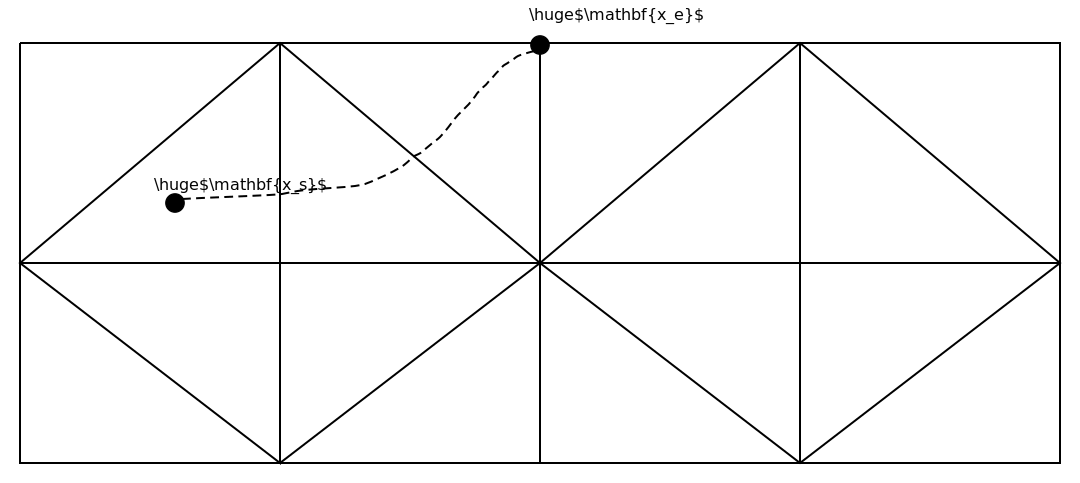
\includegraphics[width=\linewidth]{Figures/semi-lagrangian.pdf}
	\caption{Semi-Lagrangian Method}
	\label{fig:semi-lagrangian}
\end{figure}

Looking at \cref{fig:semi-lagrangian} we want to find the velocity (or any other quantity which is being advected) at time $t + \Delta t$ at point $\mathbf{x_e}$. In a Lagrangian framework this would be the same as the velocity of the (same) particle which at time $t$ was at $\mathbf{x_s}$ and has moved to $\mathbf{x_e}$ at time $t + \Delta t$. So our first problem is how to find $\mathbf{x_s}$. In order to do so we will linearize the velocity field go ``backwards'' in it. Let us elaborate, in a Lagrangian framework \cref{eq:general-three-way-split-advection} boils down to:

\begin{equation*}
	\frac{\partial\mathbf{x}}{\partial t} = \mathbf{u}
\end{equation*}
which we choose to approximate with a backward difference.

\begin{align*}
	\frac{\mathbf{x_e} - \mathbf{x_s}}{\Delta t} &= \mathbf{u}(\mathbf{x_e}, t) \\
	\mathbf{x_s} &= \mathbf{x_e} - \Delta t \mathbf{u}(\mathbf{x_e}, t)
\end{align*}

Now that we have found out the starting position of our imaginary particle, we are presented with another problem. We are not working in a Lagrangian framework and we are not simulating particles and it is almost certain that $\mathbf{x_s}$ will not be a vertex in our Eluerian mesh. The obvious solution is to interpolate the value inside the element using the values we have. Moreover it can be proven \cite{semi-lagrangian-stability} that the method is stable when we interpolate the value inside the element which surrounds it, the same cannot be stated if we decide to extrapolate and use values from elements which do not contain $\mathbf{x_s}$. In case $\mathbf{x_s}$ lies outside of the mesh we find the closest point on the boundary and take its value instead. Note that the position we found by this procedure is not the exact position of the particle which would end up in $\mathbf{x_e}$ beacuse we have used the velocity at $(\mathbf{x_e}, t)$ to approximate the velocity at $(\mathbf{x_e}, t + \Delta t)$, (see \cite{semi-lagrangian-stability} for an error estimate of this approach.)

The type of the mesh is of great importance when implementing the semi-Lagrangian algorithm. There are two properties of the mesh which we should consider. First is the shape of the element and the second is whether the mesh is structured. The term structured mesh is somewhat loose, by this we mean mesh whose elements have the same orientation and the same size, so that the indices of adjacent elements and nodes can be expressed via some explicit formula. An example of structured mesh with rectangular elements would be \cref{fig:structured-mesh}

\begin{figure}[H]
	\centering
	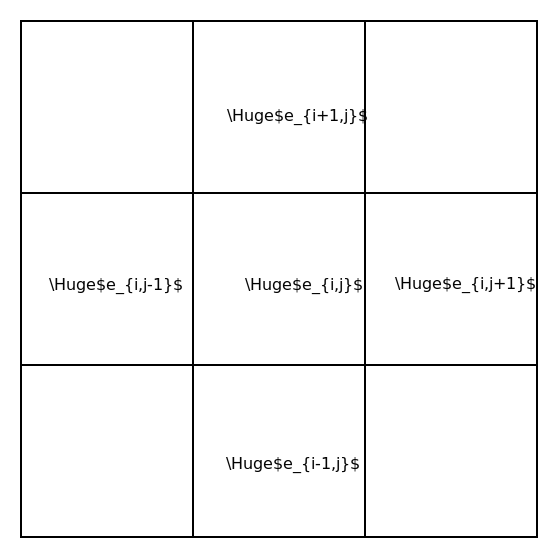
\includegraphics[width=0.4\linewidth]{Figures/structured-mesh.pdf}
	\caption{Structured mesh with rectangular elements.}\label{fig:structured-mesh}
\end{figure}

The advantage in working with such meshes (especially ones with rectangular elements) is that it is easy to find in which element a point lies. It all boils down to simple integer arithmetics. However when the mesh is unstructured we must iterate through all elements in order to find where a point lies. In our case we are working with unstructured triangular mesh. For this reason KD Tree data structure was implemented in order to accelerate the process of finding which element of the mesh contain a given point. It has complexity of $O(\log{n})$ for searching (assuming the tree is balanced) which element contains a point where $n$ is the total number of elements. Also it has another useful property: it can accelerate finding of the closest mesh point to another arbitrary point, although the worst case has complexity $O(n)$ it is rarely reached and on average it has complexity $O(\log{n})$. Assuming a KD Tree is implemented and filled with the elements of the mesh, a pseudo code for the advection phase is presented.

\begin{algorithm}[H]
\centering
\caption{Semi-Lagrangian Advection}\label{alg:Semi-Lagrangian-Advection}
\begin{algorithmic}[1]
		\Procedure{advect}{$KDTree, nodesIn, \Delta t$}
			\State $nodesOut \gets nodesIn$
			\ForAll{velocityNode $\in$ nodesIn}
				\State $\vecf{x_s} \gets velocityNode.position - velocityNode.velocity\Delta t $
				\If{$pointInMesh(KDTree, \vecf{x_s})$}
					\State $element \gets findElement(KDTree, \vecf{x_s})$
					\State $nodesOut.velocity \gets interpolate(\vecf{x_s}, element.velocityNodes)$
				\Else
					\State $closestVelocityNode \gets findClosestNode(KDTree, \vecf{x_s})$
					\State $nodesOut.velocity \gets closestVelocityNode.velocity$
				\EndIf
			\EndFor
		\EndProcedure
		\Return nodesOut
\end{algorithmic}
\end{algorithm}

\paragraph{Finite Element Method}
Now that we have a stable algorithm for the advection phase we can state the Finite Element Method for the given three way split using implicit Euler method for the diffusion.


\begin{align}
	&\mathbf{Q^A} = advect(KDTree, \mathbf{Q^{i}}, \Delta t) \label{eq:_adv-diff-split-advect}\\
		&\left(\begin{bmatrix}
		\mathbf{M} & 0 \\
		0 & \mathbf{M}
	\end{bmatrix} + \nu\Delta t\begin{bmatrix}
		\mathbf{K} & 0 \\
		0 & \mathbf{K}
	\end{bmatrix}\right)\begin{bmatrix}
		\vecf{Q^{B}_1} \\
		\vecf{Q^{B}_2}
	\end{bmatrix} = \begin{bmatrix}
		\mathbf{M} & 0 \\
		0 & \mathbf{M}
	\end{bmatrix}\begin{bmatrix}
		\vecf{Q^{A}_1} \\
		\vecf{Q^{A}_2}
	\end{bmatrix} \label{eq:_adv-diff-split-diffuse}\\
	&\mathbf{K_p}\vecf{P}^i = -\frac{1}{\Delta t} \begin{bmatrix}
		\mathbf{B_1} & \mathbf{B_2}
	\end{bmatrix} \begin{bmatrix}
		\vecf{Q^{B}_1} \\
		\vecf{Q^{B}_2}
	\end{bmatrix} \label{eq:_adv-diff-split-pressure}\\
	&\begin{bmatrix}
		\mathbf{M} & 0 \\
		0 & \mathbf{M}
	\end{bmatrix} \begin{bmatrix}
		\vecf{Q^{i+1}_1} \\
		\vecf{Q^{i+1}_2}
	\end{bmatrix} =	\begin{bmatrix}
		\mathbf{M} & 0 \\
		0 & \mathbf{M}
	\end{bmatrix} \begin{bmatrix}
		\vecf{Q^{B}_1} \\
		\vecf{Q^{B}_2}
	\end{bmatrix} - \Delta t \begin{bmatrix}
		\vecf{B_{p,1}} \\
		\vecf{B_{p,2}}
	\end{bmatrix} \vecf{P}^i \label{eq:_adv-diff-split-velicity-mass}
\end{align}
where \cref{eq:_adv-diff-split-advect} uses \cref{alg:Semi-Lagrangian-Advection}.

Again, the Dirichlet BC are imposed in the usual way.

\subsection{Choice of elements}

Now we shall present the elements used in this work. First of all, let us note that generating a FEM mesh is a large subject on its own and falls out of the scope of this work. Wolfram Mathematica was used to generate the FEM meshes used here. As of this date there is no built-in way to generate curved isoparametric elements with Wolfram Mathematica. For the direct approach we have used the $P_{-1}P_0$ non-conforming Crouzeix-Raviart element (see \cref{fig:P1P0-CR-Standard}). While it does not satisfy the LBB condition it can be proven \cite{Larson-Bengzon} that it is stable. It has the advantage of being divergence free and is computationally cheap. Using $P_{-1}P_0$ with the direct approach will produce a smaller matrix, compared to using any higher order element, thus the non-linear solver should perform better. For the two operator splitting methods $P_2P_1$ (see \cref{fig:P2P1-Standard}) Taylor-Hood element was used, it satisfies the LBB condition and according to \cite{gresho-fem} it is ``the simplest second order element'' and an ``early favorite''.

\begin{figure}[H]
  \centering
  \includegraphics[width=\textwidth]{Figures/01_introduction/cr_element.pdf}
  \caption{$P_{-1}P_0$ non-conforming Crouzeix-Raviart standard element. The 3 degrees of freedom for the velocity are marked with a solid color, the single degree of freedom for the pressure is marked with a circle.}\label{fig:P1P0-CR-Standard}
\end{figure}

\begin{figure}[H]
  \centering
  \includegraphics[width=\textwidth]{Figures/01_introduction/tylor_hood_element.pdf}
  \caption{$P_2P_1$ Taylor-Hood standard element. The 6 degrees of freedom for the velocity are marked with a solid color, the 3 degrees of freedom for the pressure are marked with a circle.}\label{fig:P2P1-Standard}
\end{figure}

\section{The CSR sparse matrix format}
We have chosen store the FEM matrices in the Compressed Sparse Row (CSR) format, which we shall describe briefly. For more information about other sparse matrix formats (see \cite{saad-sparse}). Let us denote the number of nonzero elements in a matrix with $nnz$ and the number of rows with $m$. The CSR format consists of 3 arrays, one real array \textit{NZ} of size $nnz$ containing the nonzero entries of the matrix, one integer array \text{Pos} of size $nnz$ containing the column for each nonzero entry and one integer array \text{Start} of size $m + 1$ containing the start index in \text{Pos} for each row of the matrix, the last element of the \text{Start} is usually an integer number equal to $nnz$. We note that the rows are sorted by their index in increasing fashion, but there is no such requirement of the columns and they can be stored in an arbitrary fashion, however for this work we choose to sort the columns in each row in increasing fashion, because this imporoves the cache locality in the computer implementation. Let us illustrate the format with an example, by applying it to the following matrix (see \cref{fig:example_sparse_matrix}).
\begin{figure}[H]
$$
\begin{bmatrix}
	1 & 0 & 0 & 2 & 0\\
	0 & 0 & 3 & 4 & 0\\
	0 & 0 & 5 & 0 & 6\\
	0 & 0 & 0 & 0 & 0\\
	7 & 0 & 8 & 9 & 0
\end{bmatrix}
$$
\caption{Example sparse matrix}\label{fig:example_sparse_matrix}
\end{figure}
The matrix stored in CSR format is shown in \cref{fig:example_csr_sparse_matrix}

\begin{figure}[H]
\centering
\begin{tabular}{l|ccccccccc}
\cline{2-10}
\textit{NZ}    & 1 & 2 & 3 & 4 & 5 & 6                      & 7 & 8 & \multicolumn{1}{c|}{9} \\ \cline{2-10}
\textit{Pos}   & 0 & 3 & 2 & 3 & 2 & 4                      & 0 & 2 & \multicolumn{1}{c|}{3} \\ \cline{2-10}
\textit{Start} & 0 & 2 & 4 & 6 & 6 & \multicolumn{1}{c|}{9} &   &   &                        \\ \cline{2-7}
\end{tabular}\caption{The matrix from \cref{fig:example_sparse_matrix} stored in CSR format. The indexing of the columns and the rows starts from 0.}\label{fig:example_csr_sparse_matrix}
\end{figure}

The memory needed to store a matrix in CSR format is $O(2*nnz + m)$. The space saved by compressing repeating row indexes turns out to be non-negligible \cite{saad-sparse}.

The number of nonzero elements in row $i$ can be found by $Start[i+1] - Start[i]$, the format allows for having empty rows, then $Start[i+1] - Start[i] = 0$. To find the next row with nonzero entries one shall iterate to find the first $i$ for which the $Start[i+1] - Start[i] \neq 0$.

This format is not flexible. Adding and removing nonzero entries after the sparse matrix is initialized would require shifting the \textit{NZ} and \textit{Pos} arrays with $O(nnz)$ time complexity and updating the values in the \textit{Start} array for $O(m)$, yielding total of $O(2*nnz) + O(m)$ operations which is considered to be slow. Despite the lack of flexibility this format allows for efficient implementation of matrix vector multiplication (see \cite{saad-sparse}).

\section{Solving Linear Systems of Equations}
Usually systems of equations which arise when applying numerical methods for differential equations have sparse matrices. This is true for the matrices in \crefrange{eq:_adv-diff-split-diffuse}{eq:_adv-diff-split-velicity-mass} and for the matrix in \cref{eq:2D_DFG_Direct_Crank-Nicholson}. In the course of this work various methods for solving linear systems with sparse matrices were studied. In this section we shall consider solving \crefrange{eq:_adv-diff-split-diffuse}{eq:_adv-diff-split-velicity-mass} which have symmetric positive definite matrices. Systems with such matrices are most commonly solved using the Conjugate Gradient method, which we shall discuss in this section. For information about sparse matrix formats and other methods for solving linear systems (which might be needed should \cref{eq:2D_DFG_Direct_Crank-Nicholson} be considered for solving the differential problem) refer to \cite{saad-sparse}.

\subsection{Conjugate Gradient}
The Conjugate Gradient method is one of the most famous and most studied methods for solving linear systems. It is part of the Krylov family of methods. The method is a special case of Incomplete Orthogonalization Method. In the case of SPD matrices it can be shown that each new direction can be represented with a short recurrency, thus only 3 vectors should be stored at a time. For full derivation and detailed explanation of the method refer to \cite{saad-sparse}. Here we shall present only pseudocode for the method.

\begin{algorithm}[H]
\centering
\caption{Conjugate Gradient Method solving $Ax=b$ with an initial guess $x_0$}\label{alg:CG}
\begin{algorithmic}[1]
		\Procedure{CG}{$A, b, x_0$}
			\State $r_0 \gets b - Ax_0$
			\State $p_0 \gets r_0$
			\For{$j \gets 0, 1, \dots$ until convergence}
				\State $\alpha_j \gets \frac{(r_j, r_j)}{(Ap_j, p_j)}$
				\State $x_{j+1} \gets x_j + \alpha_j p_j$
				\State $r_{j+1} \gets r_j - \alpha_j Ap_j$
				\State $\beta_j \gets \frac{(r_{j+1}, r_{j+1})}{(r_j, r_j)}$
				\State $p_{j+1} \gets r_{j+1} + \beta_j p_j$
			\EndFor
			\State \Return $x_{j+1}$
		\EndProcedure
\end{algorithmic}
\end{algorithm}

\subsection{Zero Fill-in Incomplete Cholesky Preconditioner (IC0)}
The point of preconditioning is to improve the condition number of the matrix. Using a good preconditioner can significantly lower the number of iterations needed by the method to converge. A good preconditioner for the CG method should not change the properties of the matrix and keep it SPD. Let us assume that such a preconditioner is used. Multiplying two sparse matrices often produces a dense matrix, thus it is not wise to precondition the system by directly multiplying the matrix. A better approach incorporates the preconditioner in each iteration. There are few ways to do so in the CG with a preconditioner which is also SPD. The following algorithm is one of those proposed in \cite{saad-sparse}.

\begin{algorithm}[H]
\centering
\caption{Preconditioned Conjugate Gradient Method solving $Ax=b$ with an initial guess $x_0$}\label{alg:pcg}
\begin{algorithmic}[1]
		\Procedure{PCG}{$A, M^{-1} b, x_0$}
			\State $r_0 \gets b - Ax_0$
			\State $z_0 \gets M^{-1}r_0$\label{alg-line:apply-preconditioner}
			\State $p_0 \gets z_0$
			\For{$j \gets 0, 1, \dots$ until convergence}
				\State $\alpha_j \gets \frac{(r_j, z_j)}{(Ap_j, p_j)}$
				\State $x_{j+1} \gets x_j + \alpha_j p_j$
				\State $r_{j+1} \gets r_j - \alpha_j Ap_j$
				\State $z_{j+1} \gets M^{-1}r_{j+1}$
				\State $\beta_j \gets \frac{(r_{j+1}, z_{j+1})}{(r_j, z_j)}$
				\State $p_{j+1} \gets z_{j+1} + \beta_j p_j$
			\EndFor
			\State \Return $x_{j+1}$
		\EndProcedure
\end{algorithmic}
\end{algorithm}

Given \cref{alg:pcg} a logical choice for a preconditioner is the Cholesky decomposition of the matrix $A = LL^T$. However we are not guaranteed that $L$ will be sparse even when $A$ is. Thus we want to find $\widetilde{L}$ which is close to $L$ and $\widetilde{L}\widetilde{L}^T$ which is close to $A$. We choose $\widetilde{L}$ such that it has the same nonzero pattern as the lower triangular part of $A$. This preconditioner can be computed via the standard Cholesky decomposition procedure by dropping elements $l_{i,j}$ for i and j such that $a_{i,j} = 0$. Now when the preconditioner and the matrix share the same non-zero pattern the preconditioner could be represented only by its values. We choose to store $\widetilde{L}^T$ in order to make the memory access more regular and improve the performance.

\section{Numerical Experiment}
Let us now show the plot of the solution of \cref{eq:laminar_differential_form}, afther the 100 iterations with step $\Delta t = 0.01$, produced by solving \cref{eq:2D_DFG_Direct_Crank-Nicholson} and compare it to the solution of the same differential problem, but solved by solving \cref{eq:chorin_split_fem} with $\Delta t = 0.01$ and\crefrange{eq:_adv-diff-split-advect}{eq:_adv-diff-split-velicity-mass} with $\Delta t = 0.01$.\footnote{There is a stylistic difference between \cref{fig:p0p1-plot}, \cref{fig:chorin-plot} and \cref{fig:advection-diffusion-plot}. This is because the solutions for the direct approach and the Chorin split were obtained by a prototype written in Wolfram Mathematica while the last plot was produced by the final version of the code written in C++ and CUDA.} We can observe that \cref{eq:chorin_split_fem}  and \crefrange{eq:_adv-diff-split-advect}{eq:_adv-diff-split-velicity-mass} produce similar results, while solving \cref{eq:2D_DFG_Direct_Crank-Nicholson} with $P_{-1}P_0$ element produces worse results, especially near the boundaries. It must be noted, however, that this comparison is not completely honest, because the two splitting methods use higher order elements. A solution of \cref{eq:laminar_differential_form} with the LBB unstable $P_1P_1$ element could be found in \cite{Larson-Bengzon}. It is also better than the result achieved by \cref{eq:2D_DFG_Direct_Crank-Nicholson}. This leads us to believe that an element of at least first degree polynomial space should be used for the pressure. The compuational cost of solving nonlinear systems and the bad results produced with $P_{-1}P_0$ element have discouraged us from further investigation of \cref{eq:2D_DFG_Direct_Crank-Nicholson}.

\begin{figure}[H]
\centering
\includegraphics[width=\textwidth]{Figures/01_introduction/P1P0_100.pdf}
\caption{Solution for laminar flow via \cref{eq:2D_DFG_Direct_Crank-Nicholson} after 100 iterations with $\Delta t = 0.01$ }\label{fig:p0p1-plot}
\end{figure}

\begin{figure}[H]
\centering
\includegraphics[width=\textwidth]{Figures/01_introduction/P2P1_100.pdf}
\caption{Solution for laminar flow via \cref{eq:chorin_split_fem} after 100 iterations with $\Delta t = 0.01$ }\label{fig:chorin-plot}
\end{figure}

\begin{figure}[H]
\centering
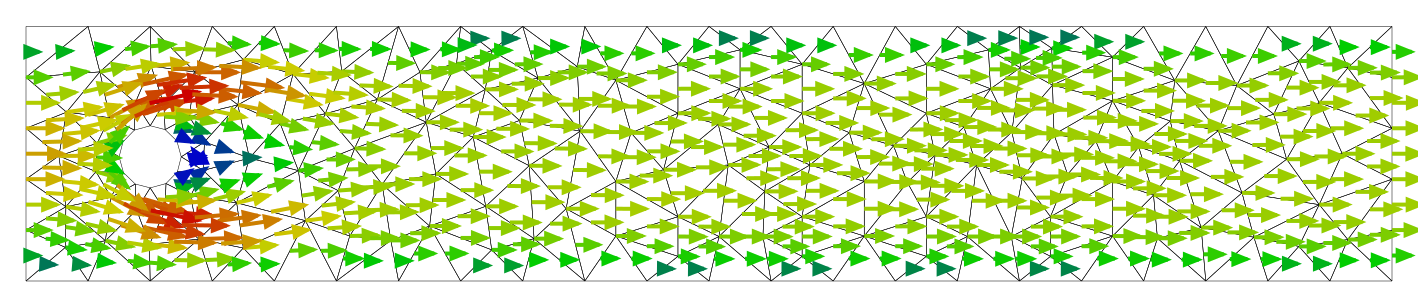
\includegraphics[width=\textwidth]{Figures/01_introduction/P2P1_adv_diff_100.pdf}
\caption{Solution for laminar flow via \crefrange{eq:adv-diff-split-advect}{eq:adv-diff-split-diffuse} after 100 iterations with $\Delta t = 0.01$.}\label{fig:advection-diffusion-plot}
\end{figure}

\section{Conclusion}
We have decided to further develop the three way splitting method. This is based on a few properties. First, the numerical experiment did not show any problems with the accuracy for the given task. Second, the semi-Lagrangian advection method is perfect for multithreaded CPU and GPU implementation. Third, the method can be used with an arbitrary step size and the step size is not tied to the spatial step (element size).
\chapter{Parallel implementation}\label{ch:implementation-details}
In this chapter we shall present techniques used to improve the performance of the simulation. We shall present both CPU and GPU parallelization techniques and compare them. The performance will be measured on two machines Computer 1: CPU - Intel(R) Core(TM) i7-3632QM CPU @ 2.20GHz (4 cores, 8 threads), 2 blocks of 4GB SODIMM DDR3 Synchronous 800 MHz RAM and Computer 2: CPU - Intel(R) Core(TM) i7-9700 CPU @ 3.00GHz (8 cores, 8 threads) and 4 blocks of 16GB DDR4 1333 MHz RAM, GPU 1 - NVidia A5000. We shall measure two scenarios - laminar and turbulent flow. Both scenarios will be tested with the following mesh on both machines.

\begin{table}[H]
\centering
\begin{tabular}{|c|r|r|}
\hline
\multicolumn{1}{|l|}{} & \multicolumn{1}{c|}{Mesh} \\ \hline
Elements               & 305854                      \\ \hline
Velocity Nodes         & 613458                      \\ \hline
Pressure Nodes         & 153802                      \\ \hline
\end{tabular}
\end{table}

Let us first sum up the problem and the algorithm used to solve it. We are looking for an approximate solution to the Navier-Stokes equations for a laminar (\cref{eq:laminar_differential_form_recap}) and a turbulent(\cref{eq:turbulent_differential_form_recap}) flow.
\begin{equation}\label{eq:laminar_differential_form_recap}
\begin{aligned}
  &\frac{\partial\mathbf{u}}{\partial t} + \mathbf{u} \cdot \nabla\mathbf{u} = -\nabla p + \nu\Delta\mathbf{u}, &&\left(\mathbf{x}, t\right) \in \Omega \times J \\
  &\nabla \cdot \mathbf{u} = 0, &&\left(\mathbf{x}, t\right) \in \Omega \times J \\
  &\mathbf{u} = 0, &&\left(\mathbf{x}, t\right) \in \left(\Gamma_1 \cup \Gamma_3 \cup \Gamma_5\right) \times J \\
  &\mathbf{u} = \left(\frac{1.2y\left(0.41 - y\right)}{0.41^2}, 0\right), &&\left(\mathbf{x}, t\right) \in \Gamma_4 \times J \\
  &\nu\frac{\partial\mathbf{u}}{\partial\mathbf{n}} - p\mathbf{n} = 0, &&\left(\mathbf{x}, t\right) \in \Gamma_2 \times J \\
\end{aligned}
\end{equation}

\begin{equation}\label{eq:turbulent_differential_form_recap}
\begin{aligned}
  &\frac{\partial\mathbf{u}}{\partial t} + \mathbf{u} \cdot \nabla\mathbf{u} = -\nabla p + \nu\Delta\mathbf{u}, &&\left(\mathbf{x}, t\right) \in \Omega \times J \\
  &\nabla \cdot \mathbf{u} = 0, &&\left(\mathbf{x}, t\right) \in \Omega \times J \\
  &\mathbf{u} = 0, &&\left(\mathbf{x}, t\right) \in \left(\Gamma_1 \cup \Gamma_3 \cup \Gamma_5\right) \times J \\
  &\mathbf{u} = \left(\frac{6y(0.41-y)}{0.41^2}, 0\right), &&\left(\mathbf{x}, t\right) \in \Gamma_4 \times J \\
  &\nu\frac{\partial\mathbf{u}}{\partial\mathbf{n}} - p\mathbf{n} = 0, &&\left(\mathbf{x}, t\right) \in \Gamma_2 \times J \\
\end{aligned}
\end{equation}

To do so at each time step we apply \crefrange{eq:adv-diff-split-advect}{eq:adv-diff-split-velicity-mass}:

\begin{align}
	&\mathbf{Q^A} = advect(KDTree, \mathbf{Q^{i}}, \Delta t) \label{eq:adv-diff-split-advect}\\
		&\left(\begin{bmatrix}
		\mathbf{M} & 0 \\
		0 & \mathbf{M}
	\end{bmatrix} + \nu\Delta t\begin{bmatrix}
		\mathbf{K} & 0 \\
		0 & \mathbf{K}
	\end{bmatrix}\right)\begin{bmatrix}
		\vecf{Q^{B}_1} \\
		\vecf{Q^{B}_2}
	\end{bmatrix} = \begin{bmatrix}
		\mathbf{M} & 0 \\
		0 & \mathbf{M}
	\end{bmatrix}\begin{bmatrix}
		\vecf{Q^{A}_1} \\
		\vecf{Q^{A}_2}
	\end{bmatrix} \label{eq:adv-diff-split-diffuse}\\
	&\mathbf{K_p}\vecf{P}^i = -\frac{1}{\Delta t} \begin{bmatrix}
		\mathbf{B_1} & \mathbf{B_2}
	\end{bmatrix} \begin{bmatrix}
		\vecf{Q^{B}_1} \\
		\vecf{Q^{B}_2}
	\end{bmatrix} \label{eq:adv-diff-split-pressure}\\
	&\begin{bmatrix}
		\mathbf{M} & 0 \\
		0 & \mathbf{M}
	\end{bmatrix} \begin{bmatrix}
		\vecf{Q^{i+1}_1} \\
		\vecf{Q^{i+1}_2}
	\end{bmatrix} =	\begin{bmatrix}
		\mathbf{M} & 0 \\
		0 & \mathbf{M}
	\end{bmatrix} \begin{bmatrix}
		\vecf{Q^{B}_1} \\
		\vecf{Q^{B}_2}
	\end{bmatrix} - \Delta t \begin{bmatrix}
		\vecf{B_{p,1}} \\
		\vecf{B_{p,2}}
	\end{bmatrix} \vecf{P}^i \label{eq:adv-diff-split-velicity-mass}
\end{align}
where the method $advect$ is \cref{alg:Semi-Lagrangian-Advection}.

\section{CPU multithreading}
Our end goal is to implement all algorithms on a GPU. However we need a baseline multithreaded CPU algorithm so that we can measure the pros and cons of using GPU for simulations. In this section we shall present the steps which were taken in order to multithread the chosen method on CPU.

We shall measure the time it takes for the algorithm to compute 1s of simulation time with time step 0.01 i.e. 100 time steps. The baseline for the measurements is the single threaded algorithm. \crefrange{tab:computer1-laminar-baseline}{tab:computer2-turbulent-baseline} present the time spent in each step of the algorithm (\cref{eq:adv-diff-split-advect} - Step 1, \cref{eq:adv-diff-split-diffuse} - Step 2, \cref{eq:adv-diff-split-pressure} - Step 3 and \cref{eq:adv-diff-split-velicity-mass} - Step 4 and the assembling of the corresponding matrices). The measurement is done using C++ timers (std::chrono::steady\_clock) placed at the beginning and ending of each function. The data for executing the algorithm is gathered over 11 sequential runs of the algorithm on Computer 1 and Computer 2 for the given mesh.
\begin{table}[H]
\centering
\begin{tabular}{|c|c|c|c|c|c|c|c|}
\hline
\multirow{3}{*}{} & \multicolumn{7}{c|}{Computer 1}                                                                                                                                       
\\ \cline{2-8}
& Step 1 & Step 2 & Step 3 & Step 4 & \begin{tabular}[c]{@{}c@{}}CG \\ (Total)\end{tabular} & \begin{tabular}[c]{@{}c@{}}Matrix\\ Assembling\end{tabular} & \begin{tabular}[c]{@{}c@{}}Total \\ Time\end{tabular} \\ \hline
\begin{tabular}[c]{{@{{}}c@{{}}}}Mean \\ Time\end{tabular}  & 79.75s & 138.33s & 505.50s & 44.47s & 688.30s & 20.80s & 794.82s\\ \hline SD & 0.64s&3.83s&3.62s&1.30s&8.76s&0.38s&10.01s\\ \hline Median & 80.20s&141.05s&508.06s&45.39s&694.50s&21.07s&801.89s\\ \hline Min & 79.30s&135.62s&502.94s&43.55s&682.11s&20.54s&787.74s\\ \hline Max & 80.20s&141.05s&508.06s&45.39s&694.50s&21.07s&801.89s\\ \hline
\end{tabular}
\caption{Execution time on 1 thread of Computer 1 for solving for laminar flow via \crefrange{eq:adv-diff-split-advect}{eq:adv-diff-split-velicity-mass} over the given mesh with $\Delta t = 0.01$ and Conjugate Gradient method used for solving the linear system.}\label{tab:computer1-laminar-baseline}
\end{table}

\begin{table}[H]
\centering
\begin{tabular}{|c|c|c|c|c|c|c|c|}
\hline
\multirow{3}{*}{} & \multicolumn{7}{c|}{Computer 2}                                                                                                                                       
\\ \cline{2-8}
& Step 1 & Step 2 & Step 3 & Step 4 & \begin{tabular}[c]{@{}c@{}}CG \\ (Total)\end{tabular} & \begin{tabular}[c]{@{}c@{}}Matrix\\ Assembling\end{tabular} & \begin{tabular}[c]{@{}c@{}}Total \\ Time\end{tabular} \\ \hline
\begin{tabular}[c]{{@{{}}c@{{}}}}Mean \\ Time\end{tabular}  & 60.32s & 101.12s & 398.50s & 30.31s & 529.93s & 11.82s & 605.48s\\ \hline SD & 0.15s&0.57s&1.85s&0.05s&2.14s&0.04s&2.27s\\ \hline Median & 60.31s&100.96s&398.29s&30.33s&529.86s&11.84s&605.45s\\ \hline Min & 60.03s&100.56s&395.98s&30.19s&526.75s&11.76s&602.09s\\ \hline Max & 60.54s&102.54s&402.81s&30.37s&534.01s&11.87s&609.62s\\ \hline
\end{tabular}
\caption{Execution time on 1 thread of Computer 2 for solving for laminar flow via \crefrange{eq:adv-diff-split-advect}{eq:adv-diff-split-velicity-mass} over the given mesh with $\Delta t = 0.01$ and Conjugate Gradient method used for solving the linear system.}\label{tab:computer2-laminar-baseline}
\end{table}


%%%%%%%%%%%%%%%%%%%%%%%%%%%%%%%%%%%%%%%%%%%%%%%%%%%%%%%%%%%%%%%%%%%%%%%%%%
%%%%%%%%%%%%%%%%%%%%%%%%%%% TURBULENT %%%%%%%%%%%%%%%%%%%%%%%%%%%%%%%%%%%%
%%%%%%%%%%%%%%%%%%%%%%%%%%%%%%%%%%%%%%%%%%%%%%%%%%%%%%%%%%%%%%%%%%%%%%%%%%
\begin{table}[H]
\centering
\begin{tabular}{|c|c|c|c|c|c|c|c|}
\hline
\multirow{3}{*}{} & \multicolumn{7}{c|}{Computer 1}                                                                                                                                       
\\ \cline{2-8}
& Step 1 & Step 2 & Step 3 & Step 4 & \begin{tabular}[c]{@{}c@{}}CG \\ (Total)\end{tabular} & \begin{tabular}[c]{@{}c@{}}Matrix\\ Assembling\end{tabular} & \begin{tabular}[c]{@{}c@{}}Total \\ Time\end{tabular} \\ \hline
\begin{tabular}[c]{{@{{}}c@{{}}}}Mean \\ Time\end{tabular}  & 80.35s & 196.81s & 597.43s & 55.31s & 849.54s & 20.45s & 956.29s\\ \hline SD & 0.83s&5.57s&3.18s&0.77s&9.52s&0.08s&10.45s\\ \hline Median & 80.94s&200.74s&599.68s&55.86s&856.28s&20.51s&963.68s\\ \hline Min & 79.76s&192.87s&595.18s&54.76s&842.81s&20.40s&948.90s\\ \hline Max & 80.94s&200.74s&599.68s&55.86s&856.28s&20.51s&963.68s\\ \hline
\end{tabular}
\caption{Execution time on 1 thread of Computer 1 for solving for turbulent flow via \crefrange{eq:adv-diff-split-advect}{eq:adv-diff-split-velicity-mass} over the given mesh with $\Delta t = 0.01$ and Conjugate Gradient method used for solving the linear system.}\label{tab:computer1-turbulent-baseline}
\end{table}

\begin{table}[H]
\centering
\begin{tabular}{|c|c|c|c|c|c|c|c|}
\hline
\multirow{3}{*}{} & \multicolumn{7}{c|}{Computer 2}                                                                                                                                       
\\ \cline{2-8}
& Step 1 & Step 2 & Step 3 & Step 4 & \begin{tabular}[c]{@{}c@{}}CG \\ (Total)\end{tabular} & \begin{tabular}[c]{@{}c@{}}Matrix\\ Assembling\end{tabular} & \begin{tabular}[c]{@{}c@{}}Total \\ Time\end{tabular} \\ \hline
\begin{tabular}[c]{{@{{}}c@{{}}}}Mean \\ Time\end{tabular}  & 61.22s & 143.49s & 541.06s & 37.69s & 722.23s & 11.90s & 798.78s\\ \hline SD & 0.31s&0.77s&3.23s&0.17s&3.97s&0.12s&4.25s\\ \hline Median & 61.35s&143.62s&542.91s&37.73s&724.74s&11.89s&801.48s\\ \hline Min & 60.74s&142.42s&535.43s&37.39s&716.07s&11.75s&792.43s\\ \hline Max & 61.71s&144.89s&544.70s&38.03s&727.36s&12.17s&804.32s\\ \hline
\end{tabular}
\caption{Execution time on 1 thread of Computer 2 for solving for turbulent flow via \crefrange{eq:adv-diff-split-advect}{eq:adv-diff-split-velicity-mass} over the given mesh with $\Delta t = 0.01$ and Conjugate Gradient method used for solving the linear system.}\label{tab:computer2-turbulent-baseline}
\end{table}

Although these two examples are not comprehensive and more tests with different scenarios must be made, they give us a few hints about the behaviour of the program. The bulk of the time is spent in the Conjugate Gradient method, with \cref{eq:adv-diff-split-pressure} being the most computationally expensive. The matrix used when solving the Pressure Poisson equation is smaller than the other matrices, thus it is logical to assume that the method needs more iterations in order to converge. It looks like turbulent flows need more iterations of the Conjugate Gradient method, most likely because the flow is less ``predictable''.

\subsection{Building the FEM matrices}
The case we are studying is restricted to geometry which is not changing with time. In this case the matrices used by the FEM are constant and are built once at the beginning of the solution. The problem with assembling FEM matrices in a multithreaded fashion is similar to computing IC0 preconditioners in multithreaded fashion. It depends on the topology of the mesh. Usually graph coloring algorithms are used in order to find which elements will not interfere with one another and fill in the matrix for them in parallel. This technique is also not trivial. Given the fact that the matrices are assembled once and that the assembling takes a small fraction of time, a simpler technique was used - each matrix was computed on a separate thread. Since there are 5 matrices we need 5 threads. This way the assembling of the matrices takes time equal to the time for the most expensive matrix (given that we have 5 or more threads at our disposal). This is a simplistic technique but it gives satisfactory results. Implementing graph coloring is left for further research.

\subsection{Multithreading the advection phase}\label{sec:mt-advection}
\subsubsection{A brief introduction to the KD Tree data structure}
KD Trees are binary trees which are very commonly used in ray tracing for acceleration of ray-mesh intersections \cite{pbrt} and in artificial intelligence for solving the k nearest neighbours (KNN) problem \cite{knn-ai}. Originally they were used to handle large sets of points in a k dimensional space (thus the name KD Tree), but they are trivially extendable to handle different kinds of geometrical objects e.g. k dimensional spheres, triangles in 2D and 3D. We will focus on building KD Tree for the 2D space, which will be used to accelerate two types of queries: find in which triangle of a FEM mesh a given point lies and find the nearest node of our FEM mesh to a given point in space.

We begin with a procedure for building a KD Tree (see \cref{alg:build-kd}). Each non-leaf node is a tuple of the form (Axis, Splitting Point, Left Child, Right Child), leaf nodes contain a list of elements assigned to them during the construction of the tree. Initially we begin with a root node, an axis aligned bounding box for the FEM mesh and a set of triangles representing the FEM mesh. The axis aligned bounding boxes are represented with their lower left and upper right vertices. At each point we choose an axis and a point along the axis. Then we imagine that there is a line orthogonal to the axis and containing the selected point. All elements on one side of the line are assigned to one of the children. The other elements (which are on the other side of the line) are assigned to the other (see \cref{fig:kd-build}). Should a triangle lie in both subspaces defined by the line it is assigned to both children. This continues recursively until the count of the triangles in a node gets below some cutoff value or the maximal allowed depth is reached.

\begin{figure}
  \centering
  \includegraphics[width=0.5\textwidth]{Figures/kd-example.pdf}
  \caption{The chosen axis is the $y$ axis and the splitting point is 6. A line passing through (0, 6) and orthogonal to the $y$ axis separates the space into two subspaces. Triangles 1 and 2 will be in the right subtree, triangles 2, 3, 4 will be in the left subtree.}\label{fig:kd-build}
\end{figure}

\begin{algorithm}[H]
\centering
\caption{Build KD Tree}\label{alg:build-kd}
\begin{algorithmic}[1]
		\Procedure{BuildKD}{$node, triangles, AABB, depth$}
			\If{$count(triangles) \leq leafSize \lor depth \geq maxDepth$}
				\State \Return makeLeaf(triangles)
			\EndIf
			\State $axis \gets chooseAxis()$
			\State $split \gets chooseSplitPoint()$
			\State $node.axis \gets axis$
			\State $node.split \gets split$
			\State $splitBox(AABB, axis, split, leftAABB, rightAABB)$
			\State $leftTriangles \gets \{\}$
			\State $rightTriangles \gets \{\}$
			\ForAll{t $\in$ triangles}
				\If{$t.A[axis] \leq split \lor t.B[axis] \leq split \lor t.C[axis] \leq split$}
					\State insert(leftTriangles, t)
				\EndIf
				\If{$t.A[axis] \geq split \lor t.B[axis] \geq split \lor t.C[axis] \geq split$}
					\State insert(rightTriangles, t)
				\EndIf
			\EndFor
			\State $root.left \gets BuildKD(leftTriangles, leftAABB, depth + 1)$
			\State $root.right \gets BuildKD(rightTriangles, rightAABB, depth + 1)$
			\State \Return root
		\EndProcedure
\end{algorithmic}
\end{algorithm}

Next we present a procedure (see \cref{alg:get-triangle}) which finds which triangle (if any) contains a point. It is a straightforward task, we just need to traverse the tree. If the given point lies in the left bounding box we follow the left child, otherwise, we follow the right. When we reach a leaf, we need to iterate all triangles in it to see if the point lies in any of them. It is obvious that, given a balanced tree, the complexity of this task is $O(\log{m})$ where m is the number of triangles in the tree.

\begin{algorithm}[H]
\centering
\caption{Find in which triangle a point lies}\label{alg:get-triangle}
\begin{algorithmic}[1]
	\Procedure{FindTriangle}{$node, point$}
		\If{isLeaf(node)}
			\ForAll{$triangle \in node.triangles$}
				\If{$point \in triangle$}
					\State \Return triangle
				\EndIf
			\EndFor
			\Return null
		\EndIf
		\If{$point[node.axis] \leq node.split$}
			\State \Return FindTriangle(node.left, point)
		\Else
			\State \Return FindTriangle(node.right, point)
		\EndIf
	\EndProcedure
\end{algorithmic}
\end{algorithm}

Finding the nearest neighbour is a bit more complex than checking in which triangle a point lies, but the idea is basically the same. The problem is that the nearest mesh point could lie on the opposing side of the splitting axis and thus it is not enough to traverse the tree until reaching the first leaf (see \cref{fig:nearest-neighbour}). To find the nearest point we start traversing the tree recursively, but we need to visit both children of a given node. There is a common optimization which significantly improves the performance for the average case. Let us call the child whose subspace contains the point from the query the near child and the other child the far child. When traversing the tree we must always go to the near child and traverse down to the far child only when distance to the separating plane is less than the distance between the query point and the current nearest neighbour, \cref{alg:nearest-neighbour} presents this idea. Let us note that, although this improves the average case complexity to $O(\log{n})$ where n is the number of points, the worst case, however, is still $O(n)$.

\begin{figure}[H]
  \centering
  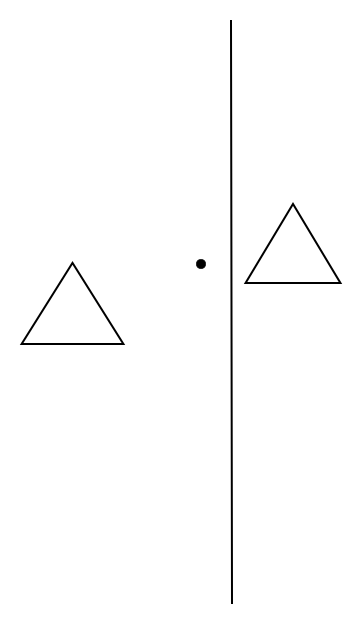
\includegraphics[scale=0.4]{Figures/nearest-neighbour.pdf}
  \caption{The nearest point of the mesh does not always lie in the same subspace, with respect to the separating axis, as the input point.}
  \label{fig:nearest-neighbour}
\end{figure}

\begin{algorithm}[H]
\centering
\caption{Find the nearest point from a FEM mesh to a given point in space}\label{alg:nearest-neighbour}
\begin{algorithmic}[1]
	\Procedure{NearestNeighbour}{$node, point, currentResult$}
		\If{isLeaf(node)}
			\State $result \gets currentResult$
			\ForAll{$triangle \in node.triangles$}
				\ForAll{$node \in triangle$}
					\If{$distance(node, point) < result.distance$}
						\State $result.distance \gets distance(node, point)$
						\State $result.point \gets node$
					\EndIf
				\EndFor
			\EndFor
			\State \Return result
		\EndIf
		\State$near \gets node.left$
		\State$far  \gets node.right$
		\If{$point[node.axis] > node.split$}
			\State swap(near, far)
		\EndIf
		\State $result \gets NearestNeighbour(near, point, currentResult)$
		\If{$result.distance > abs(point[node.axis] - node.split)$}
			\State $result \gets NearestNeighbour(far, point, result)$
		\EndIf
		\State \Return result
	\EndProcedure
\end{algorithmic}
\end{algorithm}

\subsubsection{KD Tree implementation details}
Before discussing the multithreading part we shall give some implementation details about the KD Tree and a commentary on how it should be improved. The tree is built in a recursive top-down fashion. It is stored in a linear array, the root is stored at index 0. If a node has index $i$ in the array its left child is always stored at index $i+1$, while its right child is stored at some other index which is not important. In our case for a given node we first build its left subtree and then the right subtree. Thus the index of the right child is the first free index after the last node of the left subtree. Such ordering is cache friendly, because when we reach a node its left child will always be on the same cache line. The maximum allowed depth is 29 and in case a node has less than 16 triangles in it, it is made a leaf. The cutoff value of 16 does not have any specific reasoning behind it, different values were tested and there were no significant changes in runtime. The most important part of building a KD tree for this case is to make it as balanced as possible. At each step a splitting point along the splitting axis must be chosen such that the difference between the number of triangles on both of its sides is as small as possible. There are two -- questions how to choose the axis and how to choose the point. We select the axes in a round-robin fashion. Our strategy for choosing a split point is to split the bounding box of the parent node in the center, along the splitting axis, subdividing it into equal sized bounding boxes for each child. This strategy is rather simplistic and does not work well. For small meshes such as the given mesh it is tolerable and the run time is still dominated by the CG method, however should the given mesh become, say, 2 times larger  the runtime increases unproportionally, making the method borderline unusable. A better approach should be implemented. The simplest approach is to use the Quickselect algorithm \cite{introduction-to-algorithms} in order to find the median of the points in the current tree and use it as a splitting point when subdividing into subtrees. The algorithm has best and average case complexity of $O(n)$ where $n$ is the number of points, but worst case of $O(n^2)$. It was implemented and it significantly improved the tree traversal performance. However this increased the time needed to build the tree by a substantial amount. This happens because the algorithm must be executed for each node. Thus making it a viable choice when the simulation has a large amount of steps. Another option is to use the PICK algorithm \cite{pick}, it is a well known algorithm for finding the median of an array in deterministic $O(n)$ time. We have not tried to implement it. On one hand it is not trivial to implement on the other hand, although, it has asymptotically linear time, the constant (which is implied by the notation) is known to be large, thus making it slower than Quickselect with random pivot selection, until the data set becomes large enough. Due to this reason we think that it falls out of the scope of the current work. It would be interesting to implement it, however. Another approach worth trying is described in \cite{Balanced-KD-Tree}.

\subsubsection{Splitting the work between threads}
As it was already mentioned the semi-Lagrangian algorithm is trivial to parallelize. We shall use simple fork-join technique to do so. It is obvious that each quantity at each vertex (in our case only the velocity is advected, but  in general there can be other quantities such as temperature, concentration, etc.) can be advected on its own without interacting with the other advected quantities and other mesh vertices. Thus we shall split all velocity nodes into groups and each group should be scheduled to a separate CPU thread. For the implementation we use the Thread Building Blocks (TBB) multithreading library provided by Intel. It does the job of spawning threads and distributing work between them, while we shall only pass the function which will be executed on each thread. Next we present how this scales with multiple threads see( \crefrange{fig:advection_speedup_graph_laminar}{fig:advection_speedup_graph_turbulent}). For more detailed view refer to \cref{ch:stastical-data}

\subsubsection{Speedup results}
\begin{figure}[H]
  \centering
  \begin{subfigure}[b]{0.49\textwidth}
      \centering
      \includegraphics[width=\textwidth]{Figures/LaminarAdvectionSpeedUpC1.pdf}
      \caption{Computer 1}
  \end{subfigure}
  \begin{subfigure}[b]{0.49\textwidth}
      \centering
      \includegraphics[width=\textwidth]{Figures/LaminarAdvectionSpeedUpC2.pdf}
      \caption{Computer 2}
  \end{subfigure}
\caption{Scaling of \cref{eq:adv-diff-split-advect} solved via semi-Lagrangian method with $\Delta t = 0.01$ over the given mesh for laminar flow. Vertical bars represent 2 times the standard deviation of the measured speedup.}\label{fig:advection_speedup_graph_laminar}
\end{figure}

\begin{figure}[H]
  \centering
  \begin{subfigure}[b]{0.49\textwidth}
      \centering
      \includegraphics[width=\textwidth]{Figures/TurbulentAdvectionSpeedUpC1.pdf}
      \caption{Computer 1}
  \end{subfigure}
  \begin{subfigure}[b]{0.49\textwidth}
      \centering
      \includegraphics[width=\textwidth]{Figures/TurbulentAdvectionSpeedUpC2.pdf}
      \caption{Computer 2}
  \end{subfigure}
\caption{Scaling of \cref{eq:adv-diff-split-advect} solved via semi-Lagrangian method with $\Delta t = 0.01$ over the given mesh for turbulent flow. Vertical bars represent 2 times the standard deviation of the measured speedup.}\label{fig:advection_speedup_graph_turbulent}
\end{figure}

From the provided data we can see that the algorithm scales with increasing the number of threads. The standard deviation is low, meaning that the runtime does not fluctuate. One thing which should be noted is that according to the data, the achieved speedup for Computer 1 drops a bit when the mark of 5 threads is reached. After that the speedup still increases when the number of threads increases, but it is further from the expected one. This phenomenon is due to Intel Hyper-Threading technology. Computer 1 is a quad core computer. This means that in theory only 4 tasks can be executed in parallel, thus the speedup is much better in the range [2;4] threads. However modern CPUs have very complicated architecture. One CPU core contains multiple arithmetic units, pipelines, cache and branch predictors, etc. It often happens that one thread cannot fully utilize the CPU. Imagine the simplest case possible, the thread does only integer operations. In this case all floating point arithmetic units are idle. Intel Hyper-Threading technology addresses this issue, by presenting each physical core as 2 logical cores. This way through clever task scheduling the CPU can be utilized better. This technique has its limitations and it is obvious that using threads more than the number of cores does not mean that the performance should double. On the other hand Computer 2 has 8 core processor and does not support Hyper-Threading. We can see that the algorithm, indeed, continues scaling in an almost linear fashion even beyond the 4 threads mark.

\subsection{Conjugate Gradient}
Contrary to the advection, Conjugate Gradient cannot be multithreaded as a whole. However we can multithread each step of it: the matrix vector product, the vector additions and the dot product. All of these are trivially parallelizable on their own. TBB was used for this part as well. For the vector matrix product the matrix is split into blocks, each block containing some set of rows. Thus each CPU thread gets to compute all dot products of the rows in its block of the matrix and the vector which multiplies the matrix. For the vector additions we use a similar technique, the vectors are split in blocks and each CPU thread gets to add the parts of the two vectors in its block. For the dot product the built-in tbb::parallel\_deterministic\_reduce operation is used, it also uses the same idea, and splits the vectors into blocks, then each CPU thread computes the dot product of the subvectors in its block, this leaves us with an array $a_1, a_2, ... a_n$ of the computed (sub) dot products, which must be added together in order to compute the final result. What tbb::parallel\_deterministic\_reduce does is to provide specific order to all additions so that the result of the dot product is always deterministic. The downside of it is that TBB cannot dynamically split the workload and the sizes of each block must be defined by the programmer. We have empirically chosen blocks of size 8192. As we mentioned the Conjugate Gradient cannot be multithreaded as a whole, and the reason is the dot product which acts as a barrier between the separate phases of the algorithm. Next in \cref{fig:laminar-scaling} and \cref{fig:turbulent-scaling} we provide graphics and tables showing how the algorithm scales to multi-core systems and a commentary on the achieved results.

%%%%%%%%%%%%%%%%%%%%%%%%%%%%%%%%%%%%%%%%%%%%%%%%%%%%%%%%%%%
%%%%%%%%%%%%%%%%%%%%%% LAMINAR %%%%%%%%%%%%%%%%%%%%%%%%%%%%
%%%%%%%%%%%%%%%%%%%%%%%%%%%%%%%%%%%%%%%%%%%%%%%%%%%%%%%%%%%

\begin{figure}[H]
  \centering
  \begin{subfigure}[b]{0.8\textwidth}
      \centering
      \includegraphics[width=\textwidth]{Figures/LaminarCGSpeedUpC1.pdf}
      \caption{Computer 1}
  \end{subfigure}
\end{figure}
\begin{figure}[H]
	\centering
  \ContinuedFloat
  \begin{subfigure}[b]{0.8\textwidth}
      \centering
      \includegraphics[width=\textwidth]{Figures/LaminarCGSpeedUpC2.pdf}
      \caption{Computer 2}
  \end{subfigure}\caption{Scaling of \crefrange{eq:adv-diff-split-pressure}{eq:adv-diff-split-velicity-mass} solved via Conjugate Gradient method with tolerance of $10^{-8}$ applied over the given mesh for laminar flow. Vertical bars represent 2 times the standard deviation of the measured speedup.}
  \label{fig:laminar-scaling}
\end{figure}


%%%%%%%%%%%%%%%%%%%%%%%%%%%%%%%%%%%%%%%%%%%%%%%%%%%%%%%
%%%%%%%%%%%%%%%%%%%%%% TURBULENT %%%%%%%%%%%%%%%%%%%%%%
%%%%%%%%%%%%%%%%%%%%%%%%%%%%%%%%%%%%%%%%%%%%%%%%%%%%%%%
\begin{figure}[H]
  \centering
  \begin{subfigure}[b]{0.8\textwidth}
      \centering
      \includegraphics[width=\textwidth]{Figures/TurbulentCGSpeedUpC1.pdf}
      \caption{Computer 1}
  \end{subfigure}
\end{figure}
\begin{figure}[H]
	\centering
  \ContinuedFloat
  \begin{subfigure}[b]{0.8\textwidth}
      \centering
      \includegraphics[width=\textwidth]{Figures/TurbulentCGSpeedUpC2.pdf}
      \caption{Computer 2}
  \end{subfigure}\caption{Scaling of \crefrange{eq:adv-diff-split-pressure}{eq:adv-diff-split-velicity-mass} solved via Conjugate Gradient method with tolerance of $10^{-8}$ applied over the given mesh for turbulent flow. Vertical bars represent 2 times the standard deviation of the measured speedup.}
  \label{fig:turbulent-scaling}
\end{figure}

The plots show how each of \crefrange{eq:adv-diff-split-pressure}{eq:adv-diff-split-velicity-mass} scale and how the method scales overall\footnote{Note, the overall scaling is not the mean scaling of \crefrange{eq:adv-diff-split-pressure}{eq:adv-diff-split-velicity-mass}. It is the total time spent in the CG method on one thread divided by the total time spent in the CG method on multiple threads. It behaves more like a weighted average of \crefrange{eq:adv-diff-split-pressure}{eq:adv-diff-split-velicity-mass}. The equations which are more time consuming have a higher weight.}. From the plots we see that the method scales worse than the advection. Solving \cref{eq:adv-diff-split-velicity-mass} and \cref{eq:adv-diff-split-diffuse} scales up to about 4 cores and then almost stops scaling. The hyperthreading technology does not help much. We see that it improves the average speedup but the standard deviation is so large, hinting that most of the results are just noise. Looking at Computer 2 which has 8 physical cores we see that these equations indeed stop gaining any significant speedup after the 4 core mark.

On the other hand solving the Pressure Poisson equation gained speedup even with hyperthreading. There are two issues here. First, although each step of the CG method is parallelizable, the operations done at each step are simple (adding vectors together or computing dot products). Contemporary CPUs are very good at these things and increasing the core count does not help simply because there is not enough work to do. To make things worse the modern CPUs are so good at simple arithmetics, that they are faster than loading data from the memory. Second problem is concerned with \cref{eq:adv-diff-split-velicity-mass} and \cref{eq:adv-diff-split-diffuse}. They do not scale because CG does a small amount of iterations with them, compared to the number of iterations done while solving the Pressure Poisson system, \cref{tab:CG-iterations} shows the number of iterations done by the CG method for each equation.

One thing to note is that our implementation of the CG does not take advantage of superscalar instructions (SSE4.2, AVX, AVX2)  \cite{x86-manual}. The theoretical speed which they can provide is up to 4 (SEE4.2), 8 (AVX), 16 (AVX2). It is highly unlikely to reach the maximal theoretical speedup, but we are optimistic that they will provide considerable speedup. Implementing the CG method using superscalar instructions is left for further research.

The conclusion we can draw from this experiment is that the CG method scales to multiple processors only if there is enough data to saturate the CPU. There is always a point at which throwing more cores at the problem will not improve the performance. Thus it is better to aim at a CPU with higher clock rate.

\subsubsection{Preconditioning}

Given CG methods require a lot of computational time, we have tried to reduce the number of iterations done by it and therefore we have hoped that the run time would also be reduced. For that purpose we have decided to implement a preconditioned CG method. Since all matrices are symmetric and positive definite, the logical choice was to implement zero fill-in Incomplete Cholesky Preconditioner (IC0). As we can see from \cref{tab:CG-iterations} the iterations done by the preconditioned method were significantly lowered. However we have faced two problems. Our implementation of the factorization is not multithreaded and did take a lot of time. Of course, when the simulation time is increased, this effect will become smaller. Since the matrices involved in solving \cref{eq:adv-diff-split-velicity-mass} and \cref{eq:adv-diff-split-diffuse} are larger than the one involved in Pressure Poisson equation, computing a preconditioner for them takes significantly more time. Given the fact that we spent significantly more time solving the Pressure Poisson system it is justifiable not to build preconditioners for \cref{eq:adv-diff-split-velicity-mass} and \cref{eq:adv-diff-split-diffuse}. The second problem we have encountered is at the application of the preconditioner, which is also single threaded. Although the number of iterations is cut in half the performance was almost the same for single threaded execution (see \crefrange{tab:ic0-timings}{tab:solve-ic0-8-thread}). In order to apply the preconditioner two triangular systems must be solved. Multithreading of such tasks depends on the structure of the mesh and also on the numbering of the nodes and is left for further research (see \cref{ch:further-development}).

Implementing multithreaded computation of IC0 preconditioner and multithreaded application of it is not a trivial task and is left for further research. It's worth noting that the multithreaded properties of the algorithms are limited and highly depend on the structure of the underlying matrices (and on the geometry of the simulation). Usually the recommended preconditioner in a multithreaded environment is the Block Jacobi preconditioner \cite{Bridson}, \cite{saad-sparse}. Further research is needed in order to compare them.

\begin{table}[H]
\centering
\begin{tabular}{|c|c|c|c|}
\hline Differential problem
& \begin{tabular}[c]{@{}c@{}}Total iterations\\ \cref{eq:adv-diff-split-pressure}\end{tabular} & \begin{tabular}[c]{@{}c@{}}Total iterations\\ \cref{eq:adv-diff-split-velicity-mass}\end{tabular} & \begin{tabular}[c]{@{}c@{}}Total iterations\\ \cref{eq:adv-diff-split-diffuse}\end{tabular} \\ \hline
Laminar flow              & 195422 & 2763 & 10370  \\ \hline
Turbulent flow            & 264394 & 3504 & 14820  \\ \hline
Laminar flow (IC0)   &  72353 &  495 &  1855  \\ \hline
Turbulent flow (IC0) &  85047 &  693 &  2693  \\ \hline
\end{tabular}\caption{Total number of iterations done by the CG method with the given mesh after 100 time-steps of \crefrange{eq:adv-diff-split-advect}{eq:adv-diff-split-velicity-mass}  with $\Delta t = 0.01$}\label{tab:CG-iterations}
\end{table}

% ====================================================================================================
% =========================================== COMPUTE IC0 ============================================
% ====================================================================================================

\begin{table}[H]
\centering
\begin{tabular}{|c|c|c|c|c|c|}
\hline
                                                                                   & \begin{tabular}[c]{@{}c@{}}Mean\\ Time\end{tabular} & Median & SD   & \begin{tabular}[c]{@{}c@{}}Min\\ Time\end{tabular} & \begin{tabular}[c]{@{}c@{}}Max\\ Time\end{tabular} \\ \hline
\begin{tabular}[c]{@{}c@{}}Compute IC0 for\\ Pressure Stiffness Matrix\end{tabular} 
& 15.66 & 15.67  & 0.02 & 15.64  & 15.68                                              \\ \hline
\begin{tabular}[c]{@{}c@{}}Compute IC0 for\\ Velocity Mass Matrix\end{tabular} 
& 390.33 & 389.98 & 1.32 & 389.22 & 391.79                                             \\ \hline
\begin{tabular}[c]{@{}c@{}}Compute IC0 for\\ Diffusion Matrix\end{tabular}          
& 380.68 & 379.17 & 4.98 & 376.62  & 386.23                                             \\ \hline
\end{tabular}\caption{Time needed to compute the IC0 preconditioner on a single thread on Computer 2 for all matrices.}\label{tab:ic0-timings}
\end{table}

\begin{table}[H]
\centering
\begin{tabular}{|c|c|c|c|c|c|}
\hline
     & \begin{tabular}[c]{@{}c@{}}Mean\\ Time\end{tabular} & Median & SD   & \begin{tabular}[c]{@{}c@{}}Min\\ Time\end{tabular} & \begin{tabular}[c]{@{}c@{}}Max\\ Time\end{tabular} \\ \hline
Solve \cref{eq:adv-diff-split-pressure} & 393.30 & 393.50 & 0.29 & 393.09 & 393.50 \\ \hline
Solve \cref{eq:adv-diff-split-velicity-mass} & 22.01 & 22.03  & 0.03 & 21.99 & 22.03 \\ \hline
Solve \cref{eq:adv-diff-split-diffuse} & 54.76 & 54.76  & 0.00 & 74.75 & 54.76 \\ \hline
\end{tabular}\caption{Time needed to solve \crefrange{eq:adv-diff-split-pressure}{eq:adv-diff-split-velicity-mass} by PCG with IC0 preconditioner for a laminar flow on a single thread on Computer 2}\label{tab:solve-ic0-1-thread}
\end{table}

\begin{table}[H]
\centering
\begin{tabular}{|c|c|c|c|c|c|}
\hline
     & \begin{tabular}[c]{@{}c@{}}Mean\\ Time\end{tabular} & Median & SD   & \begin{tabular}[c]{@{}c@{}}Min\\ Time\end{tabular} & \begin{tabular}[c]{@{}c@{}}Max\\ Time\end{tabular} \\ \hline
Solve \cref{eq:adv-diff-split-pressure} & 252.75 & 259.95 & 10.19 & 245.54 & 259.95 \\ \hline
Solve \cref{eq:adv-diff-split-velicity-mass} & 15.54 & 15.55  & 0.02 & 15.52 & 15.55 \\ \hline
Solve \cref{eq:adv-diff-split-diffuse} & 37.77 & 37.86 & 0.12 & 37.68 & 37.86 \\ \hline
\end{tabular}\caption{Time needed to solve \crefrange{eq:adv-diff-split-pressure}{eq:adv-diff-split-velicity-mass} by PCG with IC0 preconditioner for a laminar flow on 8 threads on Computer 2. The preconditioner is applied on single thread, however, the other steps of the method (dot product, vector matrix multiplication and vector addition) are computed on 8 threads.}\label{tab:solve-ic0-8-thread}
\end{table}

\subsection{Conclusion}
\begin{itemize}
	\item Building the FEM matrices takes a small amount of time compared to solving the equations. If the geometry is not changing over time, it is acceptable to build all matrices upfront, each matrix can be built on a separate thread.
	\item The semi-Lagrangian approach scales almost linearly with the increase of the CPU cores.
	\item Building KD trees by choosing the midpoint of the splitting axis as a separation point works for small meshes. For large meshes it produces an unbalanced tree which is slow to traverse.
	\item CG method is composed of simple operations. It scales well with the increase of CPU cores only when there are enough operations to saturate the CPU.
	\item IC0 preconditioning reduces significantly the number of iterations needed for the CG method in order to converge.
	\item Single threaded computation and application of IC0 are impractical.
\end{itemize}

\section{GPU Implementation}
Our GPU implementation is written in CUDA, a general purpose language provided by NVidia. Applications written in CUDA can be run only on NVidia GPUs. However GPU architectures do not vary drastically between different vendors, thus the lessons learned from the experiments should be valid for all vendors.
\subsection{A brief introduction to GPU architecture and programming model}
Here we shall present the GPU architecture and introduce the terms which are used later in the research. For detailed explanation refer to the NVidia Programming Guide\footnote{The programming guide is available at \url{https://docs.nvidia.com/cuda/cuda-c-programming-guide/index.html}. This page links to the programming guide for the latest version of the CUDA language}.

GPUs and CPUs have evolved to do different tasks, thus they have different architecture and excel at different problems. Widespread CPUs have relatively small core count, usually between 2 and 16. Only recently companies started producing mainstream CPUs with higher core count with AMDs 64 core Threadripper being one of the mainstream CPUs with highest core count\footnote{The Threadripper has 64 physical cores which can effectively spawn 128 threads}. A single CPU core has a higher clock rate (compared to a single GPU core) and it excels at doing sequential work. CPUs deal with latency (waiting for data to arrive from the RAM, waiting for other instructions to complete, etc.) by having a lot of supplementary hardware, besides the arithmetic units and registers. They have sophisticated memory caching systems (because waiting for data from RAM is slow), prefetching systems which try to predict from which part of the RAM data will be requested and fetch it in advance, branch prediction, instructions are decomposed to even smaller instructions and executed on a pipeline, instructions can be executed out of order and the list goes on and on.

On the other hand NVidia GPUs have higher CUDA core count starting from a few hundred and reaching to a few thousand, depending on the GPU architecture. For example NVidia A5000 card has 8,192 CUDA cores. CUDA cores, however, have lower clock rate, there is no branch prediction, prefetching, out of order execution. We can compare a CUDA core to a single lane in a superscalar CPU. On an NVidia GPU, CUDA cores are distributed among several Streaming Multiprocessors (SM). For example NVidia A5000 has 64 SMs. The streaming multiprocessor is responsible for fetching data and instructions and execution scheduling. Each instruction is executed \textit{simultaneously} by 32 CUDA cores (called a warp)\footnote{Modern NVidia architectures sometimes can divide a warp into 2 half-warps}. When a warp reaches a conditional statement and some of the threads need to take one code path, while others need to take the other code we have thread (execution) divergence. The GPU will execute the first branch, with the threads which enter it, while the others are idle and then the second. Having thread divergence slows the program and should be avoided. At each cycle the SM selects warps which are active i.e. they are not waiting for memory to arrive from the VRAM, not waiting for operands to be computed, not waiting on some synchronization primitive, etc. and executes them. Thus the latency is being hidden by letting the GPU execute warps which are ready, instead by having sophisticated hardware which tries to prevent the latency (as the CPU does). A program executed on the GPU is called a \textit{kernel}. When a kernel is called it is executed concurrently by $N = gridSize * blockSize$ separate threads. Each kernel is launched in a grid, divided in some, user-defined, number of (thread) blocks, where each block is limited to having at most 1024 threads in it. For convenience grids and blocks can be 1, 2 or 3 dimensional. Threads in a single block always reside on the same SM and they can share a small amount of memory called \textit{shared memory}. Usually it is recommended for a kernel call to be launched with a grid size larger than the number of blocks all SMs can handle. This is done so that if a SM finishes earlier with its thread blocks it could take another block waiting to be executed, thus keeping the GPU occupied.
\subsection{Building the FEM matrices}
Building the FEM matrices is difficult to be implemented on a GPU. There are some dependencies between the data and some sort of sychronization primitive must be used. This is why, we have left it for a further research. The matrices which are used by the GPU implementation are built on the CPU using the algorithm which we have previously described.
\subsection{Advection}
The algorithm used for advection on GPU is the same as the one on the CPU. We have managed to write the source code so that it can be executed by CPU and GPU. There is one crucial detail for the GPU implementation and it is related to how the KD tree is traversed. Using recursion leads to a high amount of thread divergence which significantly slows down the GPU execution. In order to improve the performance the recursion must be emulated via a stack and a loop. This detail has an insignificant effect on the CPU implementation, however. The kernel is launched with threads equal to the number of velocity nodes in the mesh. Each GPU thread computes the new velocity for a single velocity node of the mesh. We have tested the code with different block sizes. While the best results were reached with a block size of 128 threads, we have found out that the size of the block does not change the performance significantly.

\subsection{Conjugate Gradient}
For the GPU implementation of the CG method only non preconditioned iterations were considered. We have two implementations: multi kernel and mega kernel implementation in order to compare which approach is better. Both implementations use the same implementation of the basic building blocks of the method (sparse matrix vector multiplication, vector addition and dot product) with the main difference being the way the kernels are launched. We shall elaborate on the differences between multi kernel and mega kernel approaches later. First we shall give some implementational details about the kernels we have implemented.

All matrices resulting from the use of triangular $P_2P_1$ Taylor-Hood element matrices have about 20 entries per row. For such matrices we implement the sparse matrix vector product by spawning kernels with threads equal to the number of rows in the matrix. Each GPU thread computes the dot product between the $i-th$ row of the matrix and the vector multiplying it, which gives the $i-th$ element of the result vector. Should we choose elements with more degrees of freedom (producing matrices with more than 32 entries per row) it is better to use one warp per row to compute the dot product between the row and the vector. For our case changing the block size does not change the performance significantly. Blocks of 512 threads were used.

The dot product implementation is a bit more interesting because it is a reduction operation. Taking two vectors and ``reducing'' them to a number. Such operations usually require some form of thread communication and synchronization. In order to implement the dot product we need to use shared memory, block synchronization and atomic operations. The implementation is explained in detail in \cite{CUDA-by-example}. Because of the nature of the reduction algorithm the threads per block must be a power of 2. We have found out that the performance is significantly improved when more threads per block are used. Using the maximum allowed threads per block (1024) gives about 1.5 times improvement in run time compared to the previous power of 2 (512). The algorithm used is not deterministic.

\subsubsection{Multi kernel vs. mega kernel implementation}
The multi kernel approach is the one found usually in the literature. In it every operation (sparse matrix vector product, vector addition, dot product) is issued as a separate kernel call from the CPU side. It is easy to implement and it resembles the CPU version of the algorithm. The CG method has three implicit synchronization points (two after each dot product and one after the iteration ends) and it is easier to implement the synchronization using the multi kernel approach. Thus using the multi kernel approach at each CG iteration we will launch 6 kernels in total (one sparse matrix vector multiplication, two dot products and 3 vector additions).  The downside of the multi kernel approach is that kernel calls could be expensive and when the kernel takes a relatively small amount of time the overhead of the kernel call could become larger than the performance gain of using a GPU for the task. Another disadvantage is that kernels submitted to the same CUDA stream are executed sequentially. The advantage of using a multi kernel approach is that smaller kernels are easier to analyze and optimize. There is less chance of having execution or data divergence among the threads.


On the other hand the mega kernel approach has the whole method executed on the GPU. Thus there is one and only one kernel call when we need to solve a system using the CG method. The tricky part in implementing the CG method using the mega kernel approach is the synchronization. Our algorithm uses 3 \textit{grid} wide synchronization points\footnote{By grid wide synchronization we mean a thread barrier. All threads in the grid must reach the synchronization point and only after that any thread is allowed to continue execution.} per CG iteration: one after each dot product invocation and one at the end of each iteration. CUDA versions less than 9 and graphic cards with compute capability (CC) less than 6 do not support grid wide synchronizations natively. We have devised a custom thread barrier which can be used in case when native grid synchronization is not available and it can be found in \cref{ch:grid-sync}. However all programming guides and common wisdom strongly advise against using such custom barriers, so it must be used cautiously. No matter what synchronization primitive is used, native or the custom there is one limitation. The number of blocks in the grid must be equal to the total number of blocks that the GPU can handle. This is done by computing how much thread blocks a single SM can handle\footnote{CUDA Driver API provides the function \textit{cuOccupancyMaxActiveBlocksPerMultiprocessor} to do so} and then multiplying it by the number of SMs in the GPU. Should a grid with more blocks be passed an error will occur. If native synchronizations are used the CUDA API will return an error (this is easy to spot and fix), however, if the custom barrier is used the kernel will (sometimes) be caught in a deadlock. On one hand using the mega kernel approach gives the GPU less blocks and warps which means that it has less chance to hide latencies. On the other hand this approach does not suffer the overhead of kernel launches\footnote{CUDA 11 provides an API called CUDA graphs which is supposed to lower the overheads of multi kernel approach by predefining the execution order of the kernels. In theory it should bring the best of both worlds. This approach needs further investigation.}. Our experiments show that the CG method using the mega kernel approach is significantly faster than the multi kernel approach.

\subsection{Results}

%%%%%%%%%%%%%%%%%%%%%%%%%%%%%%%%%%%%%%%%%%%%%%%%%%%%%%%%%%%%%%%
%%%%%%%%%%%%%%%%%%%%%%%%% MULTIKERNEL %%%%%%%%%%%%%%%%%%%%%%%%%
%%%%%%%%%%%%%%%%%%%%%%%%%%%%%%%%%%%%%%%%%%%%%%%%%%%%%%%%%%%%%%%

\begin{table}[H]
\centering
\begin{tabular}{|c|c|c|c|c|c|c|c|}
\hline
\multirow{3}{*}{} & \multicolumn{7}{c|}{GPU Multi Kernel approach}                                                                                                                                       
\\ \cline{2-8}
& Step 1 & Step 2 & Step 3 & Step 4 & \begin{tabular}[c]{@{}c@{}}CG \\ (Total)\end{tabular} & \begin{tabular}[c]{@{}c@{}}Matrix\\ Assembling\end{tabular} & \begin{tabular}[c]{@{}c@{}}Total \\ Time\end{tabular} \\ \hline
\begin{tabular}[c]{{@{{}}c@{{}}}}Mean \\ Time\end{tabular}  & 0.56s & 14.67s & 65.96s & 4.71s & 85.34s & 4.02s & 91.16s\\ \hline SD & 0.01s&0.07s&0.34s&0.02s&0.35s&0.02s&0.36s\\ \hline Median & 0.56s&14.69s&66.00s&4.71s&85.35s&4.02s&91.19s\\ \hline Min & 0.53s&14.56s&65.33s&4.69s&84.81s&3.99s&90.62s\\ \hline Max & 0.57s&14.75s&66.47s&4.74s&85.87s&4.03s&91.69s\\ \hline
\end{tabular}
\caption{Execution time on of GPU 1 for solving for laminar flow via \crefrange{eq:adv-diff-split-advect}{eq:adv-diff-split-velicity-mass} over the given mesh with $\Delta t = 0.01$ and multi kernel Conjugate Gradient method used for solving the linear system.}
\end{table}

\begin{table}[H]
\centering
\begin{tabular}{|c|c|c|c|c|c|c|c|}
\hline
\multirow{3}{*}{} & \multicolumn{7}{c|}{GPU Multi Kernel approach}                                                                                                                                       
\\ \cline{2-8}
& Step 1 & Step 2 & Step 3 & Step 4 & \begin{tabular}[c]{@{}c@{}}CG \\ (Total)\end{tabular} & \begin{tabular}[c]{@{}c@{}}Matrix\\ Assembling\end{tabular} & \begin{tabular}[c]{@{}c@{}}Total \\ Time\end{tabular} \\ \hline
\begin{tabular}[c]{{@{{}}c@{{}}}}Mean \\ Time\end{tabular}  & 0.84s & 20.69s & 78.12s & 5.70s & 104.50s & 4.03s & 110.63s\\ \hline SD & 0.01s&0.04s&0.25s&0.01s&0.25s&0.02s&0.23s\\ \hline Median & 0.85s&20.71s&78.12s&5.70s&104.56s&4.02s&110.66s\\ \hline Min & 0.83s&20.61s&77.75s&5.69s&104.15s&4.01s&110.33s\\ \hline Max & 0.86s&20.73s&78.55s&5.72s&104.99s&4.07s&111.11s\\ \hline
\end{tabular}
\caption{Execution time on of GPU 1 for solving for turbulent flow via \crefrange{eq:adv-diff-split-advect}{eq:adv-diff-split-velicity-mass} over the given mesh with $\Delta t = 0.01$ and multi kernel Conjugate Gradient method used for solving the linear system.}
\end{table}

%%%%%%%%%%%%%%%%%%%%%%%%%%%%%%%%%%%%%%%%%%%%%%%%%%%%%%%%%%%%%%%
%%%%%%%%%%%%%%%%%%%%%%%%% MEGAKERNEL %%%%%%%%%%%%%%%%%%%%%%%%%%
%%%%%%%%%%%%%%%%%%%%%%%%%%%%%%%%%%%%%%%%%%%%%%%%%%%%%%%%%%%%%%%
\begin{table}[H]
\centering
\begin{tabular}{|c|c|c|c|c|c|c|c|}
\hline
\multirow{3}{*}{} & \multicolumn{7}{c|}{GPU Mega Kernel approach}                                                                                                                                       
\\ \cline{2-8}
& Step 1 & Step 2 & Step 3 & Step 4 & \begin{tabular}[c]{@{}c@{}}CG \\ (Total)\end{tabular} & \begin{tabular}[c]{@{}c@{}}Matrix\\ Assembling\end{tabular} & \begin{tabular}[c]{@{}c@{}}Total \\ Time\end{tabular} \\ \hline
\begin{tabular}[c]{{@{{}}c@{{}}}}Mean \\ Time\end{tabular}  & 0.54s & 2.98s & 8.19s & 1.26s & 12.44s & 4.02s & 18.24s\\ \hline SD & 0.01s&0.07s&0.09s&0.01s&0.06s&0.02s&0.06s\\ \hline Median & 0.54s&2.96s&8.20s&1.26s&12.43s&4.02s&18.22s\\ \hline Min & 0.53s&2.95s&7.95s&1.25s&12.36s&3.99s&18.13s\\ \hline Max & 0.55s&3.18s&8.29s&1.28s&12.54s&4.05s&18.32s\\ \hline
\end{tabular}
\caption{Execution time on of GPU 1 for solving for laminar flow via \crefrange{eq:adv-diff-split-advect}{eq:adv-diff-split-velicity-mass} over the given mesh with $\Delta t = 0.01$ and mega kernel Conjugate Gradient method used for solving the linear system.}
\end{table}

\begin{table}[H]
\centering
\begin{tabular}{|c|c|c|c|c|c|c|c|}
\hline
\multirow{3}{*}{} & \multicolumn{7}{c|}{GPU Mega Kernel approach}                                                                                                                                       
\\ \cline{2-8}
& Step 1 & Step 2 & Step 3 & Step 4 & \begin{tabular}[c]{@{}c@{}}CG \\ (Total)\end{tabular} & \begin{tabular}[c]{@{}c@{}}Matrix\\ Assembling\end{tabular} & \begin{tabular}[c]{@{}c@{}}Total \\ Time\end{tabular} \\ \hline
\begin{tabular}[c]{{@{{}}c@{{}}}}Mean \\ Time\end{tabular}  & 0.84s & 4.01s & 9.72s & 1.45s & 15.18s & 4.00s & 21.26s\\ \hline SD & 0.00s&0.01s&0.04s&0.00s&0.04s&0.01s&0.05s\\ \hline Median & 0.84s&4.01s&9.70s&1.45s&15.17s&4.00s&21.27s\\ \hline Min & 0.83s&3.99s&9.67s&1.44s&15.12s&3.98s&21.20s\\ \hline Max & 0.84s&4.02s&9.79s&1.46s&15.24s&4.02s&21.32s\\ \hline
\end{tabular}
\caption{Execution time on of GPU 1 for solving for turbulent flow via \crefrange{eq:adv-diff-split-advect}{eq:adv-diff-split-velicity-mass} over the given mesh with $\Delta t = 0.01$ and mega kernel Conjugate Gradient method used for solving the linear system.}
\end{table}

\section{Numerical Experiment}
Here we present the result produced by the GPU for both laminar and turbulent flows.
\subsection{Laminar Flow}
\begin{figure}[H]
	\centering
	\begin{subfigure}{\textwidth}
   	 	\includegraphics[width=\textwidth]{Figures/numerical_results/laminar_gpu/laminar_velocity_field_0.svg.pdf}
    		\caption{Laminar flow at t=0s}
    \end{subfigure}
\end{figure}

\begin{figure}[H]
	\ContinuedFloat
	\begin{subfigure}{\textwidth}
			\includegraphics[width=\textwidth]{Figures/numerical_results/laminar_gpu/laminar_velocity_field_19.svg.pdf}
		\caption{Laminar flow at t=0.09s}
	\end{subfigure}
\end{figure}

\begin{figure}[H]
	\ContinuedFloat
	\begin{subfigure}{\textwidth}
    \includegraphics[width=\textwidth]{Figures/numerical_results/laminar_gpu/laminar_velocity_field_29.svg.pdf}
    \caption{Laminar flow at t=0.29s}
        \end{subfigure}
\end{figure}

\begin{figure}[H]
	\ContinuedFloat
	\begin{subfigure}{\textwidth}
    \includegraphics[width=\textwidth]{Figures/numerical_results/laminar_gpu/laminar_velocity_field_39.svg.pdf}
    \caption{Laminar flow at t=0.39s}
        \end{subfigure}
\end{figure}

\begin{figure}[H]
	\ContinuedFloat
	\begin{subfigure}{\textwidth}
    \includegraphics[width=\textwidth]{Figures/numerical_results/laminar_gpu/laminar_velocity_field_49.svg.pdf}
    \caption{Laminar flow at t=0.49s}
        \end{subfigure}
\end{figure}

\begin{figure}[H]
	\ContinuedFloat
	\begin{subfigure}{\textwidth}
    \includegraphics[width=\textwidth]{Figures/numerical_results/laminar_gpu/laminar_velocity_field_59.svg.pdf}
    \caption{Laminar flow at t=0.59s}
        \end{subfigure}
\end{figure}

\begin{figure}[H]
	\ContinuedFloat
	\begin{subfigure}{\textwidth}
    \includegraphics[width=\textwidth]{Figures/numerical_results/laminar_gpu/laminar_velocity_field_69.svg.pdf}
    \caption{Laminar flow at t=0.69s}
        \end{subfigure}
\end{figure}

\begin{figure}[H]
	\ContinuedFloat
	\begin{subfigure}{\textwidth}
    \includegraphics[width=\textwidth]{Figures/numerical_results/laminar_gpu/laminar_velocity_field_79.svg.pdf}
    \caption{Laminar flow at t=0.79s}
        \end{subfigure}
\end{figure}

\begin{figure}[H]
	\ContinuedFloat
	\begin{subfigure}{\textwidth}
    \includegraphics[width=\textwidth]{Figures/numerical_results/laminar_gpu/laminar_velocity_field_89.svg.pdf}
    \caption{Laminar flow at t=0.89s}
        \end{subfigure}
\end{figure}

\begin{figure}[H]
	\ContinuedFloat
	\begin{subfigure}{\textwidth}
    \includegraphics[width=\textwidth]{Figures/numerical_results/laminar_gpu/laminar_velocity_field_99.svg.pdf}
    \caption{Laminar flow at t=0.99s}
	\end{subfigure}
	\caption{Solution for laminar flow via \crefrange{eq:adv-diff-split-advect}{eq:adv-diff-split-diffuse} on GPU with $\Delta t = 0.01$.}
\end{figure}

\subsection{Turbulent Flow}
\begin{figure}[H]
	\centering
	\begin{subfigure}{\textwidth}
   	 	\includegraphics[width=\textwidth]{Figures/numerical_results/turbulent_gpu/turbulent_velocity_field_0.svg.pdf}
    		\caption{Turbulent flow at t=0s}
    \end{subfigure}
\end{figure}

\begin{figure}[H]
	\ContinuedFloat
	\begin{subfigure}{\textwidth}
    \includegraphics[width=\textwidth]{Figures/numerical_results/turbulent_gpu/turbulent_velocity_field_19.svg.pdf}
    \caption{Turbulent flow at t=0.09s}
        \end{subfigure}
\end{figure}

\begin{figure}[H]
	\ContinuedFloat
	\begin{subfigure}{\textwidth}
    \includegraphics[width=\textwidth]{Figures/numerical_results/turbulent_gpu/turbulent_velocity_field_29.svg.pdf}
    \caption{Turbulent flow at t=0.29s}
        \end{subfigure}
\end{figure}

\begin{figure}[H]
	\ContinuedFloat
	\begin{subfigure}{\textwidth}
    \includegraphics[width=\textwidth]{Figures/numerical_results/turbulent_gpu/turbulent_velocity_field_39.svg.pdf}
    \caption{Turbulent flow at t=0.39s}
        \end{subfigure}
\end{figure}

\begin{figure}[H]
	\ContinuedFloat
	\begin{subfigure}{\textwidth}
    \includegraphics[width=\textwidth]{Figures/numerical_results/turbulent_gpu/turbulent_velocity_field_49.svg.pdf}
    \caption{Turbulent flow at t=0.49s}
        \end{subfigure}
\end{figure}

\begin{figure}[H]
	\ContinuedFloat
	\begin{subfigure}{\textwidth}
    \includegraphics[width=\textwidth]{Figures/numerical_results/turbulent_gpu/turbulent_velocity_field_59.svg.pdf}
    \caption{Turbulent flow at t=0.59s}
        \end{subfigure}
\end{figure}

\begin{figure}[H]
	\ContinuedFloat
	\begin{subfigure}{\textwidth}
    \includegraphics[width=\textwidth]{Figures/numerical_results/turbulent_gpu/turbulent_velocity_field_69.svg.pdf}
    \caption{Turbulent flow at t=0.69s}
        \end{subfigure}
\end{figure}

\begin{figure}[H]
	\ContinuedFloat
	\begin{subfigure}{\textwidth}
    \includegraphics[width=\textwidth]{Figures/numerical_results/turbulent_gpu/turbulent_velocity_field_79.svg.pdf}
    \caption{Turbulent flow at t=0.79s}
        \end{subfigure}
\end{figure}

\begin{figure}[H]
	\ContinuedFloat
	\begin{subfigure}{\textwidth}
    \includegraphics[width=\textwidth]{Figures/numerical_results/turbulent_gpu/turbulent_velocity_field_89.svg.pdf}
    \caption{Turbulent flow at t=0.89s}
        \end{subfigure}
\end{figure}

\begin{figure}[H]
	\ContinuedFloat
	\begin{subfigure}{\textwidth}
    \includegraphics[width=\textwidth]{Figures/numerical_results/turbulent_gpu/turbulent_velocity_field_99.svg.pdf}
    \caption{Turbulent flow at t=0.99s}
	\end{subfigure}
	\caption{Solution for turbulent flow via \crefrange{eq:adv-diff-split-advect}{eq:adv-diff-split-diffuse} on GPU with $\Delta t = 0.01$.}
\end{figure}




\section{Comparison between GPU and CPU}
From the statistical data we can see that the GPU does better than the CPU. This, however, does not mean that CPUs are outdated. In general GPUs have less memory than a CPU and there is no way to add additional memory to a GPU. It is, also, hard to compare such vastly different hardware architectures. There are a lot of factors leading to the presented result. The GPU used in the numerical experiment is a rather high-end GPU, while the CPUs are mid/low end CPUs. More tests with different hardware, different problems and different meshes are needed in order to give a conclusive answer on which is better. This work, however, shows that there is potential in implementing GPU based FEM fluid solvers. As it was shown the GPU performs well when there are a lot of simple, independent computations. There are some opened questions however:
\begin{itemize}
	\item How suitable is the GPU for performing space discretization?
	\item How would the GPU perform in building the FEM matrices?
	\item How would the GPU perform in computing the IC0 preconditioner?
	\item How would the GPU perform in applying the IC0 preconditioner?
	\item How would the GPU perform in building the KD tree?
\end{itemize}
Most likely the GPU would not perform well in all of the above, thus a combination of CPU and GPU should be used.

\section{Further development}\label{ch:further-development}
Solving numerically the Navier-Stokes equations is a vast topic. We have not paid much attention to the type of the element we used. The $P_2P_1$ Taylor-Hood element is the simplest element which could be applied to this particular fractional time splitting algorithm. The semi-Lagrangian advection will fit nicely with quadrilateral elements in a structured grid. The accuracy and performance could be compared between the $P_2P_1$, $Q_2P^{-1}$ isoparametric element. It would be also interesting to compare the accuracy and performance when a divergence free element is used. The algorithm has to be tested in 3D, a good starting point would be the $Q_1Q_0$ element over a structured grid, which is very similar to the approach presented in \cite{Bridson}. The semi-Lagrangian method in 3D with unstructured meshes with tetrahedral elements, could become expensive due to the need to check whether a point lies in a tetrahedral. It should be evaluated if the algorithm is appropriate for such meshes.

The semi-Lagrangian method for unstructured meshes relies heavily on the efficient implementation of the KD Tree. We believe that the most important thing is to build a balanced KD Tree efficiently. The crucial part in building a balanced KD Tree is selecting the so-called splitting point. We have mentioned three possible ways to select the splitting point: using the PICK algorithm, Quickselect algorithm and using the approach presented in \cite{Balanced-KD-Tree}. The latter seems to be the most promising algorithm.

The implementation of the semi-Lagrangian advection allows the advection quantities to travel only in straight lines, a multi staged semi-Lagrangian method could be implemented. This will allow the imaginary particles to have curved trajectories, which is more realistic. A good start would be \cite{Fract-Seim-Lag}.

It was noted that multithreading the assembling of the matrices in a sparse (CSR) format is not trivial and relies on graph coloring. It is worth trying to implement it, however. It has two advantages. First it could speed up the assembly phase. Second when such an algorithm is implemented the advection phase could be solved using the FEM and compared to the semi-Lagrangian method.

The performance of the CPU implementation of the CG and PCG methods will be improved if SIMD instructions are used. The computation and application of the IC0 preconditioner must be multithreaded. A good starting point for a GPU implementation would be \cite{MT-PCG-NV}. Multithreaded Block Jacobi preconditioner should be implemented and compared to the multithreaded IC0 preconditioner.

Different algorithms, e.g. Runge-Kutta, can be used to improve the accuracy of the approximation of the time derivatives. However, it can be shown \cite{Bridson} that the splitting technique which was used provides $O(\Delta t)$ accuracy. This means a higher order splitting technique is required. For example the Strang splitting could be used.

\chapter*{Conclusion} 
\addcontentsline{toc}{chapter}{Conclusion}
Over the course of this work 3 different algorithms for solving the Navier-Stokes equations. One of them matched our goals (performance, scalability and accuracy) and was further developed both on CPU and GPU. The algorithm splits the differential operator into three parts: advection, diffusion and pressure projection. Semi-Lagrangian method accelerated by KD Tree data structure was presented for the advection part and it was shown that it scales well both on CPU and GPU. Both the diffusion and the pressure projection parts boil down to solving linear systems with SPD matrices. The CG method was used for solving the systems. For the GPU implementation two implementations were presented: a multi kernel and a mega kernel. It was shown that the mega kernel is about four times faster than the multi kernel implementation. Although the implementation of the mega kernel CG was  trivial, we could not find another resource which presents it, nor a resource which provides comparison between the two approaches. The PCG method, using IC0 preconditioner, was also implemented and it was shown that it reduces the number of iterations about two times. Our implementation of the PCG method did not use multiple threads applying the preconditioner (line \ref{alg-line:apply-preconditioner} of \cref{alg:pcg}) and thus performed worse than the CG method, despite the smaller number of iterations.
\begin{appendices}
\chapter{Detailed stastical data of execution runtime}\label[appendix]{ch:stastical-data}
Here we shall present extended stastical data gatherd over several runs of the CPU version of the application.

%%%%%%%%%%%%%%%%%%%%%%%%%%%%%%%%%%%%%%%%%%%%%%%%%%%%%%%%%%%%%%%%%%%%%%%
%%%%%%%%%%%%%%%%%%%%%%%%% LAMINAR FLOW %%%%%%%%%%%%%%%%%%%%%%%%%%%%%%%%
%%%%%%%%%%%%%%%%%%%%%%%%%%%%%%%%%%%%%%%%%%%%%%%%%%%%%%%%%%%%%%%%%%%%%%%
\section{Laminar Flow}
\subsection{Computer 1}
\begin{table}[H]
\centering
\begin{tabular}{|c|c|c|c|c|c|c|c|}
\hline
\multirow{3}{*}{} & \multicolumn{7}{c|}{Computer 1}                                                                                                                                       
\\ \cline{2-8}
& Step 1 & Step 2 & Step 3 & Step 4 & \begin{tabular}[c]{@{}c@{}}CG \\ (Total)\end{tabular} & \begin{tabular}[c]{@{}c@{}}Matrix\\ Assembling\end{tabular} & \begin{tabular}[c]{@{}c@{}}Total \\ Time\end{tabular} \\ \hline
\begin{tabular}[c]{{@{{}}c@{{}}}}Mean \\ Time\end{tabular}  & 44.66s & 77.43s & 288.81s & 24.98s & 391.23s & 11.13s & 446.64s\\ \hline SD & 2.02s&3.62s&13.24s&1.03s&16.64s&0.29s&3.09s\\ \hline Median & 44.61s&77.13s&287.11s&25.10s&392.42s&11.05s&446.73s\\ \hline Min & 41.04s&70.91s&264.02s&22.98s&363.59s&10.90s&441.40s\\ \hline Max & 47.86s&84.15s&310.23s&26.83s&421.21s&11.86s&451.66s\\ \hline
\end{tabular}
\caption{Execution time on 2 threads of Computer 1 for solving for laminar flow via \crefrange{eq:adv-diff-split-advect}{eq:adv-diff-split-velicity-mass} over the given mesh with $\Delta t = 0.01$ and Conjugate Gradient method used for solving the linear system.}
\end{table}
            
\begin{table}[H]
\centering
\begin{tabular}{|c|c|c|c|c|c|c|c|}
\hline
\multirow{3}{*}{} & \multicolumn{7}{c|}{Computer 1}                                                                                                                                       
\\ \cline{2-8}
& Step 1 & Step 2 & Step 3 & Step 4 & \begin{tabular}[c]{@{}c@{}}CG \\ (Total)\end{tabular} & \begin{tabular}[c]{@{}c@{}}Matrix\\ Assembling\end{tabular} & \begin{tabular}[c]{@{}c@{}}Total \\ Time\end{tabular} \\ \hline
\begin{tabular}[c]{{@{{}}c@{{}}}}Mean \\ Time\end{tabular}  & 31.49s & 59.28s & 210.51s & 18.96s & 288.75s & 10.14s & 333.54s\\ \hline SD & 0.90s&2.00s&7.57s&0.87s&8.75s&0.48s&9.79s\\ \hline Median & 31.68s&58.60s&211.02s&18.69s&289.06s&9.82s&333.92s\\ \hline Min & 28.85s&57.04s&191.83s&18.22s&270.39s&9.78s&312.16s\\ \hline Max & 32.02s&62.27s&224.64s&21.04s&307.48s&10.85s&353.45s\\ \hline
\end{tabular}
\caption{Execution time on 3 threads of Computer 1 for solving for laminar flow via \crefrange{eq:adv-diff-split-advect}{eq:adv-diff-split-velicity-mass} over the given mesh with $\Delta t = 0.01$ and Conjugate Gradient method used for solving the linear system.}
\end{table}
            
\begin{table}[H]
\centering
\begin{tabular}{|c|c|c|c|c|c|c|c|}
\hline
\multirow{3}{*}{} & \multicolumn{7}{c|}{Computer 1}                                                                                                                                       
\\ \cline{2-8}
& Step 1 & Step 2 & Step 3 & Step 4 & \begin{tabular}[c]{@{}c@{}}CG \\ (Total)\end{tabular} & \begin{tabular}[c]{@{}c@{}}Matrix\\ Assembling\end{tabular} & \begin{tabular}[c]{@{}c@{}}Total \\ Time\end{tabular} \\ \hline
\begin{tabular}[c]{{@{{}}c@{{}}}}Mean \\ Time\end{tabular}  & 24.67s & 49.45s & 166.03s & 15.90s & 231.37s & 5.68s & 264.29s\\ \hline SD & 0.33s&1.91s&2.16s&0.50s&3.22s&0.26s&3.62s\\ \hline Median & 24.69s&48.69s&165.94s&15.74s&231.01s&5.50s&263.91s\\ \hline Min & 24.08s&48.03s&161.95s&15.53s&225.51s&5.48s&257.61s\\ \hline Max & 25.29s&53.87s&170.60s&17.35s&236.19s&6.01s&269.73s\\ \hline
\end{tabular}
\caption{Execution time on 4 threads of Computer 1 for solving for laminar flow via \crefrange{eq:adv-diff-split-advect}{eq:adv-diff-split-velicity-mass} over the given mesh with $\Delta t = 0.01$ and Conjugate Gradient method used for solving the linear system.}
\end{table}
            
\begin{table}[H]
\centering
\begin{tabular}{|c|c|c|c|c|c|c|c|}
\hline
\multirow{3}{*}{} & \multicolumn{7}{c|}{Computer 1}                                                                                                                                       
\\ \cline{2-8}
& Step 1 & Step 2 & Step 3 & Step 4 & \begin{tabular}[c]{@{}c@{}}CG \\ (Total)\end{tabular} & \begin{tabular}[c]{@{}c@{}}Matrix\\ Assembling\end{tabular} & \begin{tabular}[c]{@{}c@{}}Total \\ Time\end{tabular} \\ \hline
\begin{tabular}[c]{{@{{}}c@{{}}}}Mean \\ Time\end{tabular}  & 21.93s & 49.38s & 158.97s & 15.99s & 224.33s & 5.57s & 254.39s\\ \hline SD & 0.23s&1.79s&2.06s&0.66s&3.41s&0.16s&3.60s\\ \hline Median & 21.83s&48.58s&158.33s&15.60s&222.56s&5.51s&252.39s\\ \hline Min & 21.74s&48.28s&157.28s&15.49s&221.14s&5.50s&250.93s\\ \hline Max & 22.38s&53.28s&163.74s&17.25s&230.87s&6.01s&261.32s\\ \hline
\end{tabular}
\caption{Execution time on 5 threads of Computer 1 for solving for laminar flow via \crefrange{eq:adv-diff-split-advect}{eq:adv-diff-split-velicity-mass} over the given mesh with $\Delta t = 0.01$ and Conjugate Gradient method used for solving the linear system.}
\end{table}
            
\begin{table}[H]
\centering
\begin{tabular}{|c|c|c|c|c|c|c|c|}
\hline
\multirow{3}{*}{} & \multicolumn{7}{c|}{Computer 1}                                                                                                                                       
\\ \cline{2-8}
& Step 1 & Step 2 & Step 3 & Step 4 & \begin{tabular}[c]{@{}c@{}}CG \\ (Total)\end{tabular} & \begin{tabular}[c]{@{}c@{}}Matrix\\ Assembling\end{tabular} & \begin{tabular}[c]{@{}c@{}}Total \\ Time\end{tabular} \\ \hline
\begin{tabular}[c]{{@{{}}c@{{}}}}Mean \\ Time\end{tabular}  & 19.74s & 48.47s & 150.29s & 15.63s & 214.38s & 5.72s & 242.39s\\ \hline SD & 0.06s&1.09s&0.63s&0.44s&1.75s&0.26s&1.71s\\ \hline Median & 19.73s&47.93s&150.18s&15.44s&213.61s&5.57s&241.87s\\ \hline Min & 19.66s&47.64s&149.51s&15.37s&212.68s&5.50s&240.57s\\ \hline Max & 19.85s&51.05s&151.62s&16.81s&218.63s&6.11s&246.47s\\ \hline
\end{tabular}
\caption{Execution time on 6 threads of Computer 1 for solving for laminar flow via \crefrange{eq:adv-diff-split-advect}{eq:adv-diff-split-velicity-mass} over the given mesh with $\Delta t = 0.01$ and Conjugate Gradient method used for solving the linear system.}
\end{table}
            
\begin{table}[H]
\centering
\begin{tabular}{|c|c|c|c|c|c|c|c|}
\hline
\multirow{3}{*}{} & \multicolumn{7}{c|}{Computer 1}                                                                                                                                       
\\ \cline{2-8}
& Step 1 & Step 2 & Step 3 & Step 4 & \begin{tabular}[c]{@{}c@{}}CG \\ (Total)\end{tabular} & \begin{tabular}[c]{@{}c@{}}Matrix\\ Assembling\end{tabular} & \begin{tabular}[c]{@{}c@{}}Total \\ Time\end{tabular} \\ \hline
\begin{tabular}[c]{{@{{}}c@{{}}}}Mean \\ Time\end{tabular}  & 18.63s & 49.11s & 147.45s & 16.08s & 212.64s & 5.88s & 239.75s\\ \hline SD & 0.24s&1.41s&2.40s&0.76s&3.57s&0.37s&3.89s\\ \hline Median & 18.57s&48.08s&146.54s&15.80s&212.69s&5.72s&240.11s\\ \hline Min & 18.27s&47.66s&144.55s&15.49s&207.75s&5.49s&234.01s\\ \hline Max & 19.09s&50.88s&152.90s&18.14s&219.34s&6.36s&246.59s\\ \hline
\end{tabular}
\caption{Execution time on 7 threads of Computer 1 for solving for laminar flow via \crefrange{eq:adv-diff-split-advect}{eq:adv-diff-split-velicity-mass} over the given mesh with $\Delta t = 0.01$ and Conjugate Gradient method used for solving the linear system.}
\end{table}
            
\begin{table}[H]
\centering
\begin{tabular}{|c|c|c|c|c|c|c|c|}
\hline
\multirow{3}{*}{} & \multicolumn{7}{c|}{Computer 1}                                                                                                                                       
\\ \cline{2-8}
& Step 1 & Step 2 & Step 3 & Step 4 & \begin{tabular}[c]{@{}c@{}}CG \\ (Total)\end{tabular} & \begin{tabular}[c]{@{}c@{}}Matrix\\ Assembling\end{tabular} & \begin{tabular}[c]{@{}c@{}}Total \\ Time\end{tabular} \\ \hline
\begin{tabular}[c]{{@{{}}c@{{}}}}Mean \\ Time\end{tabular}  & 16.75s & 50.02s & 141.35s & 15.98s & 207.35s & 5.82s & 232.47s\\ \hline SD & 0.58s&2.63s&5.07s&0.53s&7.83s&0.22s&8.52s\\ \hline Median & 16.65s&49.34s&140.46s&15.94s&204.69s&5.77s&229.19s\\ \hline Min & 15.99s&47.90s&137.22s&15.37s&200.73s&5.50s&225.19s\\ \hline Max & 18.14s&56.16s&153.07s&17.22s&223.13s&6.27s&249.47s\\ \hline
\end{tabular}
\caption{Execution time on 8 threads of Computer 1 for solving for laminar flow via \crefrange{eq:adv-diff-split-advect}{eq:adv-diff-split-velicity-mass} over the given mesh with $\Delta t = 0.01$ and Conjugate Gradient method used for solving the linear system.}
\end{table}

\subsection{Computer 2}
\begin{table}[H]
\centering
\begin{tabular}{|c|c|c|c|c|c|c|c|}
\hline
\multirow{3}{*}{} & \multicolumn{7}{c|}{Computer 2}                                                                                                                                       
\\ \cline{2-8}
& Step 1 & Step 2 & Step 3 & Step 4 & \begin{tabular}[c]{@{}c@{}}CG \\ (Total)\end{tabular} & \begin{tabular}[c]{@{}c@{}}Matrix\\ Assembling\end{tabular} & \begin{tabular}[c]{@{}c@{}}Total \\ Time\end{tabular} \\ \hline
\begin{tabular}[c]{{@{{}}c@{{}}}}Mean \\ Time\end{tabular}  & 30.29s & 51.86s & 204.38s & 15.66s & 271.89s & 6.32s & 310.44s\\ \hline SD & 0.03s&0.06s&1.52s&0.02s&1.50s&0.02s&1.53s\\ \hline Median & 30.29s&51.85s&203.95s&15.65s&271.46s&6.32s&309.98s\\ \hline Min & 30.25s&51.72s&203.03s&15.63s&270.46s&6.28s&309.00s\\ \hline Max & 30.36s&51.96s&208.08s&15.69s&275.46s&6.35s&314.09s\\ \hline
\end{tabular}
\caption{Execution time on 2 threads of Computer 2 for solving for laminar flow via \crefrange{eq:adv-diff-split-advect}{eq:adv-diff-split-velicity-mass} over the given mesh with $\Delta t = 0.01$ and Conjugate Gradient method used for solving the linear system.}
\end{table}
            
\begin{table}[H]
\centering
\begin{tabular}{|c|c|c|c|c|c|c|c|}
\hline
\multirow{3}{*}{} & \multicolumn{7}{c|}{Computer 2}                                                                                                                                       
\\ \cline{2-8}
& Step 1 & Step 2 & Step 3 & Step 4 & \begin{tabular}[c]{@{}c@{}}CG \\ (Total)\end{tabular} & \begin{tabular}[c]{@{}c@{}}Matrix\\ Assembling\end{tabular} & \begin{tabular}[c]{@{}c@{}}Total \\ Time\end{tabular} \\ \hline
\begin{tabular}[c]{{@{{}}c@{{}}}}Mean \\ Time\end{tabular}  & 20.39s & 36.94s & 142.23s & 11.25s & 190.42s & 5.90s & 218.22s\\ \hline SD & 0.05s&0.08s&0.37s&0.02s&0.45s&0.04s&0.47s\\ \hline Median & 20.38s&36.93s&142.14s&11.25s&190.42s&5.90s&218.18s\\ \hline Min & 20.34s&36.85s&141.68s&11.21s&189.77s&5.83s&217.58s\\ \hline Max & 20.51s&37.11s&143.11s&11.29s&191.51s&5.97s&219.40s\\ \hline
\end{tabular}
\caption{Execution time on 3 threads of Computer 2 for solving for laminar flow via \crefrange{eq:adv-diff-split-advect}{eq:adv-diff-split-velicity-mass} over the given mesh with $\Delta t = 0.01$ and Conjugate Gradient method used for solving the linear system.}
\end{table}
            
\begin{table}[H]
\centering
\begin{tabular}{|c|c|c|c|c|c|c|c|}
\hline
\multirow{3}{*}{} & \multicolumn{7}{c|}{Computer 2}                                                                                                                                       
\\ \cline{2-8}
& Step 1 & Step 2 & Step 3 & Step 4 & \begin{tabular}[c]{@{}c@{}}CG \\ (Total)\end{tabular} & \begin{tabular}[c]{@{}c@{}}Matrix\\ Assembling\end{tabular} & \begin{tabular}[c]{@{}c@{}}Total \\ Time\end{tabular} \\ \hline
\begin{tabular}[c]{{@{{}}c@{{}}}}Mean \\ Time\end{tabular}  & 15.61s & 30.54s & 113.10s & 9.45s & 153.09s & 3.70s & 173.75s\\ \hline SD & 0.02s&0.06s&0.97s&0.06s&0.95s&0.03s&0.96s\\ \hline Median & 15.61s&30.53s&112.82s&9.43s&152.78s&3.71s&173.43s\\ \hline Min & 15.59s&30.48s&112.27s&9.38s&152.19s&3.64s&172.80s\\ \hline Max & 15.66s&30.66s&115.30s&9.62s&155.16s&3.74s&175.82s\\ \hline
\end{tabular}
\caption{Execution time on 4 threads of Computer 2 for solving for laminar flow via \crefrange{eq:adv-diff-split-advect}{eq:adv-diff-split-velicity-mass} over the given mesh with $\Delta t = 0.01$ and Conjugate Gradient method used for solving the linear system.}
\end{table}
            
\begin{table}[H]
\centering
\begin{tabular}{|c|c|c|c|c|c|c|c|}
\hline
\multirow{3}{*}{} & \multicolumn{7}{c|}{Computer 2}                                                                                                                                       
\\ \cline{2-8}
& Step 1 & Step 2 & Step 3 & Step 4 & \begin{tabular}[c]{@{}c@{}}CG \\ (Total)\end{tabular} & \begin{tabular}[c]{@{}c@{}}Matrix\\ Assembling\end{tabular} & \begin{tabular}[c]{@{}c@{}}Total \\ Time\end{tabular} \\ \hline
\begin{tabular}[c]{{@{{}}c@{{}}}}Mean \\ Time\end{tabular}  & 13.11s & 28.36s & 99.33s & 8.83s & 136.51s & 3.70s & 154.62s\\ \hline SD & 0.01s&0.20s&0.41s&0.05s&0.48s&0.02s&0.48s\\ \hline Median & 13.11s&28.30s&99.46s&8.82s&136.50s&3.70s&154.65s\\ \hline Min & 13.09s&28.15s&98.70s&8.77s&135.79s&3.68s&153.87s\\ \hline Max & 13.13s&28.92s&100.04s&8.97s&137.26s&3.74s&155.38s\\ \hline
\end{tabular}
\caption{Execution time on 5 threads of Computer 2 for solving for laminar flow via \crefrange{eq:adv-diff-split-advect}{eq:adv-diff-split-velicity-mass} over the given mesh with $\Delta t = 0.01$ and Conjugate Gradient method used for solving the linear system.}
\end{table}
            
\begin{table}[H]
\centering
\begin{tabular}{|c|c|c|c|c|c|c|c|}
\hline
\multirow{3}{*}{} & \multicolumn{7}{c|}{Computer 2}                                                                                                                                       
\\ \cline{2-8}
& Step 1 & Step 2 & Step 3 & Step 4 & \begin{tabular}[c]{@{}c@{}}CG \\ (Total)\end{tabular} & \begin{tabular}[c]{@{}c@{}}Matrix\\ Assembling\end{tabular} & \begin{tabular}[c]{@{}c@{}}Total \\ Time\end{tabular} \\ \hline
\begin{tabular}[c]{{@{{}}c@{{}}}}Mean \\ Time\end{tabular}  & 11.42s & 27.24s & 88.60s & 8.54s & 124.38s & 3.70s & 140.78s\\ \hline SD & 0.02s&0.06s&0.76s&0.02s&0.77s&0.01s&0.78s\\ \hline Median & 11.42s&27.25s&88.54s&8.54s&124.35s&3.69s&140.76s\\ \hline Min & 11.39s&27.14s&88.00s&8.49s&123.78s&3.68s&140.19s\\ \hline Max & 11.46s&27.34s&90.67s&8.56s&126.48s&3.72s&142.94s\\ \hline
\end{tabular}
\caption{Execution time on 6 threads of Computer 2 for solving for laminar flow via \crefrange{eq:adv-diff-split-advect}{eq:adv-diff-split-velicity-mass} over the given mesh with $\Delta t = 0.01$ and Conjugate Gradient method used for solving the linear system.}
\end{table}
            
\begin{table}[H]
\centering
\begin{tabular}{|c|c|c|c|c|c|c|c|}
\hline
\multirow{3}{*}{} & \multicolumn{7}{c|}{Computer 2}                                                                                                                                       
\\ \cline{2-8}
& Step 1 & Step 2 & Step 3 & Step 4 & \begin{tabular}[c]{@{}c@{}}CG \\ (Total)\end{tabular} & \begin{tabular}[c]{@{}c@{}}Matrix\\ Assembling\end{tabular} & \begin{tabular}[c]{@{}c@{}}Total \\ Time\end{tabular} \\ \hline
\begin{tabular}[c]{{@{{}}c@{{}}}}Mean \\ Time\end{tabular}  & 10.21s & 26.71s & 81.32s & 8.42s & 116.45s & 3.71s & 131.65s\\ \hline SD & 0.01s&0.16s&0.40s&0.07s&0.48s&0.03s&0.48s\\ \hline Median & 10.21s&26.67s&81.37s&8.38s&116.56s&3.71s&131.74s\\ \hline Min & 10.20s&26.51s&80.58s&8.33s&115.56s&3.67s&130.79s\\ \hline Max & 10.22s&27.14s&81.92s&8.52s&117.06s&3.78s&132.26s\\ \hline
\end{tabular}
\caption{Execution time on 7 threads of Computer 2 for solving for laminar flow via \crefrange{eq:adv-diff-split-advect}{eq:adv-diff-split-velicity-mass} over the given mesh with $\Delta t = 0.01$ and Conjugate Gradient method used for solving the linear system.}
\end{table}
            
\begin{table}[H]
\centering
\begin{tabular}{|c|c|c|c|c|c|c|c|}
\hline
\multirow{3}{*}{} & \multicolumn{7}{c|}{Computer 2}                                                                                                                                       
\\ \cline{2-8}
& Step 1 & Step 2 & Step 3 & Step 4 & \begin{tabular}[c]{@{}c@{}}CG \\ (Total)\end{tabular} & \begin{tabular}[c]{@{}c@{}}Matrix\\ Assembling\end{tabular} & \begin{tabular}[c]{@{}c@{}}Total \\ Time\end{tabular} \\ \hline
\begin{tabular}[c]{{@{{}}c@{{}}}}Mean \\ Time\end{tabular}  & 9.21s & 26.31s & 75.57s & 8.29s & 110.17s & 3.72s & 124.40s\\ \hline SD & 0.01s&0.21s&0.42s&0.03s&0.43s&0.02s&0.41s\\ \hline Median & 9.21s&26.26s&75.56s&8.27s&110.16s&3.72s&124.38s\\ \hline Min & 9.19s&26.04s&74.91s&8.24s&109.43s&3.70s&123.68s\\ \hline Max & 9.23s&26.70s&76.31s&8.33s&110.83s&3.78s&125.09s\\ \hline
\end{tabular}
\caption{Execution time on 8 threads of Computer 2 for solving for laminar flow via \crefrange{eq:adv-diff-split-advect}{eq:adv-diff-split-velicity-mass} over the given mesh with $\Delta t = 0.01$ and Conjugate Gradient method used for solving the linear system.}
\end{table}
%%%%%%%%%%%%%%%%%%%%%%%%%%%%%%%%%%%%%%%%%%%%%%%%%%%%%%%%%%%%%%%%%%%%%%%
%%%%%%%%%%%%%%%%%%%%%%%% TURBULENT FLOW %%%%%%%%%%%%%%%%%%%%%%%%%%%%%%%
%%%%%%%%%%%%%%%%%%%%%%%%%%%%%%%%%%%%%%%%%%%%%%%%%%%%%%%%%%%%%%%%%%%%%%%
\section{Turbulent Flow}
\subsection{Computer 1}
\begin{table}[H]
\centering
\begin{tabular}{|c|c|c|c|c|c|c|c|}
\hline
\multirow{3}{*}{} & \multicolumn{7}{c|}{Computer 1}                                                                                                                                       
\\ \cline{2-8}
& Step 1 & Step 2 & Step 3 & Step 4 & \begin{tabular}[c]{@{}c@{}}CG \\ (Total)\end{tabular} & \begin{tabular}[c]{@{}c@{}}Matrix\\ Assembling\end{tabular} & \begin{tabular}[c]{@{}c@{}}Total \\ Time\end{tabular} \\ \hline
\begin{tabular}[c]{{@{{}}c@{{}}}}Mean \\ Time\end{tabular}  & 46.53s & 112.17s & 352.72s & 31.49s & 496.37s & 11.40s & 557.75s\\ \hline SD & 1.07s&3.76s&8.92s&1.12s&11.90s&0.58s&13.20s\\ \hline Median & 46.36s&112.05s&355.49s&31.12s&497.35s&11.07s&558.70s\\ \hline Min & 45.11s&106.98s&338.90s&30.05s&478.38s&10.93s&538.00s\\ \hline Max & 48.16s&120.76s&366.01s&32.95s&519.71s&12.59s&582.47s\\ \hline
\end{tabular}
\caption{Execution time on 2 threads of Computer 1 for solving for turbulent flow via \crefrange{eq:adv-diff-split-advect}{eq:adv-diff-split-velicity-mass} over the given mesh with $\Delta t = 0.01$ and Conjugate Gradient method used for solving the linear system.}
\end{table}
            
\begin{table}[H]
\centering
\begin{tabular}{|c|c|c|c|c|c|c|c|}
\hline
\multirow{3}{*}{} & \multicolumn{7}{c|}{Computer 1}                                                                                                                                       
\\ \cline{2-8}
& Step 1 & Step 2 & Step 3 & Step 4 & \begin{tabular}[c]{@{}c@{}}CG \\ (Total)\end{tabular} & \begin{tabular}[c]{@{}c@{}}Matrix\\ Assembling\end{tabular} & \begin{tabular}[c]{@{}c@{}}Total \\ Time\end{tabular} \\ \hline
\begin{tabular}[c]{{@{{}}c@{{}}}}Mean \\ Time\end{tabular}  & 32.29s & 83.98s & 250.74s & 23.24s & 357.96s & 10.08s & 403.49s\\ \hline SD & 0.07s&2.70s&0.88s&0.78s&3.48s&0.44s&3.55s\\ \hline Median & 32.27s&82.39s&250.97s&22.83s&356.22s&9.81s&402.37s\\ \hline Min & 32.20s&81.76s&249.48s&22.64s&354.02s&9.77s&399.16s\\ \hline Max & 32.47s&88.78s&252.46s&24.82s&364.39s&10.86s&409.77s\\ \hline
\end{tabular}
\caption{Execution time on 3 threads of Computer 1 for solving for turbulent flow via \crefrange{eq:adv-diff-split-advect}{eq:adv-diff-split-velicity-mass} over the given mesh with $\Delta t = 0.01$ and Conjugate Gradient method used for solving the linear system.}
\end{table}
            
\begin{table}[H]
\centering
\begin{tabular}{|c|c|c|c|c|c|c|c|}
\hline
\multirow{3}{*}{} & \multicolumn{7}{c|}{Computer 1}                                                                                                                                       
\\ \cline{2-8}
& Step 1 & Step 2 & Step 3 & Step 4 & \begin{tabular}[c]{@{}c@{}}CG \\ (Total)\end{tabular} & \begin{tabular}[c]{@{}c@{}}Matrix\\ Assembling\end{tabular} & \begin{tabular}[c]{@{}c@{}}Total \\ Time\end{tabular} \\ \hline
\begin{tabular}[c]{{@{{}}c@{{}}}}Mean \\ Time\end{tabular}  & 24.43s & 69.91s & 193.16s & 19.14s & 282.20s & 5.64s & 314.81s\\ \hline SD & 0.22s&2.98s&4.01s&0.13s&6.18s&0.24s&6.50s\\ \hline Median & 24.38s&68.61s&191.43s&19.11s&279.26s&5.51s&312.16s\\ \hline Min & 24.24s&68.36s&190.55s&19.04s&277.98s&5.48s&310.21s\\ \hline Max & 25.05s&76.42s&202.63s&19.49s&298.54s&6.02s&332.32s\\ \hline
\end{tabular}
\caption{Execution time on 4 threads of Computer 1 for solving for turbulent flow via \crefrange{eq:adv-diff-split-advect}{eq:adv-diff-split-velicity-mass} over the given mesh with $\Delta t = 0.01$ and Conjugate Gradient method used for solving the linear system.}
\end{table}
            
\begin{table}[H]
\centering
\begin{tabular}{|c|c|c|c|c|c|c|c|}
\hline
\multirow{3}{*}{} & \multicolumn{7}{c|}{Computer 1}                                                                                                                                       
\\ \cline{2-8}
& Step 1 & Step 2 & Step 3 & Step 4 & \begin{tabular}[c]{@{}c@{}}CG \\ (Total)\end{tabular} & \begin{tabular}[c]{@{}c@{}}Matrix\\ Assembling\end{tabular} & \begin{tabular}[c]{@{}c@{}}Total \\ Time\end{tabular} \\ \hline
\begin{tabular}[c]{{@{{}}c@{{}}}}Mean \\ Time\end{tabular}  & 22.87s & 71.61s & 197.13s & 19.91s & 288.64s & 5.93s & 320.06s\\ \hline SD & 0.53s&3.41s&1.88s&0.74s&4.26s&0.21s&4.77s\\ \hline Median & 22.63s&70.52s&197.44s&19.74s&289.31s&6.02s&320.74s\\ \hline Min & 22.18s&68.10s&192.96s&19.20s&282.66s&5.51s&313.77s\\ \hline Max & 23.57s&77.05s&199.30s&21.33s&296.29s&6.04s&328.55s\\ \hline
\end{tabular}
\caption{Execution time on 5 threads of Computer 1 for solving for turbulent flow via \crefrange{eq:adv-diff-split-advect}{eq:adv-diff-split-velicity-mass} over the given mesh with $\Delta t = 0.01$ and Conjugate Gradient method used for solving the linear system.}
\end{table}
            
\begin{table}[H]
\centering
\begin{tabular}{|c|c|c|c|c|c|c|c|}
\hline
\multirow{3}{*}{} & \multicolumn{7}{c|}{Computer 1}                                                                                                                                       
\\ \cline{2-8}
& Step 1 & Step 2 & Step 3 & Step 4 & \begin{tabular}[c]{@{}c@{}}CG \\ (Total)\end{tabular} & \begin{tabular}[c]{@{}c@{}}Matrix\\ Assembling\end{tabular} & \begin{tabular}[c]{@{}c@{}}Total \\ Time\end{tabular} \\ \hline
\begin{tabular}[c]{{@{{}}c@{{}}}}Mean \\ Time\end{tabular}  & 20.38s & 69.58s & 189.29s & 19.53s & 278.40s & 5.69s & 307.02s\\ \hline SD & 0.14s&2.06s&1.13s&0.43s&2.34s&0.25s&2.33s\\ \hline Median & 20.39s&68.71s&189.20s&19.34s&278.29s&5.58s&306.79s\\ \hline Min & 20.18s&67.54s&187.79s&19.03s&275.14s&5.50s&303.68s\\ \hline Max & 20.61s&72.81s&191.35s&20.38s&282.15s&6.09s&311.11s\\ \hline
\end{tabular}
\caption{Execution time on 6 threads of Computer 1 for solving for turbulent flow via \crefrange{eq:adv-diff-split-advect}{eq:adv-diff-split-velicity-mass} over the given mesh with $\Delta t = 0.01$ and Conjugate Gradient method used for solving the linear system.}
\end{table}
            
\begin{table}[H]
\centering
\begin{tabular}{|c|c|c|c|c|c|c|c|}
\hline
\multirow{3}{*}{} & \multicolumn{7}{c|}{Computer 1}                                                                                                                                       
\\ \cline{2-8}
& Step 1 & Step 2 & Step 3 & Step 4 & \begin{tabular}[c]{@{}c@{}}CG \\ (Total)\end{tabular} & \begin{tabular}[c]{@{}c@{}}Matrix\\ Assembling\end{tabular} & \begin{tabular}[c]{@{}c@{}}Total \\ Time\end{tabular} \\ \hline
\begin{tabular}[c]{{@{{}}c@{{}}}}Mean \\ Time\end{tabular}  & 18.93s & 68.89s & 181.35s & 19.58s & 269.82s & 5.66s & 296.95s\\ \hline SD & 0.16s&1.71s&2.57s&0.50s&2.90s&0.10s&2.88s\\ \hline Median & 18.99s&68.01s&181.21s&19.34s&269.61s&5.71s&296.51s\\ \hline Min & 18.59s&67.71s&176.57s&19.08s&265.77s&5.50s&293.02s\\ \hline Max & 19.13s&71.94s&185.47s&20.54s&275.75s&5.77s&303.12s\\ \hline
\end{tabular}
\caption{Execution time on 7 threads of Computer 1 for solving for turbulent flow via \crefrange{eq:adv-diff-split-advect}{eq:adv-diff-split-velicity-mass} over the given mesh with $\Delta t = 0.01$ and Conjugate Gradient method used for solving the linear system.}
\end{table}
            
\begin{table}[H]
\centering
\begin{tabular}{|c|c|c|c|c|c|c|c|}
\hline
\multirow{3}{*}{} & \multicolumn{7}{c|}{Computer 1}                                                                                                                                       
\\ \cline{2-8}
& Step 1 & Step 2 & Step 3 & Step 4 & \begin{tabular}[c]{@{}c@{}}CG \\ (Total)\end{tabular} & \begin{tabular}[c]{@{}c@{}}Matrix\\ Assembling\end{tabular} & \begin{tabular}[c]{@{}c@{}}Total \\ Time\end{tabular} \\ \hline
\begin{tabular}[c]{{@{{}}c@{{}}}}Mean \\ Time\end{tabular}  & 17.02s & 71.66s & 168.72s & 20.07s & 260.45s & 5.90s & 285.95s\\ \hline SD & 0.35s&3.13s&5.33s&0.79s&8.97s&0.16s&9.45s\\ \hline Median & 17.05s&72.12s&168.73s&20.17s&260.42s&5.89s&285.96s\\ \hline Min & 16.34s&66.87s&159.27s&18.83s&244.96s&5.70s&269.42s\\ \hline Max & 17.58s&77.57s&176.36s&21.31s&272.75s&6.19s&299.16s\\ \hline
\end{tabular}
\caption{Execution time on 8 threads of Computer 1 for solving for turbulent flow via \crefrange{eq:adv-diff-split-advect}{eq:adv-diff-split-velicity-mass} over the given mesh with $\Delta t = 0.01$ and Conjugate Gradient method used for solving the linear system.}
\end{table}

\subsection{Computer 2}
\begin{table}[H]
\centering
\begin{tabular}{|c|c|c|c|c|c|c|c|}
\hline
\multirow{3}{*}{} & \multicolumn{7}{c|}{Computer 2}                                                                                                                                       
\\ \cline{2-8}
& Step 1 & Step 2 & Step 3 & Step 4 & \begin{tabular}[c]{@{}c@{}}CG \\ (Total)\end{tabular} & \begin{tabular}[c]{@{}c@{}}Matrix\\ Assembling\end{tabular} & \begin{tabular}[c]{@{}c@{}}Total \\ Time\end{tabular} \\ \hline
\begin{tabular}[c]{{@{{}}c@{{}}}}Mean \\ Time\end{tabular}  & 30.73s & 73.70s & 276.62s & 19.47s & 369.79s & 6.34s & 408.82s\\ \hline SD & 0.12s&0.35s&1.67s&0.12s&1.96s&0.03s&2.08s\\ \hline Median & 30.75s&73.79s&276.37s&19.44s&369.23s&6.34s&408.23s\\ \hline Min & 30.56s&73.30s&274.41s&19.31s&367.16s&6.31s&406.14s\\ \hline Max & 30.96s&74.44s&278.94s&19.69s&372.95s&6.39s&412.20s\\ \hline
\end{tabular}
\caption{Execution time on 2 threads of Computer 2 for solving for turbulent flow via \crefrange{eq:adv-diff-split-advect}{eq:adv-diff-split-velicity-mass} over the given mesh with $\Delta t = 0.01$ and Conjugate Gradient method used for solving the linear system.}
\end{table}
            
\begin{table}[H]
\centering
\begin{tabular}{|c|c|c|c|c|c|c|c|}
\hline
\multirow{3}{*}{} & \multicolumn{7}{c|}{Computer 2}                                                                                                                                       
\\ \cline{2-8}
& Step 1 & Step 2 & Step 3 & Step 4 & \begin{tabular}[c]{@{}c@{}}CG \\ (Total)\end{tabular} & \begin{tabular}[c]{@{}c@{}}Matrix\\ Assembling\end{tabular} & \begin{tabular}[c]{@{}c@{}}Total \\ Time\end{tabular} \\ \hline
\begin{tabular}[c]{{@{{}}c@{{}}}}Mean \\ Time\end{tabular}  & 20.67s & 52.46s & 192.93s & 13.89s & 259.28s & 5.92s & 287.39s\\ \hline SD & 0.02s&0.37s&0.78s&0.01s&0.88s&0.03s&0.89s\\ \hline Median & 20.67s&52.37s&192.61s&13.89s&258.81s&5.93s&286.93s\\ \hline Min & 20.64s&52.27s&192.01s&13.86s&258.23s&5.88s&286.33s\\ \hline Max & 20.72s&53.57s&194.29s&13.91s&260.58s&5.96s&288.69s\\ \hline
\end{tabular}
\caption{Execution time on 3 threads of Computer 2 for solving for turbulent flow via \crefrange{eq:adv-diff-split-advect}{eq:adv-diff-split-velicity-mass} over the given mesh with $\Delta t = 0.01$ and Conjugate Gradient method used for solving the linear system.}
\end{table}
            
\begin{table}[H]
\centering
\begin{tabular}{|c|c|c|c|c|c|c|c|}
\hline
\multirow{3}{*}{} & \multicolumn{7}{c|}{Computer 2}                                                                                                                                       
\\ \cline{2-8}
& Step 1 & Step 2 & Step 3 & Step 4 & \begin{tabular}[c]{@{}c@{}}CG \\ (Total)\end{tabular} & \begin{tabular}[c]{@{}c@{}}Matrix\\ Assembling\end{tabular} & \begin{tabular}[c]{@{}c@{}}Total \\ Time\end{tabular} \\ \hline
\begin{tabular}[c]{{@{{}}c@{{}}}}Mean \\ Time\end{tabular}  & 15.87s & 43.35s & 153.28s & 11.63s & 208.26s & 3.76s & 229.24s\\ \hline SD & 0.06s&0.19s&0.88s&0.08s&1.00s&0.11s&1.10s\\ \hline Median & 15.85s&43.29s&153.37s&11.60s&208.17s&3.73s&229.16s\\ \hline Min & 15.81s&43.21s&151.94s&11.58s&206.89s&3.70s&227.84s\\ \hline Max & 16.04s&43.91s&154.73s&11.84s&210.11s&4.10s&231.23s\\ \hline
\end{tabular}
\caption{Execution time on 4 threads of Computer 2 for solving for turbulent flow via \crefrange{eq:adv-diff-split-advect}{eq:adv-diff-split-velicity-mass} over the given mesh with $\Delta t = 0.01$ and Conjugate Gradient method used for solving the linear system.}
\end{table}
            
\begin{table}[H]
\centering
\begin{tabular}{|c|c|c|c|c|c|c|c|}
\hline
\multirow{3}{*}{} & \multicolumn{7}{c|}{Computer 2}                                                                                                                                       
\\ \cline{2-8}
& Step 1 & Step 2 & Step 3 & Step 4 & \begin{tabular}[c]{@{}c@{}}CG \\ (Total)\end{tabular} & \begin{tabular}[c]{@{}c@{}}Matrix\\ Assembling\end{tabular} & \begin{tabular}[c]{@{}c@{}}Total \\ Time\end{tabular} \\ \hline
\begin{tabular}[c]{{@{{}}c@{{}}}}Mean \\ Time\end{tabular}  & 13.32s & 40.07s & 135.31s & 10.89s & 186.26s & 3.72s & 204.60s\\ \hline SD & 0.12s&0.46s&1.74s&0.15s&2.10s&0.05s&2.19s\\ \hline Median & 13.29s&39.96s&134.45s&10.84s&185.37s&3.71s&203.67s\\ \hline Min & 13.25s&39.73s&133.63s&10.82s&184.23s&3.65s&202.53s\\ \hline Max & 13.65s&41.40s&138.59s&11.33s&190.66s&3.82s&209.42s\\ \hline
\end{tabular}
\caption{Execution time on 5 threads of Computer 2 for solving for turbulent flow via \crefrange{eq:adv-diff-split-advect}{eq:adv-diff-split-velicity-mass} over the given mesh with $\Delta t = 0.01$ and Conjugate Gradient method used for solving the linear system.}
\end{table}
            
\begin{table}[H]
\centering
\begin{tabular}{|c|c|c|c|c|c|c|c|}
\hline
\multirow{3}{*}{} & \multicolumn{7}{c|}{Computer 2}                                                                                                                                       
\\ \cline{2-8}
& Step 1 & Step 2 & Step 3 & Step 4 & \begin{tabular}[c]{@{}c@{}}CG \\ (Total)\end{tabular} & \begin{tabular}[c]{@{}c@{}}Matrix\\ Assembling\end{tabular} & \begin{tabular}[c]{@{}c@{}}Total \\ Time\end{tabular} \\ \hline
\begin{tabular}[c]{{@{{}}c@{{}}}}Mean \\ Time\end{tabular}  & 11.51s & 38.57s & 119.61s & 10.48s & 168.66s & 3.71s & 185.17s\\ \hline SD & 0.02s&0.30s&1.05s&0.05s&1.13s&0.03s&1.12s\\ \hline Median & 11.51s&38.47s&119.46s&10.47s&168.42s&3.70s&184.93s\\ \hline Min & 11.49s&38.29s&118.50s&10.42s&167.30s&3.69s&183.83s\\ \hline Max & 11.54s&39.24s&122.38s&10.62s&171.39s&3.78s&187.87s\\ \hline
\end{tabular}
\caption{Execution time on 6 threads of Computer 2 for solving for turbulent flow via \crefrange{eq:adv-diff-split-advect}{eq:adv-diff-split-velicity-mass} over the given mesh with $\Delta t = 0.01$ and Conjugate Gradient method used for solving the linear system.}
\end{table}
            
\begin{table}[H]
\centering
\begin{tabular}{|c|c|c|c|c|c|c|c|}
\hline
\multirow{3}{*}{} & \multicolumn{7}{c|}{Computer 2}                                                                                                                                       
\\ \cline{2-8}
& Step 1 & Step 2 & Step 3 & Step 4 & \begin{tabular}[c]{@{}c@{}}CG \\ (Total)\end{tabular} & \begin{tabular}[c]{@{}c@{}}Matrix\\ Assembling\end{tabular} & \begin{tabular}[c]{@{}c@{}}Total \\ Time\end{tabular} \\ \hline
\begin{tabular}[c]{{@{{}}c@{{}}}}Mean \\ Time\end{tabular}  & 10.30s & 37.63s & 110.25s & 10.31s & 158.19s & 3.70s & 173.48s\\ \hline SD & 0.01s&0.10s&0.50s&0.06s&0.54s&0.02s&0.53s\\ \hline Median & 10.29s&37.60s&110.12s&10.31s&158.10s&3.70s&173.38s\\ \hline Min & 10.28s&37.50s&109.50s&10.22s&157.37s&3.66s&172.70s\\ \hline Max & 10.31s&37.77s&111.18s&10.48s&159.10s&3.73s&174.36s\\ \hline
\end{tabular}
\caption{Execution time on 7 threads of Computer 2 for solving for turbulent flow via \crefrange{eq:adv-diff-split-advect}{eq:adv-diff-split-velicity-mass} over the given mesh with $\Delta t = 0.01$ and Conjugate Gradient method used for solving the linear system.}
\end{table}
            
\begin{table}[H]
\centering
\begin{tabular}{|c|c|c|c|c|c|c|c|}
\hline
\multirow{3}{*}{} & \multicolumn{7}{c|}{Computer 2}                                                                                                                                       
\\ \cline{2-8}
& Step 1 & Step 2 & Step 3 & Step 4 & \begin{tabular}[c]{@{}c@{}}CG \\ (Total)\end{tabular} & \begin{tabular}[c]{@{}c@{}}Matrix\\ Assembling\end{tabular} & \begin{tabular}[c]{@{}c@{}}Total \\ Time\end{tabular} \\ \hline
\begin{tabular}[c]{{@{{}}c@{{}}}}Mean \\ Time\end{tabular}  & 9.28s & 37.02s & 102.41s & 10.18s & 149.61s & 3.69s & 163.88s\\ \hline SD & 0.02s&0.14s&1.05s&0.07s&1.08s&0.02s&1.07s\\ \hline Median & 9.27s&37.04s&102.13s&10.17s&149.36s&3.69s&163.65s\\ \hline Min & 9.25s&36.75s&101.66s&10.09s&148.76s&3.67s&163.02s\\ \hline Max & 9.32s&37.18s&105.44s&10.36s&152.68s&3.73s&166.93s\\ \hline
\end{tabular}
\caption{Execution time on 8 threads of Computer 2 for solving for turbulent flow via \crefrange{eq:adv-diff-split-advect}{eq:adv-diff-split-velicity-mass} over the given mesh with $\Delta t = 0.01$ and Conjugate Gradient method used for solving the linear system.}
\end{table}

\chapter{Implementation of CUDA grid sync}\label[appendix]{ch:grid-sync}

\lstdefinestyle{customc}{
  belowcaptionskip=1\baselineskip,
  breaklines=true,
  xleftmargin=\parindent,
  language=C++,
  showstringspaces=false,
  basicstyle=\footnotesize\ttfamily,
  keywordstyle=\bfseries\color{green!40!black},
  commentstyle=\itshape\color{purple!40!black},
  identifierstyle=\color{blue},
  stringstyle=\color{orange},
}

\lstset{escapechar=@,style=customc}

\begin{lstlisting}[caption=Custom CUDA grid synchronization,captionpos=b]
void __device__ syncGrid(unsigned int* barrier, unsigned int* generation) {
  if(threadIdx.x == 0) {
    volatile const unsigned int myGeneration = *generation;
    const unsigned int oldCount = atomicInc(barrier, gridDim.x - 1);
    if(oldCount == gridDim.x - 1) {
      atomicAdd(generation, 1);
    }
    while(atomicCAS(generation, myGeneration, myGeneration) == myGeneration);
  }
  __syncthreads();
}
\end{lstlisting}
The parameter barrier is a handle to the synchronization primitive, it must reside in the global memory. There can be multiple barriers. Parameter generation is used in order to distinguish threads which are waiting on the barrier and others which have left it and entered it again. It is safe if generation wraps around to 0. The \textit{atomicCAS} operation is needed in order to prevent the compiler from optimizing the while loop away.
%\chapter{Sparse matrix formats and algorithms}\label[appendix]{ch:sparse_matrix_and_alg}
This chapter shall introduce some of the most common sparse matrix formats and their properties. Algorithms for operations such as sparse vector matrix products and solving systems of linear equations will also be presented. We assume zero-based arrays are used.
\section{Sparse matrix formats}
Square dense matrix with $n$ rows occupies $O(n^2)$ memory. If most of the entries in the matrix are zero, a considerable amount of memory could be saved. Let us denote the number of rows in a matrix with $m$, the number of columns with $n$, and the number of nonzero entries with $nnz$. We shall assume that $nnz << m * n$. For illustration purposes of the presented sparse storage schemes we shall use the following matrix:
$$
\begin{bmatrix}
	1 & 0 & 0 & 2 & 0\\
	0 & 0 & 3 & 4 & 0\\
	0 & 0 & 5 & 0 & 6\\
	0 & 0 & 0 & 0 & 0\\
	7 & 0 & 8 & 9 & 0
\end{bmatrix}
$$
where $m=4$, $n=4$, $nnz=5$
\section{Triplet (Coordinate) format}
This format uses 3 arrays of length $nnz$ one real array containing the nonzero entries of the matrix, one integer array containing row indexes of the nonzero entries and one integer array containing the column indexes of the nonzero entries. An illustration of this scheme applied to the example matrix:

\begin{table}[H]
	\centering
	\begin{tabular}{l|ccccccccc|}
		\cline{2-10}
		\textit{NZ}  & 9 & 1 & 3 & 4 & 2 & 5 & 6 & 7 & 8 \\ \cline{2-10}
		\textit{Row} & 4 & 0 & 1 & 1 & 0 & 2 & 2 & 4 & 4 \\ \cline{2-10}
		\textit{Col} & 3 & 0 & 2 & 3 & 3 & 2 & 4 & 0 & 2 \\ \cline{2-10}
	\end{tabular}
\end{table}

Space needed to store a matrix in triplet format is $O(3*nnz)$. This format is very flexible as it does not impose any particular ordering on the entries, nor does it require knowing the matrix dimensions and number of nonzero entries in advance. Adding a new nonzero entry would require $O(1)$ computational, deleting elements takes $O(nnz)$. These properties make it useful for storing matrices resulting from the assembly procedure of the FEM. Some authors \cite{davis-sparse} allow having repeating elements (elements with the same row and column). The implementation provided with this thesis, does not allow repeating elements. An entry is stored only once and if another entry with the same row and column is added their values are summed.

The flexibility of this format makes it easy to understand and implement, but it also makes it difficult to use in most solvers for sparse linear systems.

\section{Compressed Sparse Column Format}
Compressed Sparse Column (CSC), is format analogous to the CSR format. The difference is that the entries in the matrix are ordered by increasing column index, instead of by increasing row index. Space needed to store matrix in CSC format is $O(2*nnz + m)$. An illustration of this scheme applied to the example matrix:

The number of nonzero elements in column $i$ can be found by $Start[i+1] - Start[i]$, the format allows for having empty columns, then $Start[i+1] - Start[i] = 0$. To find the next column with nonzero entries one shall iterate to find the first $i$ for which the $Start[i+1] - Start[i] \neq 0$.

\begin{table}[h]
	\centering
	\begin{tabular}{l|ccccccccc}
		\cline{2-10}
		\textit{NZ}    & 7 & 1 & 5 & 3 & 8 & 2                      & 4 & 9 & \multicolumn{1}{c|}{6} \\ \cline{2-10}
		\textit{Pos}   & 4 & 0 & 2 & 1 & 4 & 0                      & 1 & 4 & \multicolumn{1}{c|}{2} \\ \cline{2-10}
		\textit{Start} & 0 & 2 & 2 & 5 & 8 & \multicolumn{1}{c|}{9} &   &   &                        \\ \cline{2-7}
	\end{tabular}
\end{table}

\section{Matrix Vector Product}
As the vector matrix product is the most computationally heavy operation in an iterative system solver, we shall dedicate a separate section to it. We shall give a detailed presentation of the case when the vector is on the right hand side of the matrix.

Usually the matrix vector product is implemented to compute $Ax + y$ with the result overwriting $y$ \footnote{This operation is most commonly referred as \textit{gaxpy} in the literature. We, however, shall use the more descriptive \textit{rMultAdd}} instead of only $Ax$. One of the reasons is that this way the matrix vector multiplication and the addition can be executed in the same loop, versus having one loop for the multiplication and one for the addition. Another reason is that most of the iterative algorithms for solving linear systems use $Ax + y$.

In order to examine the properties of matrix vector multiplication for matrices in CSR and CSC formats, in parallel environment, we need to define what a \textit{data race\footnote{The provided definition is almost the same as the definition adopted by the C++ programming language standard \cite{ISO:2017:IIIa}, with the difference that we have omitted some language specific details.}} is.

\begin{definition}[Data Race]
When an evaluation of an expression writes to a memory location and another evaluation reads or modifies the same memory location, the expressions are said to conflict. A program that has two conflicting evaluations has a data race.
\end{definition}

First let us note that data race cannot happen in a single threaded environment as the program flow linear and there is no way for two operations to happen simultaneously.\footnote{In reality, even in single threaded environment, operations are evaluated with some dose of parallelism, as processors have several computing units, provide pipelining, etc. Those operations are done internally by the processor and are out of the hands of the programmer.} Next for a data race to happen there \textit{must} be at least one writing operation. Many different threads are allowed to read the same memory location without having a data race if there is no one writing to the same memory location. In most programming languages data races lead to undefined behavior and unpredictable results, unless some synchronization mechanism is provided. Let us demonstrate this with an example. Consider the following multithreaded code.
\begin{lstlisting}[caption=Common section,frame=tlrb, mathescape=true]{Name}
$shared \gets 0$
\end{lstlisting}
\noindent\begin{minipage}{.45\textwidth}
\begin{lstlisting}[caption=Thread 1,frame=tlrb, mathescape=true]{Name}
$shared \gets shared + 5$
\end{lstlisting}
\end{minipage}\hfill
\begin{minipage}{.45\textwidth}
\begin{lstlisting}[caption=Thread 2,frame=tlrb, mathescape=true]{Name}
$local2 \gets shared$
\end{lstlisting}
\end{minipage}

First the common section is executed, it initializes a variable which is shared between two threads. The two threads then start executing simultaneously. The data race occurs on line one of both threads. \textit{Thread 1} updates the value of the shared variable, while \textit{Thread 2} reads from the shared variable. Without any additional synchronization the value of \textit{local1} will vary on each execution. If \textit{line 1} of \textit{Thread 1} executes before \textit{line 1} of \textit{Thread 2}, the value of \textit{local1} will be 5, otherwise it will be 0.

\subsubsection{Matrix Vector Product With Matrix in CSR Format}

\begin{algorithm}[H]
 \centering
 \caption{Vector Matrix Multiplication with Matrix in CSR Format}\label{CSR_Alg}
 \begin{algorithmic}[1]
		\Procedure{rMultAdd}{$A, x, y$}
			\For{$row \gets 0$ to $m - 1$}
				\For{$k \gets A.Start[row]$ to $A.Start[row+1]$}
					\State {$col \gets A.Pos[k]$}
					\State {$y[row] = A.NZ[k] * y[col] + y[row]$}
				\EndFor
			\EndFor
		\EndProcedure
 \end{algorithmic}
\end{algorithm}

The outer loop here is trivially parallelizable. Suppose we are given $p_1, p_2, \dots p_p$ processing units, and variables $A, x, y$ are shared between them. We can split the work between them so that the $p_1$ will execute iterations for $row \in [0;\frac{m-1}{p})$ of the outer loop, $p_2$ will execute iterations for $row \in [\frac{m-1}{p};2*\frac{m-1}{p})$ and so on. Let us now observe \textit{line 5} of the above algorithm. This is the only line where writing to shared memory could happen and thus the only place where data race can occur. Given the above work partitioning it is obvious that exactly one processor will read or write to $y[row]$, as disjoint sets of rows are assigned to the processors.
\subsubsection{Matrix Vector Product With Matrix in CSC Format}

\begin{algorithm}[H]
 \centering
 \caption{Vector Matrix Multiplication with Matrix in CSC Format}\label{CSC_Alg}
 \begin{algorithmic}[1]
		\Procedure{rMultAdd}{$A, x, y$}
			\For{$col \gets 0$ to $n - 1$}
				\For{$k \gets A.Start[col]$ to $A.Start[col+1]$}
					\State {$row \gets A.Pos[k]$}
					\State {$y[row] = A.NZ[k] * y[col] + y[row]$}
				\EndFor
			\EndFor
		\EndProcedure
 \end{algorithmic}
\end{algorithm}

The difference between \cref{CSR_Alg} and \cref{CSC_Alg} is subtle. The outer loop for \cref{CSC_Alg} is not trivially parallelizable. Let us show why. If we proceed as in \cref{CSR_Alg} we can split the work done by the outer loop by assigning $p_1$ operations for $col \in [0;\frac{n-1}{p})$, $p_2$ operations for $col \in [\frac{n-1}{p}, 2*\frac{n-1}{p})$ and so on. This time, however, rows assigned to each processor are not disjoint, thus when \textit{line 5} is being executed by two different processors and the columns assigned to this processor have intersecting sets of rows, data race can occur.

There is a remedy for this situation. We can allocate $p$ column vectors $y_1, y_2, \dots y_p$ for each processing unit and have the result for \textit{line 5} written in the local vector. Then after all processing units complete their work, we shall have the result by summing $y_1, y_2, \dots y_p$.

\section{Brief Overview of Existing Iterative Algorithms}
Here we shall give a short description of some existing methods for solving systems of linear equations with general, square real, sparse matrices. The methods that were explored belong to the Krylov subspace family of methods.

\begin{definition}[Krylov Subspace]
Given a matrix $A \in \mathbb{R}^{n \times n}$ and a vector $z \in \mathbb{R}^n$ we define the Krylov subspace with respect to $A$ and $z$ as $\mathcal{K}_m(A, z) = span\{z, Az,A^2z, \dots, A^{m-1}z\}$
\end{definition}

Krylov methods seek the approximate solution at the $m$-th iteration $x_m$, of the linear system $Ax = b$, in the $m$-th Krylov subspace with respect to the matrix $A$ and some arbitrary vector $z$, i.e. $x_m \in \mathcal{K}_m(A, z) = span\{z, Az,A^2z, \dots, A^{m-1}z\}$. It is also possible to seek the solution at step m in affine space, for example $x_m \in x_0 + \mathcal{K}_m(A, z)$. Some common choices for the vector $z$ are the right hand side of $Ax = b$ or the residual $r_0 = b - Ax_0$, the following proposition shows why.

\begin{proposition}Assume that the matrix $A$ is nonsingular and at step $m$ of solving $Ax = b$ vectors $b, Ab, \dots, A^{m-1}b$ are linearly independent. If $A^{m}b \in span\{b, Ab, \dots A^{m-1}b\}$, then the solution $x \in span\{b, Ab, \dots A^{m-1}b\}$.
\end{proposition}

\begin{proof}
If $A^{m}b \in span\{b, Ab, \dots, A^{m-1}b\}$, then we can write it as
\begin{equation}\label{eq:Krylov_linear_comb}
	A^{m}b = c_0b + c_1Ab + \cdots + c_{m-1}A^{m-1}b
\end{equation}
Now we can multiply both sides of \cref{eq:Krylov_linear_comb} with $A^{-1}$

\begin{align*}
	A^{m - 1}b &= c_0A^{-1}b + c_1b + \cdots + c_{m-1}A^{m-2}b \\
	A^{-1}b &= \frac{1}{c_0}(c_1b + \cdots + c_{m-1}A^{m-2}b - A^{m - 1}b)
\end{align*}

\end{proof}

Advanced iterative Krylov methods which were considered are based on Arnoldi's method and Lanczos biorthogonalization method. We
shall present them in pairs. Generalized Minimal Residual (GMRES) method is based on Arnoldi's method and we shall be presented first. BiConjugate Gradient (BiCG) method and its derivatives Conjugate Gradient Squared (CGS) method and BiConjugate Gradient Stabilized (BiCGStab) method are based on Lanczos biorthogonalization and will be presented second.

\subsection{Arnoldi's method}
Arnoldi's method is modification on Gram--Schmidt orthogonalization which produces an orthonormal basis for $\mathcal{K}_m(A, z)$. The procedure takes as input the matrix $A$ and a vector $v_1$ such that $\norm{v_1}_2 = 1$
\begin{algorithm}[H]
 \centering
 \caption{Arnoldi method}\label{alg:Arnoldi}
 \begin{algorithmic}[1]
		\Procedure{Arnoldi}{$A, v_1, m$}
			\For{$j \gets 2$ to $m$}
				\State $v_j \gets Av_{j-1}$
				\For{$i \gets 1$ to $j-1$}
					\State $h_{i,j-1} \gets \dotprod{v_i}{v_j}$
					\State $v_j \gets v_j - h_{i,j-1} v_i$
				\EndFor
				\State $h_{j,j-1} \gets \norm{q_j}_2$
				\State $q_j \gets \frac{q_j}{h_{j,j-1}}$\label{algln:Arnoldi_breakdown}
			\EndFor
		\EndProcedure
 \end{algorithmic}
\end{algorithm}

\begin{proposition}The coefficients $h_{i,j}$ generated by \cref{alg:Arnoldi} generate $(m+1) \times m$ upper Hessenberg matrix $\overline{H}_m$. Let us denote with $H_m$ the $m \times m$ matrix obtained by removing the last line from $\overline{H}_m$ and with $V_m$ the matrix with columns $v_1, v_2, \dots, v_m$. The following is true.

	\begin{align}
		V^T_mAV_m &= H_m \label{eq:Arnoldi_Hessenberg} \\
		AV_m &= V_{m+1}\overline{H}_m \label{eq:Arnoldi_Hessenberg_m+1}
	\end{align}
\end{proposition}

With a minor tweak we can use the Arnoldi method for solving $Ax=b$. We shall seek the approximate solution in the affine space $x_0 + \mathcal{K}_m(A, r_0)$. Choosing this space guarantees that if a breakdown happens on \textit{line} \cref{algln:Arnoldi_breakdown} of \cref{alg:Arnoldi} for $j < m$ then the solution will be in $x_0 + \mathcal{K}_{j}(A, r_0)$. Another reason is that $r_0 \in \mathcal{K}_{j}(A, r_0)$ which makes $V^Tr_0 = V^T(\norm{r_0}_2v_1) = \norm{r_0}_2e_1$ trivial to compute. The algorithm for solving $Ax = b$ is based \cref{eq:Arnoldi_Hessenberg}. Let us denote:

\begin{equation}\label{eq:Arnoldi_solve_xvy}
	x = V_my
\end{equation}

\begin{align}
	Ax &= b \\
	V^T_mAV_my &= V^T_mb \\
	H_my &= V^T_mb \\
	H^T_my &= V^T_m(Ax_0 + r_0) \\
	y &= V^T_mx_0 + H^{-1}_mV^Tr_0 \\
	y &= V^T_mx_0 + H^{-1}_m\norm{r_0}_2e_1
\end{align}
Now from \cref{eq:Arnoldi_solve_xvy}:

\begin{align}
	x &= V_m(V^T_mx_0 + H^{-1}_m\norm{r_0}_2e_1) \\
	x &= x_0 + V_m(H^{-1}_m\norm{r_0}_2e_1)
\end{align}

Modification of \cref{alg:Arnoldi} called \textit{Incomplete Orthogonalization Method} is obtained by changing \textit{line 4}. Instead of doing orthogonalization against all vectors, we choose some constant number $k$ and perform partial orthogonalization. The number $k$ can be selected to satisfy memory limitations.

\begin{algorithm}[H]
 \centering
 \caption{Incomplete Orthogonalization}\label{alg:Incomplete_Orthogonalization}
 \begin{algorithmic}[1]
		\Procedure{IOM}{$A, v_1, m$}
			\For{$j \gets 2$ to $m$}
				\State $v_j \gets Av_{j-1}$
				\For{$i \gets 1$ to $\max(j-1, k)$}
					\State $h_{i,j-1} \gets v_i \cdot v_j$
					\State $v_j \gets v_j - h_{i,j-1} v_i$
				\EndFor
				\State $h_{j,j-1} \gets \norm{q_j}_2$
				\State $q_j \gets \frac{q_j}{h_{j,j-1}}$
			\EndFor
		\EndProcedure
 \end{algorithmic}
\end{algorithm}

\subsection{Generalized Minimal Residual (GMRES)}
GMRES is one of the most popular and robust iterative methods for solving linear systems. It is a combination of the Least Squares method and Arnoldi. We shall seek the solution in $x_0 + \mathcal{K}_{m}(A, r_0)$ and at each iteration the algorithm finds an approximate solution such that the residual will be minimal in the Krylov affine space.
\begin{equation}\label{eq:GMRES_basic}
	x_m = \argmin_{x \in x_0 + \mathcal{K}_{m}(A, r_0)} \norm{b - Ax}_2
\end{equation}
Now given relation \cref{eq:Arnoldi_Hessenberg_m+1} and the fact that we can represent every member of $x_0 + \mathcal{K}_{m}(A, r_0)$ as $x_0 + V_my$ where $y \in \mathbb{R}^m$ we can express the residual the following way:

\begin{align}
	b - Ax &= b - A(x_0 + V_my) \\
	       &= r_0 - AV_my \\
	       &= \norm{r_0}_2v_1 - V_{m+1}\overline{H}_my \\
	       &= V_{m+1}(\norm{r_0}_2e_1 - \overline{H}_my)
\end{align}
Given that $V_{m+1}$ is orthonormal matrix, we can write the residual norm this way:

\begin{equation}
	\norm{b - Ax}_2 = \norm{\norm{r_0}_2e_1 - \overline{H}_my}_2
\end{equation}
We can now formulate the GMRES method

\begin{algorithm}[H]
 \centering
 \caption{GMRES}\label{alg:GMRES}
 \begin{algorithmic}[1]
		\Procedure{GMRES}{$A, b, x_0$}
			\State $r_0 \gets b - Ax_0$
			\State $v_1 \gets \frac{r_0}{\norm{r_0}_2}$
			\State Generate $V_{m+1}$ and $\overline{H}_m$ using Arnoldi
			\State Solve Least Squares problem: $y_m \gets \argmin_{y}\norm{\norm{r_0}_2e_1 - \overline{H}_my}_2$
			\State $x_m \gets x_0 + V_my_m$
		\EndProcedure
 \end{algorithmic}
\end{algorithm}

The only possible breakdown of the algorithm can happen in the Arnoldi procedure. It can be shown \cite{saad-sparse} that if such breakdown occurs, the algorithm has found the exact answer.

The algorithm uses long recurrences i.e. we need to store the Arnoldi basis (and the Hessenberg matrix) in order to perform the orthogonalization. This makes the algorithm more demanding in terms of memory compared to 3 term recurrence alternatives which will be presented later, but it can be shown that there is no short term recurrence method for general matrices, which minimizes the norm of the residual, as GMRES does.

There are various alternatives of the method. Restarted GMRES can decrease memory used to store the basis vectors by restarting the method after some predefined number of steps. Truncated GMRES is similar to IOM and can decrease the number of computations, but does not minimize the norm of the residual.

In case $A$ is symmetric we can use Lanczos orthogonalization instead of Arnoldi Method to generate the basis and the Hessenberg matrix. It can be shown that for symmetric matrices the Hessenberg matrix is symmetric tridiagonal and the orthogonalization becomes 3 term recurrence. The short recurrence, however, saves only computations not space as we need the basis vectors in order to find the approximate solution.

\subsection{Lanczos Biorthogonalization}
This algorithm creates two sets of biorthogonal basis vectors $v_1, v_2, \dots, v_m$ and $w_1, w_2, \dots, w_m$ such that:
\begin{align}
	span\{v_i\}^m_{i=1} &= \mathcal{K}_m(A, v_1) = span\left\{v_1, Av_1, \dots, A^{m-1}v_1\right\}\\
	span\{w_i\}^m_{i=1} &= \mathcal{K}_m(A^T, w_1) = span\left\{v_1, A^Tw_1, \dots, (A^T)^{m-1}w_1\right\} \\
	(v_i, w_j) &= \delta_{ij}
\end{align}
The algorithm is similar to Arnoldi. It can be shown \cite{saad-sparse} that for these particular sets of spaces the recurrence which provides biorthogonality is a three term recurrence. This is because the two Krylov spaces are generated by matrices which are transpose of one another.

In the following procedure the two input vectors $v_1$ and $w_1$ must satisfy $(v_1, w_1) = 1$.

\begin{algorithm}[H]
 \centering
 \caption{Lanczos Biorthogonalization}\label{alg:BiLanczos}
 \begin{algorithmic}[1]
		\Procedure{BiLanczos}{$A, b, v_1, w_1$}
			\State $\beta_1 \gets 0, \delta_1 \gets 0, w_0 \gets 0, v_0 \gets 0$
			\For{$j \gets 1$ to $m$}
				\State $\alpha_j \gets (Av_j, w_j)$
				\State $\hat{v}_{j+1} \gets Av_j - \alpha_j v_j - \beta_jv_{j-1}$
				\State $\hat{w}_{j+1} \gets A^Tw_j - \alpha_j w_j - \delta_j w_{j-1}$
				\State $\delta_{j+1} \gets \sqrt{\vert(\hat{v}_{j+1}, \hat{w}_{j+1})\vert}$
				\If{$\delta_{j+1} = 0$}
					\State return error
				\EndIf
				\State $\beta_{j+1} \gets \frac{(\hat{v}_{j+1}, \hat{w}_{j+1})}{\delta_{j+1}}$
				\State $w_{j+1} \gets \frac{\hat{w}_{j+1}}{\beta{j+1}}$
				\State $v_{j+1} \gets \frac{\hat{v}_{j+1}}{\delta{j+1}}$
			\EndFor
		\EndProcedure
 \end{algorithmic}
\end{algorithm}

Let us now form two matrices $V$ such that its columns are $v_1, v_2, \dots, v_m$ and $W$ such that its columns are $w_1, w_2, \dots, w_m$. Let us also define the tridiagonal matrix $T_m$ holding the coefficients $\alpha_i, \beta_i, \delta_i$ computed by the algorithm
\begin{equation*}
	T_m = \begin{bmatrix}
	\alpha_1 & \beta_2 & & &\\
	\delta_2 & \alpha_2 & \beta_3 & & \\
	\multicolumn{5}{c}{\dots}     \\
	& & \delta_{m-1} & \alpha_{m-1} & \beta_m \\
	& & & \delta_m & \alpha_m
	\end{bmatrix}
\end{equation*}
\begin{proposition}\label{prop:BiLanczosTm}
It can be shown \cite{saad-sparse} that the following is true:
	\begin{align}
		AV_m &= V_mT_m + \delta_{m+1}v_{m+1}e^T_m \\
		A^TW_m &= W_mT^T_m + \beta_{m+1}w_{m+1}e^T_m \\
		W^T_mAV_m &= T_m
	\end{align}
\end{proposition}
Now given \cref{prop:BiLanczosTm}, an algorithm for solving linear systems can be derived. Given initial guess $x_0$:
\begin{align*}
	Ax &= b \\
	W^T_mAx &= W^T_mb \\
	W^T_mAV_mz &= W^T_mb \\
	T_mz &= W^T_mb \\
	T_mz &= W^T_m(Ax_0 + r_0) \\
	T_mz &= W^T_mAx_0 + \norm{r_0}_2e_1 \\
	z &= W^T_mx_0 + \norm{r_0}_2 T^{-1}_m e_1	
\end{align*}
Now define:
\begin{equation}
	y = \norm{r_0}_2 T^{-1}_m e_1
\end{equation}
The approximate solution is given by:
\begin{equation}
	x_m = V_mz = x_0 + V_my
\end{equation}

\begin{algorithm}[H]
 \centering
 \caption{Lanczos Biorthogonalization For Linear Systems}\label{alg:BiLanczosLinearSystem}
 \begin{algorithmic}[1]
		\Procedure{BiLanczosLinearSystem}{$A, b, x_0$}
			\State $r_0 \gets b - Ax_0$
			\State $v_1 \gets \frac{r_0}{\norm{r_0}_2}$
			\State Choose $w_1$ such that $(v_1, w_1) = 1$
			\State Run m steps of \cref{alg:BiLanczos} and generate matrices $V_m, W_m, T_m$
			\State $y_m \gets \norm{r_0}_2T^{-1}_me_1$
			\State $x_m \gets x_0 + V_my$
		\EndProcedure
 \end{algorithmic}
\end{algorithm}

It is known that \cref{alg:BiLanczosLinearSystem} can fail to find a solution of the linear system as it depends on \cref{alg:BiLanczos}. It is obvious from the given pseudocode that if $\delta_{j+1} = 0$ \cref{alg:BiLanczos} terminates. There are 3 possibilities: $\hat{v}_{j+1}$ vanishes - this is also known as lucky breakdown in this case \cref{alg:BiLanczosLinearSystem} will find the exact solution. The other 2 possibilites are if $\hat{w}_{j+1}$ vanishes or $(\hat{v}_{j+1}, \hat{w}_{j+1}) = 0$ but none of the vectors is the zero vector. Nothing can be said about the approximate solution in these two cases.

Look-ahead Lanczos algorithms provide options to continue the procedure even if serious breakdown occurs. These methods however add non-negligible complexity to the procedure. The matrix $T_m$ ceases to be tridiagonal. In the context of solving linear systems breakdowns and near breakdowns are rare and it is more appropriate to deal with them by restarting the method. In the context of finding eigenvalues, Look-ahead Lanczos algorithms can be more appropriate.

\subsection{BiConjuate Gradient Method}
Lanczos Biorthogonal method for linear systems has an advantage over Arnoldi and GMRES in terms of computations needed as the recurrence used when generating $V_m, W_m, T_m$ has three terms. In terms of required memory, however, the method does not have any advantage as matrices $V_m$ and $T_m$ have to be stored.

The BiConjugate Gradient method is derived from \cref{prop:BiLanczosTm} by using the biorthogonality between the two sets of basis vectors. It yields the same result as \cref{alg:BiLanczosLinearSystem} but the approximate solution $x_{m+1}$ is updatable from $x_m$ and the vectors included in the three term recurrence. This lifts the requirement to keep $V_m$ and $T_m$ explicitly in memory.

\begin{algorithm}[H]
 \centering
 \caption{BiConjugate Gradient Method}\label{alg:BiCG}
 \begin{algorithmic}[1]
		\Procedure{BiCG}{$A, b, x_0$}
			\State $r_0 \gets b - Ax_0$
			\State Choose $r^*_0$ such that $(r_0, r^*_0)$
			\State $p_0 \gets r_0, p^*_0 \gets r^*_0$
			\For{$j \gets 0, 1, \dots$ until convergence}
				\State $\alpha_j \gets \frac{(r_j, r^*_j)}{(Ap_j, p^*_j)}$ \label{algln:BiCG_Breakdown1}
				\State $x_{j+1} \gets x_j + \alpha_j p_j$
				\State $r_{j+1} \gets r_j - \alpha_j Ap_j$
				\State $r^*_{j+1} \gets r^*_j - \alpha_j A^T p^*_j$
				\State $\beta_j \gets \frac{(r_{j+1}, r^*_{j+1})}{(r_j, r^*_j)}$ \label{algln:BiCG_Breakdown2}
				\State $p_{j+1} \gets r_{j+1} + \beta_j p_j$
				\State $p^*_{j+1} \gets r^*_{j+1} + \beta_j p^*_j$
			\EndFor
		\EndProcedure
 \end{algorithmic}
\end{algorithm}

The main advantages of the algorithm are low memory usage and short term recurrence. In theory we need to store only $A, x_m, p_m, r_m, x^*_m, p^*_m, r^*_m$. However in practice in order to perform efficient matrix vector products with $A^T$ we need to store it explicitly. The most computationally expensive parts are the two matrix vector products. It can be proven that for SPD matrices this algorithm is equivalent to the Conjugate Gradient. If the matrix $A$ is only symmetric, but not positive definite, we can discard all computations involving $A^T, x^*_m, p^*_m, r^*_m$ and the algorithm becomes the same as Conjugate Gradient, with the difference that $\dotprod{Ap_j}{p_j}$ does not define the inner product with respect to $A$. Thus the algorithm could have a serious breakdown. It is clear from the provided pseudo code that the algorithm can have 2 breakdowns: one on line \cref{algln:BiCG_Breakdown1} and one on line \cref{algln:BiCG_Breakdown2}. Nothing can be said about the approximate solution in these cases. The algorithm is usually restarted. There are different ways to check for convergence, but by far the most common is to check the $L_2$ norm of the residual $r_{j+1}$. Note also that the residual $r_{j+1}$ is not computed explicitly, but updated from the previous iteration. This means that when floating point arithmetics is used $r_{j+1}$ can diverge seriously from the exact residual, thus it is recommended to compute $b - Ax_{j+1}$ when convergence of $r_{j+1}$ is achieved.

\subsection{Conjugate Gradient Squared}\label{sec:CGS}
One of the main disadvantages of the BiConjugate Gradient method is the need to multiply (and store in memory) $A^T$. Conjugate Gradient Squared modifies BiCG in order to avoid any computations involving $A^T$. We shall present the main idea briefly. Full derivation of the method can be found in \cite{saad-sparse}. Note that $A^T, x^*_m, p^*_m, r^*_m$ are not directly used to update $x_m$ ot $x_{m+1}$. They are used only when coefficients $\alpha$ and $\beta$ are computed.

We can express $r_j$ and $p_j$ in polynomial form:
\begin{align}
	r_j &= \phi_j(A)r_0 \\
	p_j &= \pi_j(A)r_0
\end{align}
Vectors $r^*_j$ and $p^*_j$ are defined via the same recurrence as $r_j$ and $p_j$ thus they can be defined via polynomials which have the same coefficients as $\phi$ and $\pi$.

\begin{align}
	r^*_j &= \phi_j(A^T)r_0 \\
	p^*_j &= \pi_j(A^T)r_0
\end{align}
For $\alpha_{j}$ we have:

\begin{equation}
\alpha_j = \frac{\dotprod{\phi_j(A)r_0}{\phi_j(A^T)r^*_0}}{\dotprod{A\pi_j(A)r_0}{\pi_j(A^T)r^*_0}} = \frac{\dotprod{\phi^2_j(A)r_0}{r^*_0}}{\dotprod{A\pi^2_j(A)r_0}{r^*_0}}
\end{equation}
Similar computation can be done for $\beta$. The idea of CGS is to find recurrence formulas which can be used to compute $\phi^2(A)r_0$ and $\pi^2(A)r_0$.

\begin{algorithm}[H]
 \centering
 \caption{Conjugate Gradient Squared}\label{alg:CGC}
 \begin{algorithmic}[1]
		\Procedure{CGS}{$A, b, x_0$}
			\State $r_0 \gets b - Ax_0$
			\State $p_0 \gets r_0$
			\State $u_0 \gets r_0$
			\For{$j \gets 0, 1, \dots$ until convergence}
				\State $\alpha_j \gets \frac{\dotprod{r_j}{r^*_0}}{\dotprod{Ap_j}{r^*_0}}$
				\State $q_j \gets u_j - \alpha_j A p_j$
				\State $x_{j+1} \gets x_j + \alpha_j(u_j + q_j)$
				\State $r_{j+1} \gets r_j - \alpha_j A (u_j + q_j)$
				\State $\beta_j \gets \frac{\dotprod{r_{j+1}}{r^*_0}}{\dotprod{r_j}{r^*_0}}$
				\State $u_{j+1} \gets r_{j+1} + \beta_j q_j$
				\State $p_{j+1} \gets u_{j+1} + \beta_j(q_j + \beta_j p_j)$
			\EndFor
		\EndProcedure
 \end{algorithmic}
\end{algorithm}

The main advantage of CGS over BiCG is that it does not require any multiplications by $A^T$. The number matrix vector products, however, are the same. In terms of convergence CGS usually converges twice as fast as BiCG. The main disadvantage is that squaring the polynomials makes the method susceptible to rounding errors.

\subsection{BiConjugate Gradient Stabilized}
BiConjugate Gradient Stabilized is another alternative of BiCG, which does not require multiplication by $A^T$. Its advantage over CGS is that it does not square the residuals and thus it is less susceptible to rounding errors. As with CGS we shall present only the main idea, while the full derivation of the method can be found in \cite{saad-sparse}.

It is not needed to explicitly track the residual $r_j$. It can be computed implicitly, as long as this implicit computation assures that $\dotprod{r_i}{r^*_j} = \delta_{i,j}$. This is the main idea of BiCGStab. We want to generate recurrence for the pseudo residual vector and search direction:

\begin{align}
	r_j &= \psi(A)_j \phi(A)_j r_0 \\
	p_j &= \psi(A)_j \pi(A)_j r_0
\end{align}
where $\phi(A)_jr_0$ and $\pi(A)_jr_0$ are the same polynomials as in \cref{sec:CGS}.The polynomial $\psi(A)_j$ is a special polynomial, designed to "smooth" the rounding errors and improve the convergence rate of the method. It is given by a simple recurrence:

\begin{equation}
	\psi(A)_{j+1} = (1 - \omega_j A)\psi_j(A)
\end{equation}
where $\omega_j$ is a free parameter. It is often chosen so that:

\begin{equation}
	\omega_j = \argmin \norm{r_{j+1}(\omega_j)}_2
\end{equation}

\begin{algorithm}[H]
 \centering
 \caption{BiConjugate Gradient Stabilized}\label{alg:BiCGStab}
 \begin{algorithmic}[1]
		\Procedure{BiCGStab}{$A, b, x_0$}
			\State $r_0 \gets b - Ax_0$
			\State $p_0 \gets r_0$
			\For{$j \gets 0, 1, \dots$ until convergence}
				\State $\alpha_j \gets \frac{\dotprod{r_j}{r^*_0}}{\dotprod{Ap_j}{r^*_0}}$
				\State $s_j \gets r_j - \alpha_j A p_j$
				\State $\omega_j \gets \frac{\dotprod{A s_j}{s_j}}{\dotprod{A s_j}{A s_j}}$
				\State $x_{j+1} \gets x_j + \alpha_j p_j + \omega_j s_j$
				\State $r_{j+1} \gets s_j - \omega_j A s_j$
				\State $\beta_j \gets \frac{\dotprod{r_{j+1}}{r^*_0}}{\dotprod{r_j}{r^*_0}} \frac{\alpha_j}{\omega_j}$
				\State $p_{j+1} \gets r_{j+1} + \beta_j(p_j - \omega_j A p_j)$
			\EndFor
		\EndProcedure
 \end{algorithmic}
\end{algorithm}

BiCGStab often takes less iterations to converge than BiCG and is more stable than CGS.
\subsection{Comparison}
First it should be noted that none of the above iterative methods will work correctly for all kinds of linear systems.

GMRES provides residuals with $L_2$ norms and all breakdowns of the method are the so called "lucky" breakdowns i.e. when a breakdown occurs, it means that the solution has been found. Its main disadvantage is that it needs a lot of memory. This makes it less appropriate for devices with less memory, such as graphics cards.

BiCG has short recurrences and it requires to keep explicitly only the vectors from the previous step in order to compute the next one. The method solves two systems at the same time $Ax = b$ and $A^Tx^* = b^*$. It requires explicitly keeping the transpose of $A$. If there is no need to solve two systems at the same time all computations done with $A^T$ and the memory for it are wasted. The method is based on Lanczos Biorthogonalization and thus can have serious breakdown i.e. the procedure must stop, but nothing can be said about the approximation if this happens. This is cured by restarting the method. In the context of linear systems such breakdowns are less likely to occur, compared to when eigenvalue problems are solved.

CGS modifies BiCG so that $A^T$ is not needed. It often converges two times faster than BiCG, but it is very susceptible to rounding errors, as the residuals are squared at each step. As with BiCG it can suffer from serious breakdowns.

BiCGStab modifies BiCG so that $A^T$ is not needed. Its convergence rate is somewhere between BiCG and CGS. However it is less susceptible to rounding errors than CGS. As with BiCG it can suffer from serious breakdowns.

\section{Preconditioning}
The idea of preconditioning is to find a matrix $P^{-1}$ which is an approximation of $A^{-1}$. It should be easy to compute and if $A$ is sparse it is desirable for $P^{-1}$ to sparse. Using $P^{-1}$ we transform $Ax=b$ into an equivalent system whose matrix has a better condition number. There are three ways to do that.

Apply $P^{-1}$ to the left of both sides
\begin{equation}\label{eq:precond_left}
	P^{-1}Ax = P^{-1}b
\end{equation}

Apply $P^{-1}$ to the right of $A$
\begin{align}
	AP^{-1}y &= b, \quad x = P^{-1}y
\end{align}

If $P^{-1}$ can be factorized into matrix product of two, usually, triangular matrices
\begin{align}
	P^{-1} &= P_R^{-1}P_L^{-1} \\
	P_L^{-1}AP_R^{-1}y &= P_L^{-1}b, \quad x = P_R^{-1}y
\end{align}

In practice the choice of proper preconditioner turns out to be more important than the choice of which Krylov method will be used for solving the system.

Next we shall present two simple preconditioning techniques.

\subsection{Symmetric Gauss--Seidel Preconditioner}
It can be shown \cite{saad-sparse} that given a matrix splitting of the form:
\begin{equation}\label{eq:split_A_M-N}
	A = M - N
\end{equation}
We can derive various iterative methods for solving $Ax = b$ all of which have the form
\begin{equation}\label{eq:split_general}
	x_{i+1} = Gx_i + f
\end{equation}
where:
\begin{equation}
	G = M^{-1}N, \quad f = M^{-1}b
\end{equation}
Now given \cref{eq:split_A_M-N} we can find:

\begin{equation}
	G = M^{-1}(M - A) = I - M^{-1}A
\end{equation}
Note that \cref{eq:split_general} is trying to solve:

\begin{align}
	(I - G)x &= f \\
	(I - (I - M^{-1}A))x &= M^{-1}b \\
	M^{-1}Ax = M^{-1}b
\end{align}
which is the same as \cref{eq:precond_left}. For the symmetric Gauss--Seidel $M$ is given by
\begin{equation}\label{eq:SGS_precond}
	M_{SGS} = (D + L)D^-1(D + U)
\end{equation}
where $L$ is the lower triangular part of $A$, $D$ is the diagonal of $A$, $U$ is the upper triangular part of $A$. Note also that $(D + L)$ is a lower triangular matrix, while $D^-1(D + U)$ is upper triangular.

The main advantage of this preconditioner is that it does not need any additional memory to store $M_{SGS}$ nor does it require any steps to compute $M_{SGS}$.

\subsection{Zero Fill-in Incomplete LU preconditioner}
We start with an observation about $A=LU$. In general if $A$ is sparse there are no guarantees that $L$ and $U$ will be sparse too. Moreover the task of minimizing fill-in during Gaussian elimination belongs to the NP family of algorithms. Incomplete $LU$ factorizations are generated using Gaussian elimination, by discarding some of the elements, which would otherwise appear in the complete $LU$ factorization of $A$. It is important not to discard diagonal elements. The general form is given by $A = R + LU$.

Incomplete $LU$ factorization with zero fill-is is one which satisfies:
\begin{equation}\label{eq:ilu(0)}
	A - LU = 0, \quad \forall{i, j} : a_{i,j} \neq 0
\end{equation}

Note two things. One $LU$ as defined by \cref{eq:ilu(0)} is not unique. Second \cref{eq:ilu(0)} does not say anything about the values of $a_{i,j} - lu_{i, j}$ when $a_{i,j} = 0$, they could be anything. We shall seek $L$ and $U$ which have the same zero pattern as $A$.

\begin{align}
	l_{i,j} &= \begin{cases}
		 0 \iff a_{i,j} = 0, \quad i = 1, 2, \dots, n, j < i \\
		 0, \quad i = 1, 2, \dots, n, j > i \\
		 1, \quad i = j
	\end{cases} \\
	u_{i,j} &= \begin{cases}
		 0 \iff a_{i,j} = 0, \quad i = 1, 2, \dots, n, j > i \\
		 0, \quad i = 1, 2, \dots, n, j < i \\
	\end{cases}
\end{align}

The ones at the main diagonal of $L$ do not need to be stored explicitly. If $A$ is sparse, $L$ and $U$ are also sparse. $L$ and $U$ have the same zero pattern as the lower and upper triangular parts of $A$. Thus we if are to represent the three matrices in CSR form, the three of them can share the $Pos$ and $Start$ arrays and there will be one $NZ$ array for $A$ and one $NZ$ array where nonzero elements will be stored for both $L$ and $U$.
\end{appendices}
\printbibliography
\end{document}
